% latex uft-8
\documentclass[uplatex,a4paper,11pt,oneside,openany]{jsbook}
%
\usepackage[dvipdfmx]{graphicx}
\usepackage[dvipdfmx]{color}
\usepackage{amsmath,amssymb}
\usepackage{enumerate}
\usepackage{bm}
\usepackage{graphicx}
\usepackage{ascmac}
\usepackage{setspace}
\usepackage{here}
\usepackage{multirow}    % セル結合用
\usepackage{tabularx}    % 表用&カラムサイズ指定
\usepackage{comment}
\usepackage{url}
\usepackage{listings,jlisting} %日本語のコメントアウトをする場合jlistingが必要

\usepackage{xcolor}

\definecolor{mygreen}{rgb}{0,0.6,0}
\definecolor{mygray}{rgb}{0.5,0.5,0.5}
\definecolor{mymauve}{rgb}{0.58,0,0.82}

\begin{comment}
\lstset{
  backgroundcolor=\color{white},   % choose the background color; you must add \usepackage{color} or \usepackage{xcolor}; should come as last argument
  basicstyle=\footnotesize,        % the size of the fonts that are used for the code
  breakatwhitespace=false,         % sets if automatic breaks should only happen at whitespace
  breaklines=true,                 % sets automatic line breaking
  captionpos=b,                    % sets the caption-position to bottom
  commentstyle=\color{mygreen},    % comment style
  deletekeywords={...},            % if you want to delete keywords from the given language
  escapeinside={\%*}{*)},          % if you want to add LaTeX within your code
  extendedchars=true,              % lets you use non-ASCII characters; for 8-bits encodings only, does not work with UTF-8
  firstnumber=1000,                % start line enumeration with line 1000
  frame=single,	                   % adds a frame around the code
  keepspaces=true,                 % keeps spaces in text, useful for keeping indentation of code (possibly needs columns=flexible)
  keywordstyle=\color{blue},       % keyword style
  language=Octave,                 % the language of the code
  morekeywords={*,...},            % if you want to add more keywords to the set
  numbers=left,                    % where to put the line-numbers; possible values are (none, left, right)
  numbersep=5pt,                   % how far the line-numbers are from the code
  numberstyle=\tiny\color{mygray}, % the style that is used for the line-numbers
  rulecolor=\color{black},         % if not set, the frame-color may be changed on line-breaks within not-black text (e.g. comments (green here))
  showspaces=false,                % show spaces everywhere adding particular underscores; it overrides 'showstringspaces'
  showstringspaces=false,          % underline spaces within strings only
  showtabs=false,                  % show tabs within strings adding particular underscores
  stepnumber=2,                    % the step between two line-numbers. If it's 1, each line will be numbered
  stringstyle=\color{mymauve},     % string literal style
  tabsize=2,	                   % sets default tabsize to 2 spaces
  title=\lstname                   % show the filename of files included with \lstinputlisting; also try caption instead of title
}
\end{comment}

%ここからソースコードの表示に関する設定
\lstdefinestyle{customc}{
  belowcaptionskip=1\baselineskip,
  breaklines=true,
  numbers=left,
  frame=none,
  xleftmargin=\parindent,
  language=C,
  showstringspaces=false,
  basicstyle=\footnotesize\ttfamily,
  keywordstyle=\bfseries\color{green!40!black},
  commentstyle=\itshape\color{purple!40!black},
  identifierstyle=\color{blue},
  stringstyle=\color{orange},
}

\lstdefinestyle{custompy}{
  belowcaptionskip=1\baselineskip,
  breaklines=true,
  numbers=left,
  frame=single,
  xleftmargin=\parindent,
  language=Python,
  showstringspaces=false,
  basicstyle=\footnotesize\ttfamily,
  keywordstyle=\bfseries\color{green!40!black},
  commentstyle=\itshape\color{purple!40!black},
  identifierstyle=\color{blue},
  stringstyle=\color{orange},
}

\lstdefinestyle{customasm}{
  belowcaptionskip=1\baselineskip,
  frame=L,
  xleftmargin=\parindent,
  language=[x86masm]Assembler,
  basicstyle=\footnotesize\ttfamily,
  commentstyle=\itshape\color{purple!40!black},
}

\lstset{escapechar=@,style=custompy}

\makeatletter
\def\ps@plainfoot{%
  \let\@mkboth\@gobbletwo
  \let\@oddhead\@empty
  \def\@oddfoot{\normalfont\hfil-- \thepage\ --\hfil}%
  \let\@evenhead\@empty
  \let\@evenfoot\@oddfoot}
  \let\ps@plain\ps@plainfoot
\renewcommand{\chapter}{%
  \if@openright\cleardoublepage\else\clearpage\fi
  \global\@topnum\z@
  \secdef\@chapter\@schapter}
\makeatother
%
\newcommand{\maru}[1]{{\ooalign{%
\hfil\hbox{$\bigcirc$}\hfil\crcr%
\hfil\hbox{#1}\hfil}}}
%
\setlength{\textwidth}{\fullwidth}
\setlength{\textheight}{40\baselineskip}
\addtolength{\textheight}{\topskip}
\setlength{\voffset}{-0.55in}
%
\begin{document}
% START DOCUMENT
%
% COVER
\begin{center}
  \huge \par
  \vspace{20mm}
  \huge \par
  \vspace{20mm}
  \LARGE Games with Python \par
  \vspace{100mm}
  \Large \today \par
  \vspace{15mm}
  \Large S.Matoike \par
  \vspace{10mm}
  \Large \par
  \vspace{20mm}
\end{center}
\thispagestyle{empty}
\clearpage
\addtocounter{page}{-1}
\newpage
\setcounter{tocdepth}{3}
% 
\tableofcontents
%
\chapter{はじめに}
%

\chapter{スカッシュ(Squash)ゲーム}

\section{Pygame}

\subsection{Windowの表示}

Window の surface サイズは、横幅WIDTH と高さHEIGHT のタプル (WIDTH, HEIGHT) で指定します。
ここでは、このタプルを WSIZE という名前の変数に納めて使っています

Windowのキャプションを文字列で指定します

キーボード・イべントの取得方法を確認しましょう

\lstinputlisting[caption=Windowを用意する,label=pg01]{programs/python/pg01.py}

\begin{figure}[h]
\vspace*{-7.5cm}
\hspace*{7.5cm}
\includegraphics[width=0.5\hsize]{figures/eps/pg01.eps}
%\caption[短い説明]{長い説明}
\label{ラベル}
\end{figure}

%\newpage

【演習】
\begin{enumerate}
\item[(1)] surfaceのサイズを変更して実行してみましょう
\item[(2)] pygame.display.set\_mode()の第2引数にFULLSCREENを指定してみましょう
\item[(3)] キャプションを変えてみましょう
\end{enumerate}

\newpage

\subsection{色の指定と画面の更新}

色の定義は、Red、Green、Blueのそれぞれを256段階(0〜255)で指定したタプルです

1秒あたりの画面更新回数を整数値FPS(Frames Per Second)で指定(1$\le$FPS$\le$30程度)します

pygame.display.update()は、引数を指定しない場合、画面全体を更新します

\lstinputlisting[caption=塗りつぶしの色を指定する,label=pg02]{programs/python/pg02.py}

\begin{figure}[h]
\vspace*{-11cm}
\hspace*{7.5cm}
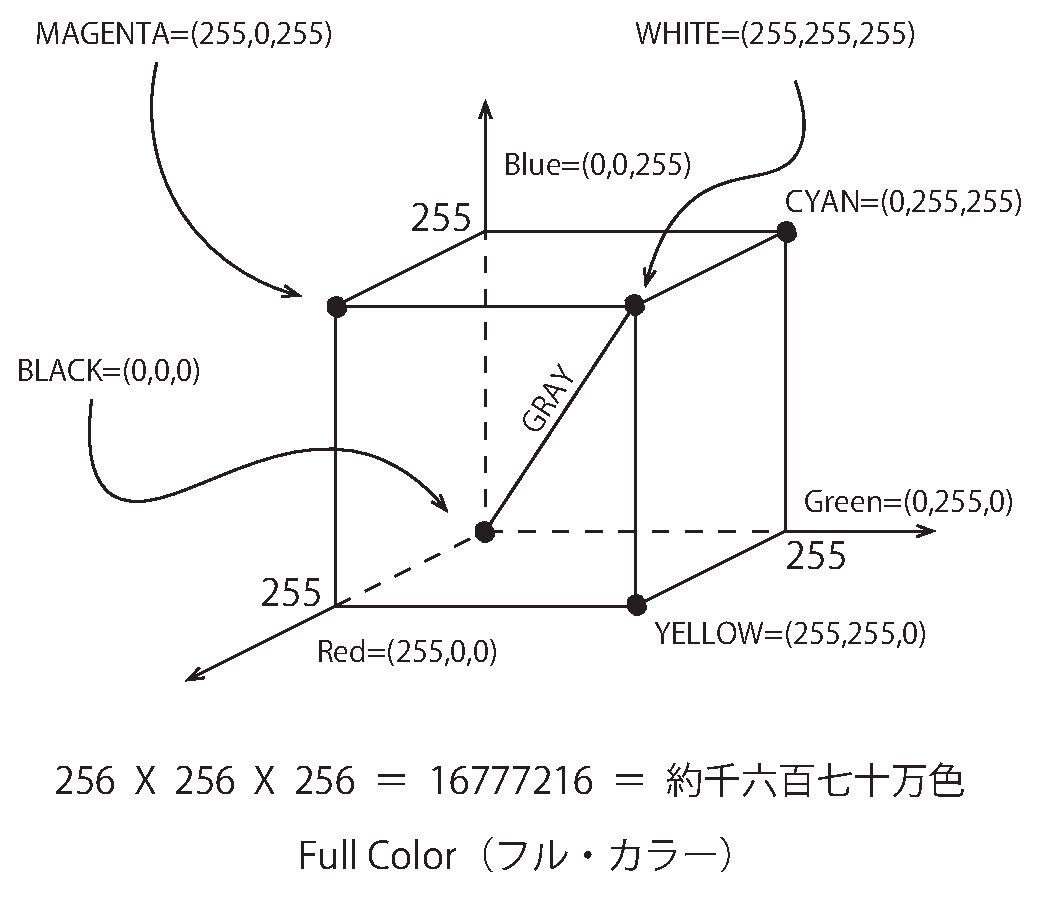
\includegraphics[width=0.5\hsize]{figures/eps/pg02.eps}
%\caption[短い説明]{長い説明}
\label{ラベル2}
\end{figure}

\vspace{4cm}

n = random.randint(0, 7)は、0$\le$n$\le$7 の範囲の整数をランダムに生成しています

確認のために、print(n) を一行入れてみたら理解の助けになるかもしれません\\

【演習】
\begin{enumerate}
\item[(1)] 白と黒の場合の(Red,Green,Blue)の値を、実際に設定して確認してみよう
\item[(2)] Red,Green,Blueに同じ値を指定すると、灰色の濃さが変わることを確認しよう
\item[(3)] 自分で好みの色を作ってscreenを塗りつぶしてみよう
\item[(4)] FPSの値を変えて実行してみよう
\item[(5)] FPSの値を大きくしすぎると、どんな問題を生じる可能性があるか考えてみよう
\end{enumerate}

\subsection{各種図形の描画}

\begin{center}
\includegraphics[width=0.5\hsize]{figures/eps/pg04-1.eps}
\end{center}

各種図形を描くときの、共通の引数としてsurfaceとcolorがあります

\begin{itemize}
\item surfaceは、その図形を描画する盤面(pygame.display.set\_modeで生成した)
\item 色の措定colorは、Red,Green,Blueのタプル
\end{itemize}

以下では、個々の図形のそのほかの引数について説明します

\begin{enumerate}

  \item[(1)] 円:pygame.draw.circle(Surface, color, position, radius, width=0)

  \begin{itemize}
  \item 円の中心位置positionは、X座標とY座標のタプル
  \item 円の半径radiusは整数値
  \end{itemize}

  \item[(2)] 線:pygame.draw.line(Surface, color, start\_position, end\_position, width=1)

  \begin{itemize}
  \item 始点start\_positionと終点end\_positionは、各々X座標とY座標のタプル
  \item 線の幅width=1はデフォルト引数(=1なら省略可能)
  \end{itemize}

  \item[(3)] 矩形:pygame.draw.rect(Surface, color, Rect, width=0)

  \begin{itemize}
  \item 線の幅width=0はデフォルト引数(=0なら省略可能)
  \item 矩形を納めるRectは、left, top, width, height のタプル
  \end{itemize}

  \item[(4)] 楕円:pygame.draw.ellipse(Surface, color, Rect, width=0)

  \begin{itemize}
  \item 楕円が収まるRectを、left, top, width, height のタプルで指定
  \end{itemize}

\end{enumerate}

\begin{center}
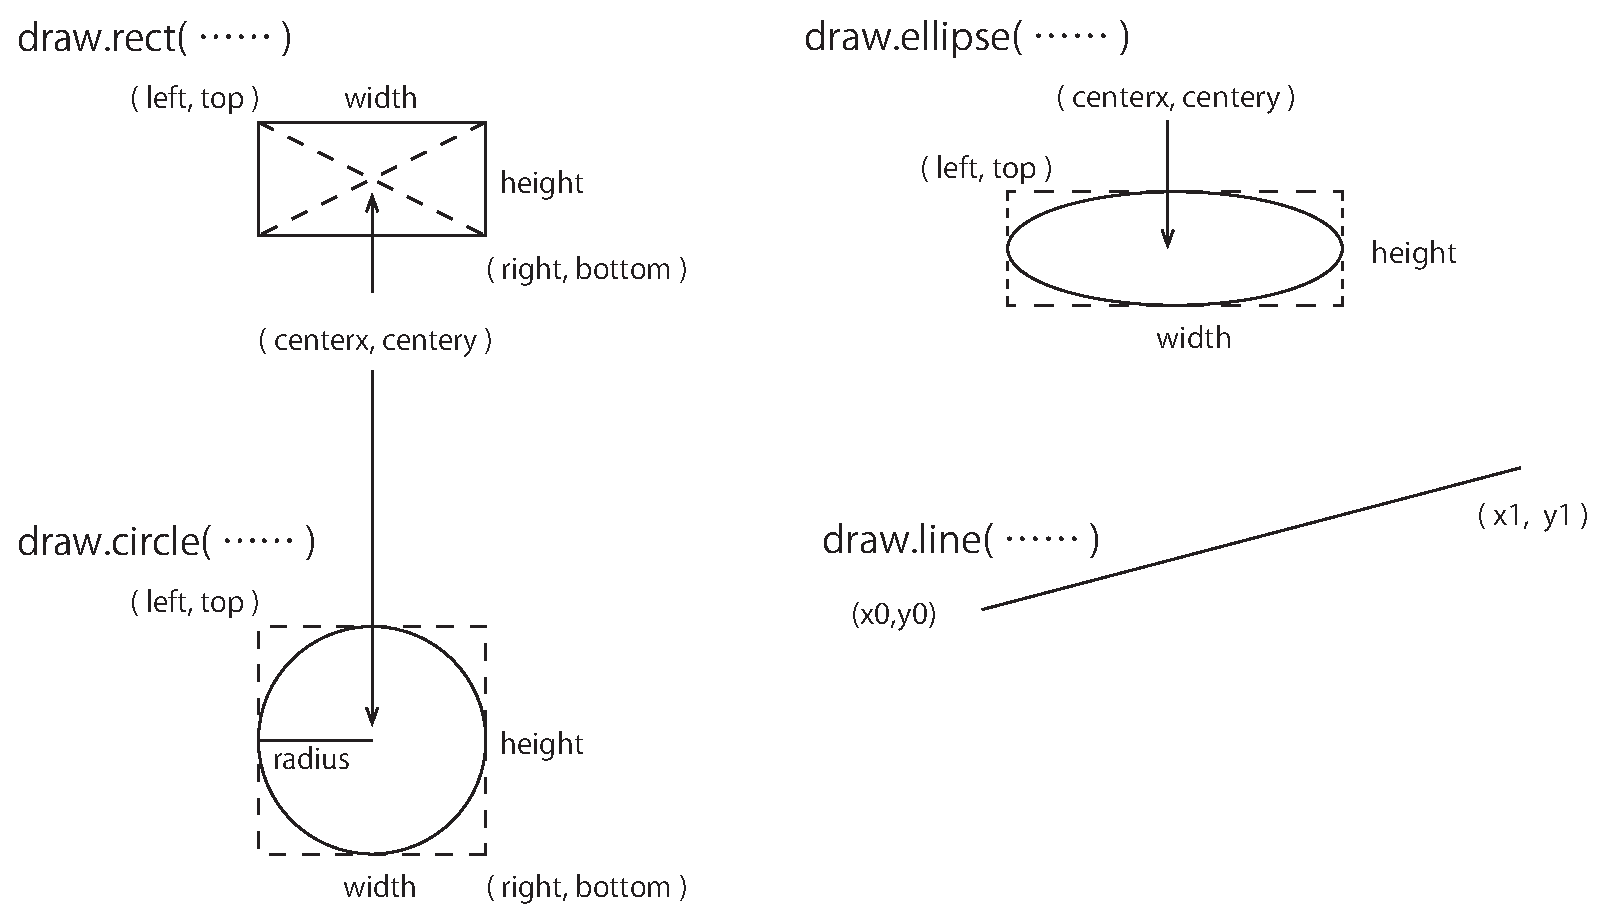
\includegraphics[width=0.6\hsize]{figures/eps/pg03.eps}
\end{center}

%\newpage

次の作図を試してみましょう
\begin{itemize}
\item surfaceの中央( WIDTH//2, HEIGHT//2)に、半径radius(=100ピクセル)の円Circle
\item surfaceの左上( left=0, top=0 )を始点、右下( right=WIDTH-1, bottom=HEIGHT-1 )を終点とする線Line
\end{itemize}

\begin{lstlisting}[caption=CircleとLine,label=]
import sys
import pygame
from pygame.locals import QUIT

pygame.init()
WIDTH = 640
HEIGHT = 480
WSIZE = (WIDTH, HEIGHT)
surface = pygame.display.set_mode( WSIZE )
pygame.display.set_caption( 'CircleとLine' )
clock = pygame.time.Clock()
FPS = 1

WHITE = (255,255,255)
r = 220
g = 120
b = 0
xc = WIDTH//2
yc = HEIGHT//2
radius = 100
left = top = 0
right = WIDTH - 1
bottom = HEIGHT -1

while True:
    for event in pygame.event.get():
        if event.type == QUIT:
            pygame.quit()
            sys.exit()
    surface.fill( WHITE )
    pygame.draw.circle( surface, (r, g, b), (xc, yc), radius, width=5 )
    pygame.draw.line( surface, (0, 0, 255), (left, top), (right, bottom) )
    pygame.display.update()
    clock.tick( FPS )
\end{lstlisting}

\begin{table}[htb]
\begin{center}
    \begin{tabular}{cc}
    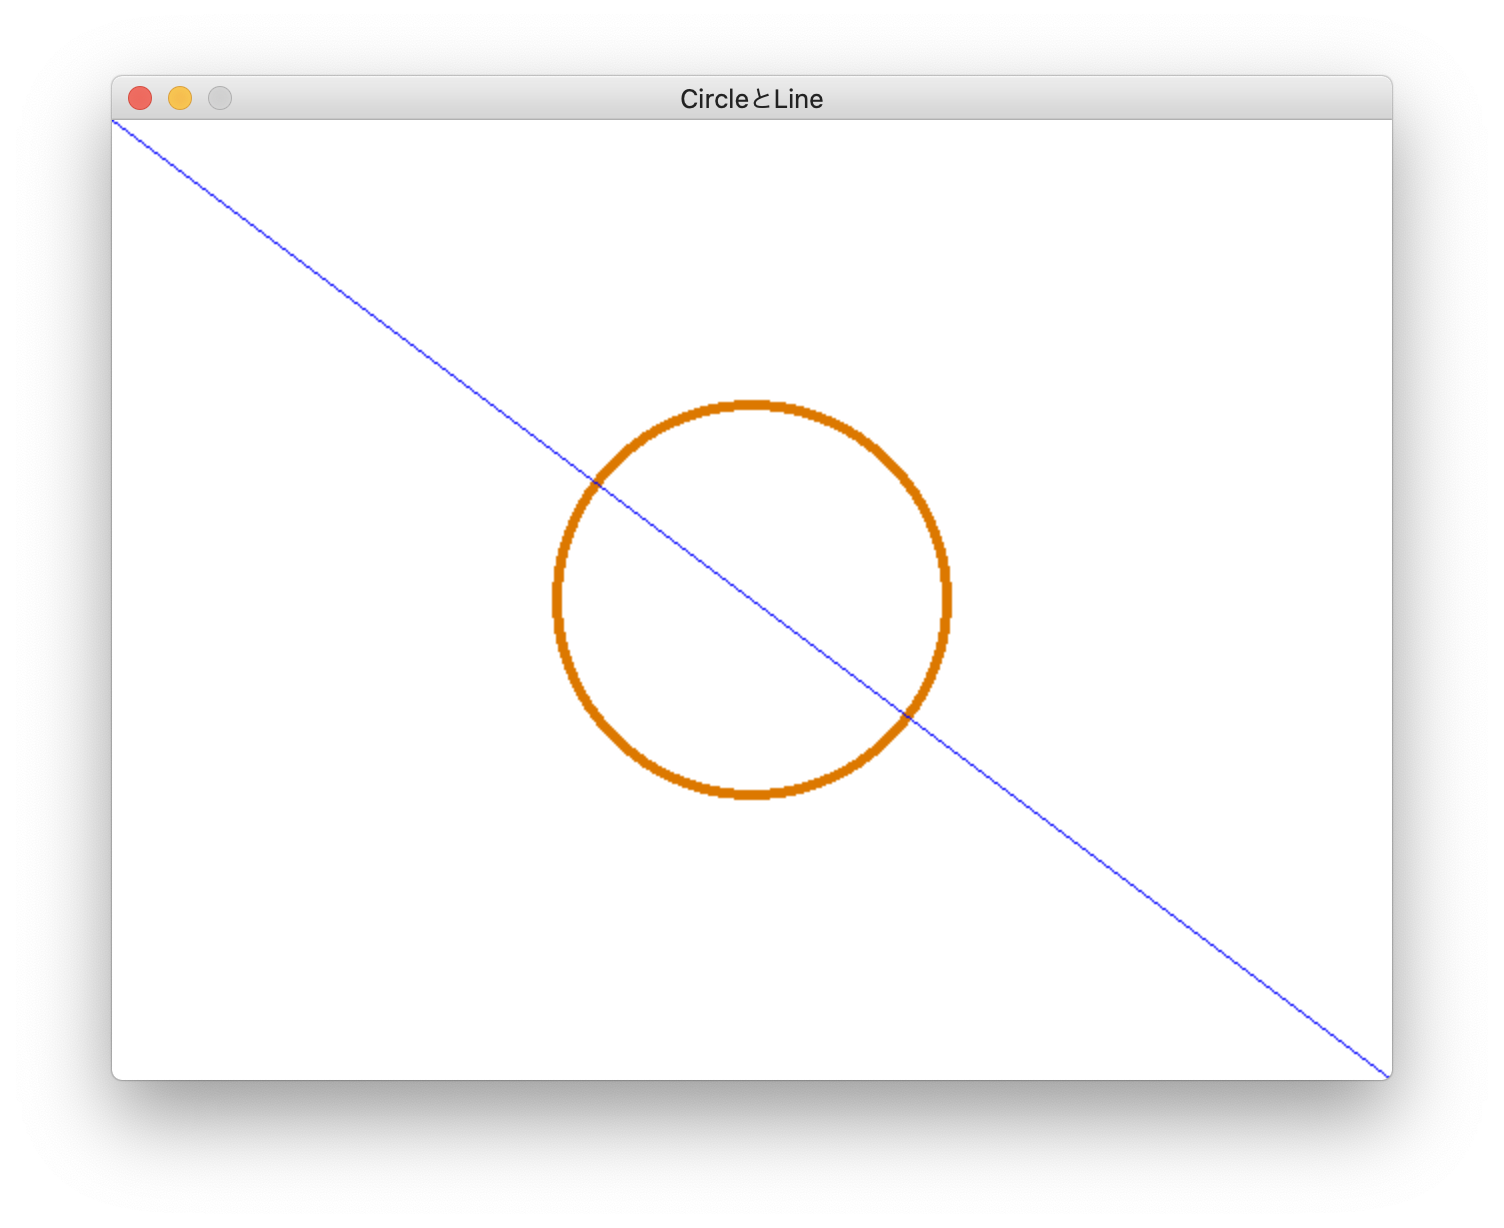
\includegraphics[width=0.45\hsize]{figures/eps/linecircle.eps} & 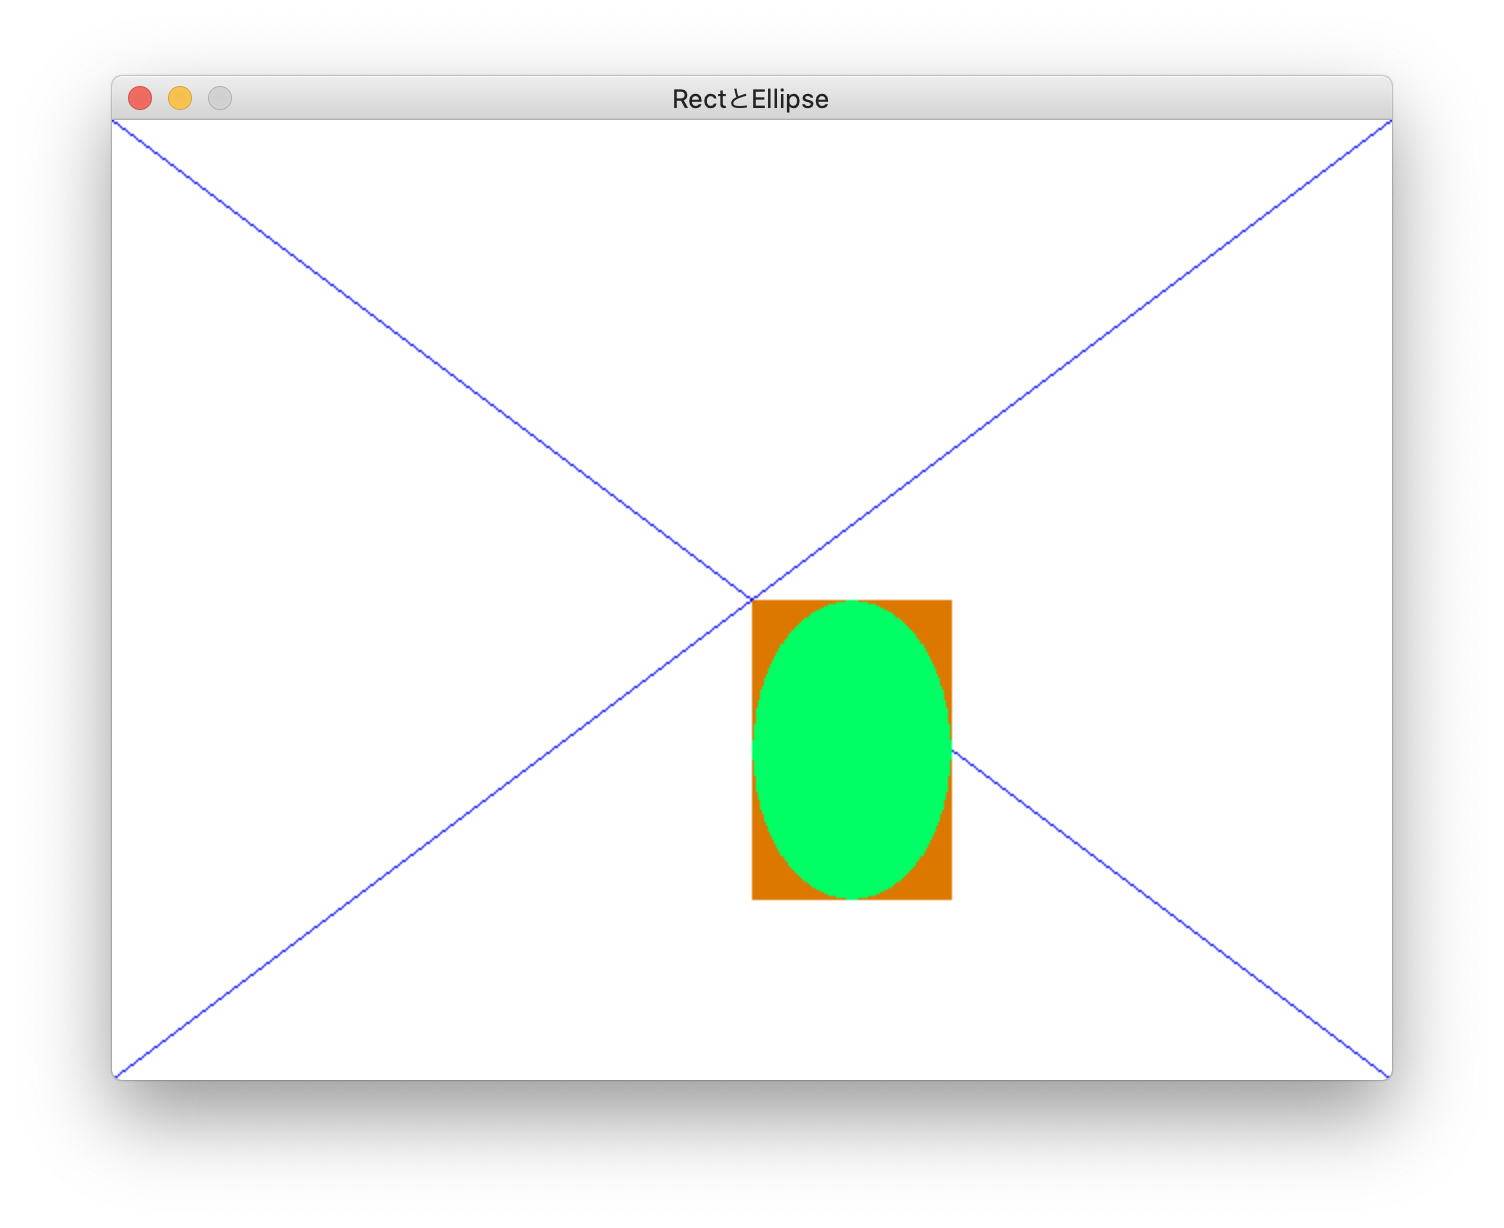
\includegraphics[width=0.45\hsize]{figures/eps/ellipserect.eps}
  \end{tabular}
\end{center}
\end{table}

次の作図を試してみましょう
\begin{itemize}
\item surfaceの中央( WIDTH//2, HEIGHT//2)を四角形Rectの左上の点(left, top)とし、幅widthを100、高さheightを150のRect
\item 上記のRectに収まる楕円Ellipse
\end{itemize}

\begin{lstlisting}[caption=RectとEllipse,label=]
import sys
import pygame
from pygame.locals import QUIT, Rect

pygame.init()
WIDTH = 640
HEIGHT = 480
WSIZE = (WIDTH, HEIGHT)
surface = pygame.display.set_mode( WSIZE )
pygame.display.set_caption( 'RectとEllipse' )
clock = pygame.time.Clock()
FPS = 1

WHITE = (255,255,255)
r = 220
g = 120
b = 0
xc = WIDTH//2
yc = HEIGHT//2
width = 100
height = 150
rect = Rect(xc, yc, width, height)

while True:
    for event in pygame.event.get():
        if event.type == QUIT:
            pygame.quit()
            sys.exit()
    surface.fill( WHITE )
    pygame.draw.line( surface, (0, 0, 255), (0, 0), (639, 479) )
    pygame.draw.line( surface, (0, 0, 255), (639, 0), (0, 479) )
    pygame.draw.rect( surface, (r, g, b), (xc, yc, width, height) )
    pygame.draw.ellipse( surface, (0, 255, 100), rect )
    pygame.display.update()
    clock.tick( FPS )
\end{lstlisting}

【演習】randomをimportして、次のことを試してみましょう
( from random import randint )
\begin{enumerate}
\item[(1)] circleの中心のx座標をrandint(0, WIDTH-1)で、y座標も同様にして作図してみよう
\item[(2)] circleの半径を、乱数randint(1,60)程度で発生させ、中心座標と共に変化させてみよう
\item[(3)] 乱数でr=randint(0,255)、g、bを作り、タプル(r,g,b)でcircleの色を指定してみまよう
\item[(4)] ellipseやrectあるいはlineなどを、乱数を使ってsurface上に表示させてみよう
\item[(5)] surface.fill()をコメントアウトしてみよう
\end{enumerate}%

\begin{center}
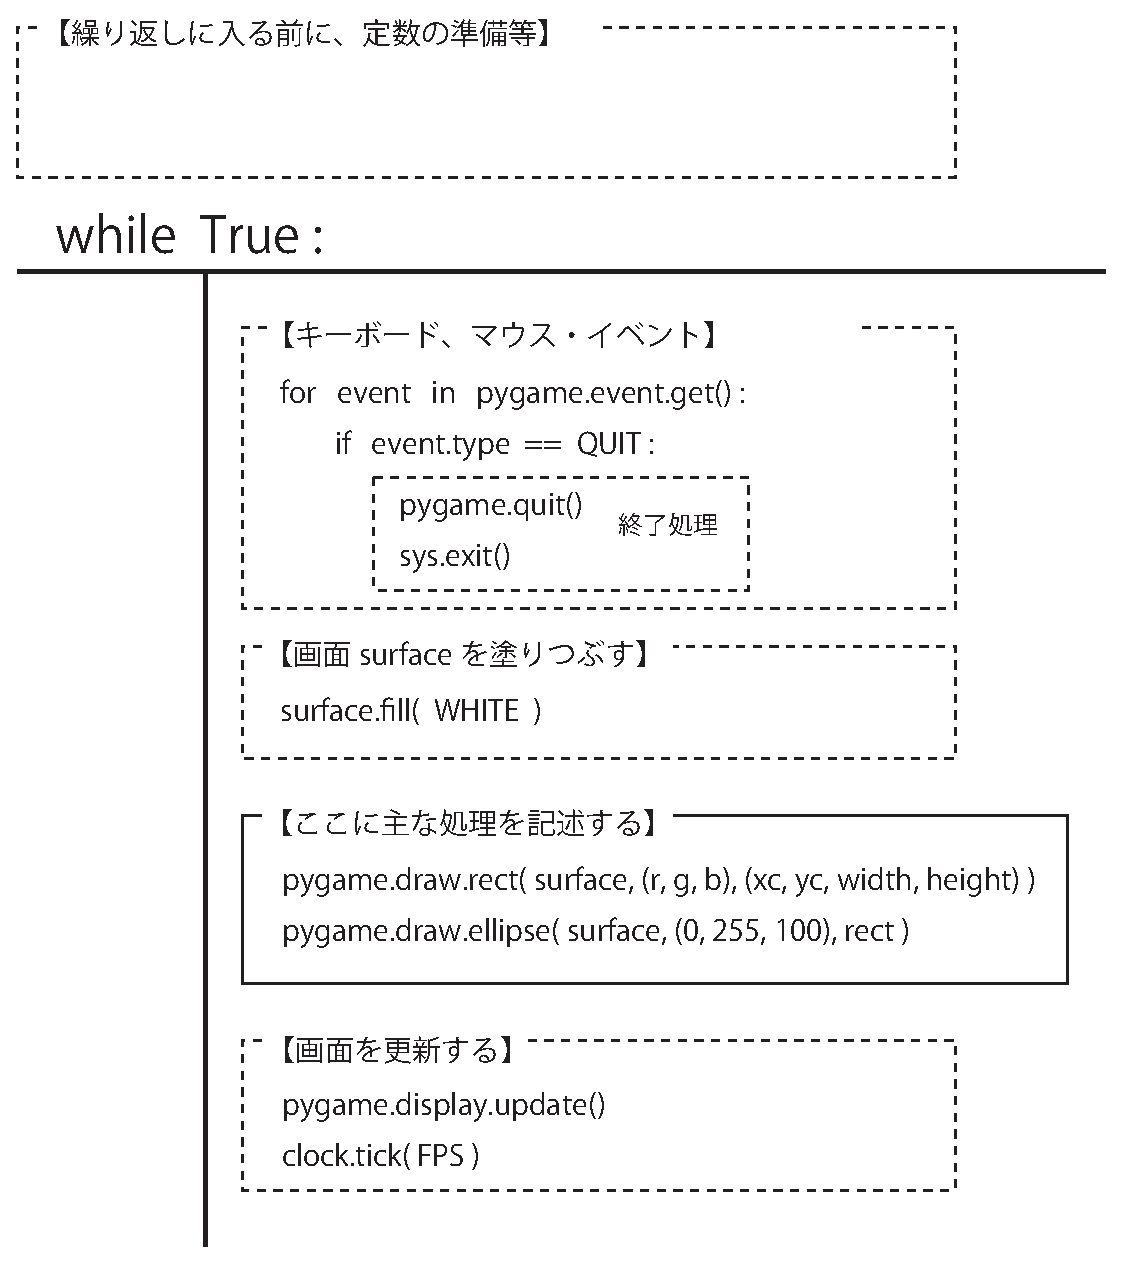
\includegraphics[width=0.6\hsize]{figures/eps/zushi.eps}
\end{center}

\subsection{図形の移動}

circleで描いたボールの y 座標を、フレーム更新のたびに増加させて、ボールを動かします

ボールの y 座標が、surfaceのHEIGHTに達したら終わります

QUITをイベントとして検出した際に実行される終了処理を、fine()関数にまとめています

surface.get\_rect().width によって得られるのは、WIDTH

surface.get\_rect().height によって得られるのは、HEIGHT

\lstinputlisting[caption=図形の移動,label=pg05]{programs/python/pg05.py}

\begin{center}
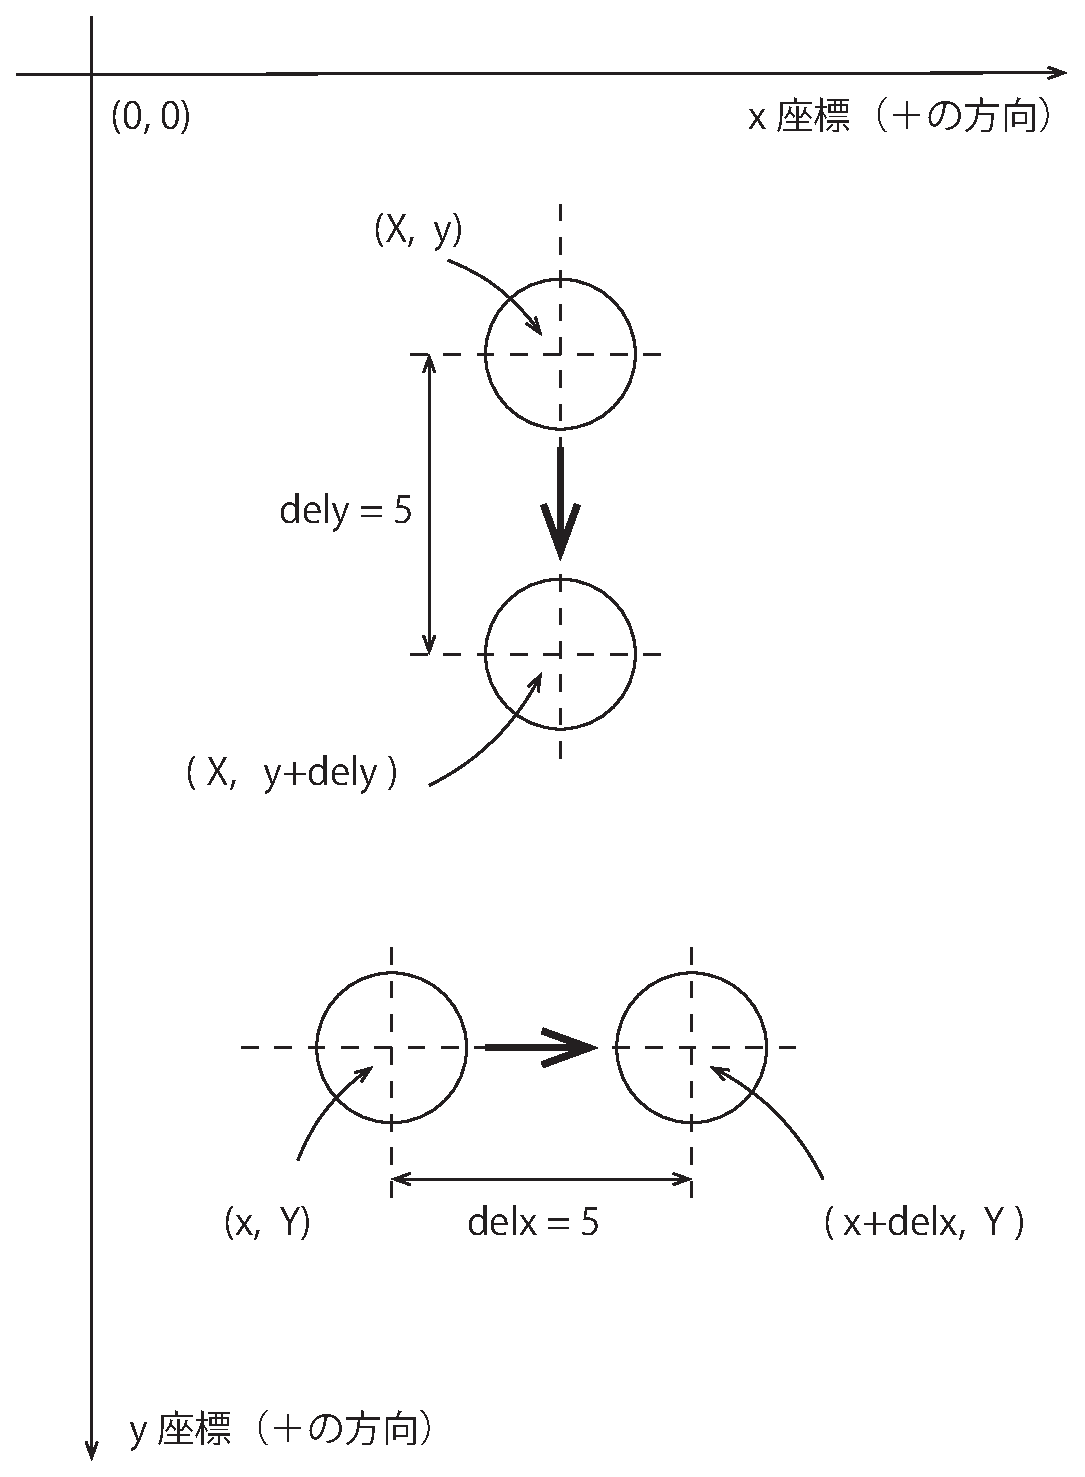
\includegraphics[width=0.4\hsize]{figures/eps/pg05.eps}
\end{center}

【演習】
\begin{enumerate}
\item[(1)] FPSを変えずにボールの移動するスピードを変えるには、どうすればいいでしょう
\item[(2)] ボールが、画面中央を下から上に動くようにプログラムを書き直してみましょう
\item[(3)] ボールが、画面中央を左から右に動くようにプログラムを書き直してみましょう
\item[(4)] ボールが、画面中央を右から左に動くようにプログラムを書き直してみましょう
\item[(5)] ボールが、画面の左上から右下に向かって動くようにプログラムを書き直してみましょう
\item[(6)] ボールが、画面の左下から右上に向かって動くようにプログラムを書き直してみましょう
\item[(7)] x方向座標値の増分とy方向座標値の増分の値が等しくない様にしたら、ボールの動きはどうなりますか
\end{enumerate}

\subsection{壁で反射するボール}

\begin{center}
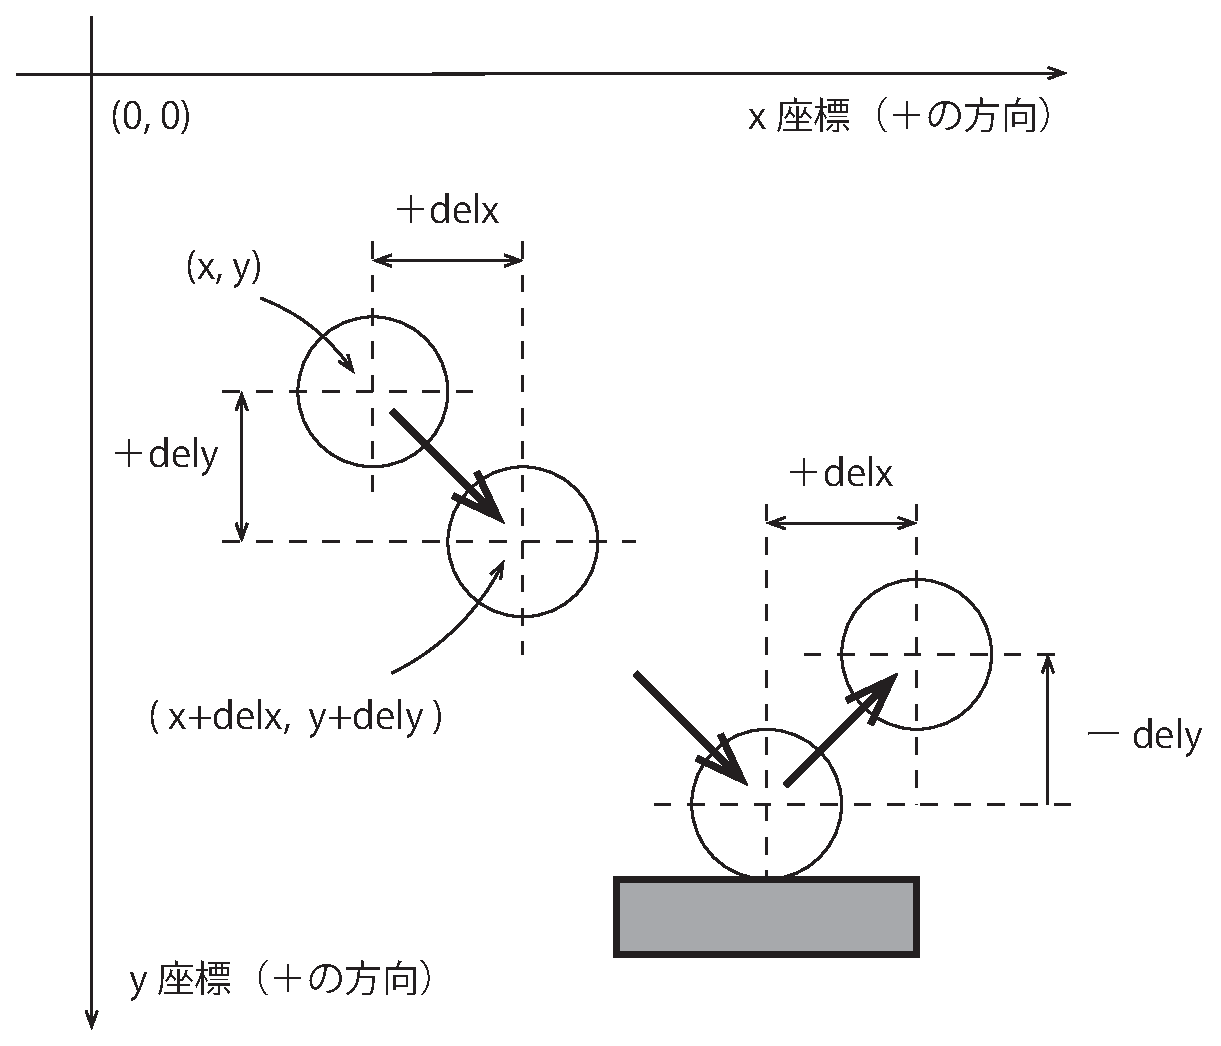
\includegraphics[width=0.5\hsize]{figures/eps/pg06.eps}
\end{center}

circleで描いたボールの y 座標を、フレーム更新のたびに増加させて、ボールを動かします

ボールの y 座標が、surfaceのHEIGHTに達したら、y 方向の移動量をマイナスの値にしています

ボールの y 座標が、surfaceの上端に達したら、y 方向の移動量をプラスの値に戻しています

\lstinputlisting[caption=反射:位置変化量の符号を反転,label=pg06]{programs/python/pg06.py}

ボールが上下 y 方向で反射するように、y 方向の移動量の符号を反転しているのは前の例と同じです

ボールを左右 x 方向でも反射するように、x 方向の移動量の符号も反転させています

最初にボールを放出する位置 x 座標を、乱数で決めています

\lstinputlisting[caption=反射,label=pg07]{programs/python/pg07.py}

\subsection{ラケットの導入}

%\begin{figure}[h]
%\vspace*{-0.85cm}
\begin{center}
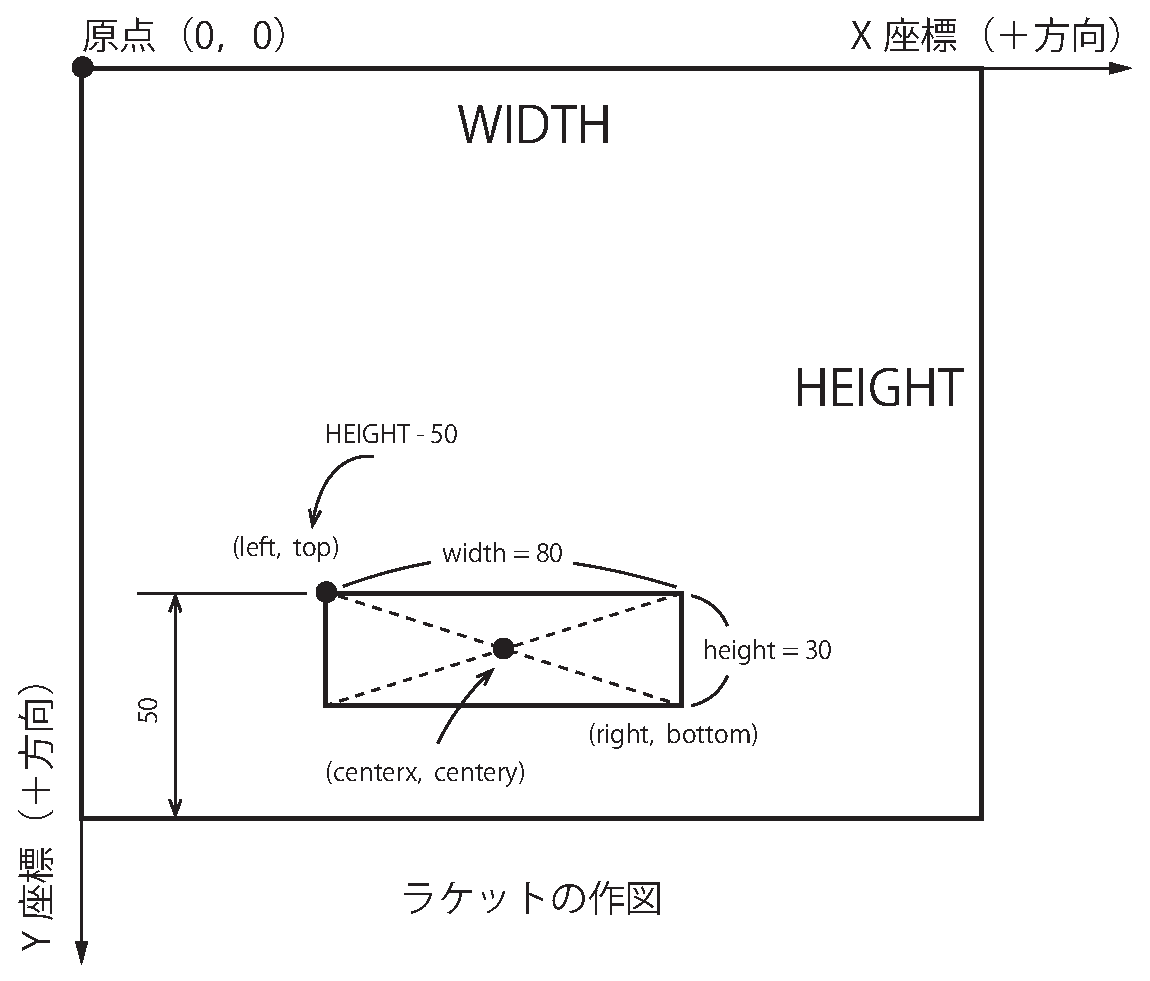
\includegraphics[width=0.5\hsize]{figures/eps/pg11.eps}
\end{center}
%\end{figure}

ラケットをpygameのRect(クラスのオブジェクト)として作図し、
それを左右の矢印キーを使って動かせるようにします

Rectクラスのオブジェクトは、次の3つの方法のどれかを使って生成できます

\begin{itemize}
\item pygame.Rect( left, top, width, height )
\item pygame.Rect( (left, top), (width, height) )
\item pygame.Rect( Rectオブジェクト )
\end{itemize}

Rectクラスは次のようなプロパティを持っており、値を設定することができます

top, left, bottom, right,
topleft, bottomleft, topright, bottomright,

midtop, midleft, midbottom, midright,
center, centerx, centery, size, width. height, w, h

このプログラム例では、ラケットの初期位置をラケットのRectの左肩(left,top)について、
画面の中央の縦線をleftに、画面の下端から50ピクセル上をtopに、重ねています

また、キーボードからのイヴェントを拾うkey\_event()関数を新たに定義して、
ゲームのメインループの記述を単純にしました

\begin{lstlisting}[caption=ラケットのRectを描画,label=pg08-0]
import sys
import pygame
from pygame.locals import QUIT, Rect
import random

def fine():
    pygame.quit()
    sys.exit()

def key_event():
    for event in pygame.event.get():
        if event.type == QUIT:
            fine()

pygame.init()
WIDTH = 640
HEIGHT = 480
WSIZE = (WIDTH, HEIGHT)
surface = pygame.display.set_mode( WSIZE )
pygame.display.set_caption( 'Squash(Bounding Ball)' )
clock = pygame.time.Clock()
FPS = 20

WHITE = (255,255,255)
# ボールのdraw.circleのために
RED = (255,0,0)
RADIUS = 10
x = random.randint( 0, WIDTH-1 )
y = 0
delx = dely = 5
# ラケットのdraw.rectのために
GREEN = (0,255,0)
SIZE = (WIDTH//2, HEIGHT-50, 80, 10)
racket = Rect( SIZE )

while True:
    key_event()
    surface.fill( WHITE )
    pygame.draw.rect( surface, GREEN, racket )
    pygame.draw.circle( surface, RED, (x,y), RADIUS )
    # 上下の壁でボールの反射
    if y>=HEIGHT or y<0:
        dely = -dely
    # 上下の壁でボールの反射
    if x>=WIDTH or x<0:
        delx = -delx
    # ボールの中心座標を更新
    x += delx
    y += dely
    pygame.display.update()
    clock.tick( FPS )
\end{lstlisting}%

sizeやwidth及びheightの属性の変更は、四角形の大きさを変更することになり、
それ以外のプロパティの変更は、四角形の大きさを変えずに、描画位置を変更することになります

このプログラム例では、ラケットの Rect の centerx プロパティを操作しています

キーボードの左右の矢印キーのイベントを拾って、
右矢印(K\_RIGHT)の時は racket.centerx+=15、左矢印(K\_LEFT)の時は racket.centerx-=15 のように変えることによって、
描画位置を変えています

\lstinputlisting[caption=ラケット,label=pg08]{programs/python/pg08.py}

\subsection{ラケットとボールの干渉}

ボールの位置はwhile True:のループの中でその都度動いていますから、
毎回ボールのRectを定義し直しては、
ラケットのRect と ボールのRect との間に重なりが生じたか否かを、colliderect()メソッドを使って検出しています

左右方向の矢印キーを押した時、ラケットの動きをスクリーンの幅の中に制限
(ラケットのRectの右側が画面のWIDTH未満であることや、ラケットのRectの左側が画面の左端=0より大きい範囲に制限)
する様にしています

%キーボード・マウスのイベントをチェックしている部分を、関数key\_event()にまとめています

\lstinputlisting[caption=ラケットとボールの干渉検出,label=pg09]{programs/python/pg09.py}

ボールを打ち返し損じた場合、Game Overとprintして終了(whileのループをbreakで抜けてfine()処理に入る)
するようにしています

\subsection{文字テキストの表示}

「Game Over !」の文字テキストを、ゲームっぽく大きな文字で画面の中央に表示させます

textというオブジェクトでは、文字テキストのフォントサイズ、色、表示場所を指定しています

文字の表示位置も、Rectによって幾何情報を保持している点に注目しましょう

font.render()(これはfontオブジェクトのrenderメソッド)は、指定文字を描画したSurfaceを返しますので、
その文字を描画したSurfaceを、下地のSurfaceの上に重ねて描画する必要があります

surface.blit()(これはsurfaceオブジェクトのblitメソッド)は、画像を他の画像の上に重ねて描画するメソッドです

\lstinputlisting[caption=文字テキストの表示など,label=pg10]{programs/python/pg10.py}

ボールを打ち返し損じた場合、whileのループをbreakで抜けてfine()処理に入ることで
プログラムを終了するようにしているので、せっかくのメッセージを見ることができません
(breakをコメントアウトして、終了の検出はマウスでWindowを閉じるイベントを発生させる
ことに頼るようにしたらよいかもしれません)

ボールを放出する位置のほか、
ボールを放出する方向(左右)も乱数を使って決めています
(具体的には、ボール移動の x 方向の移動量の符号を乱数で決めています)

ラケットでボールをはね返したら10ポイントを加算することとし、
キャプションにその時点での得点を表示するようにしています

\begin{center}
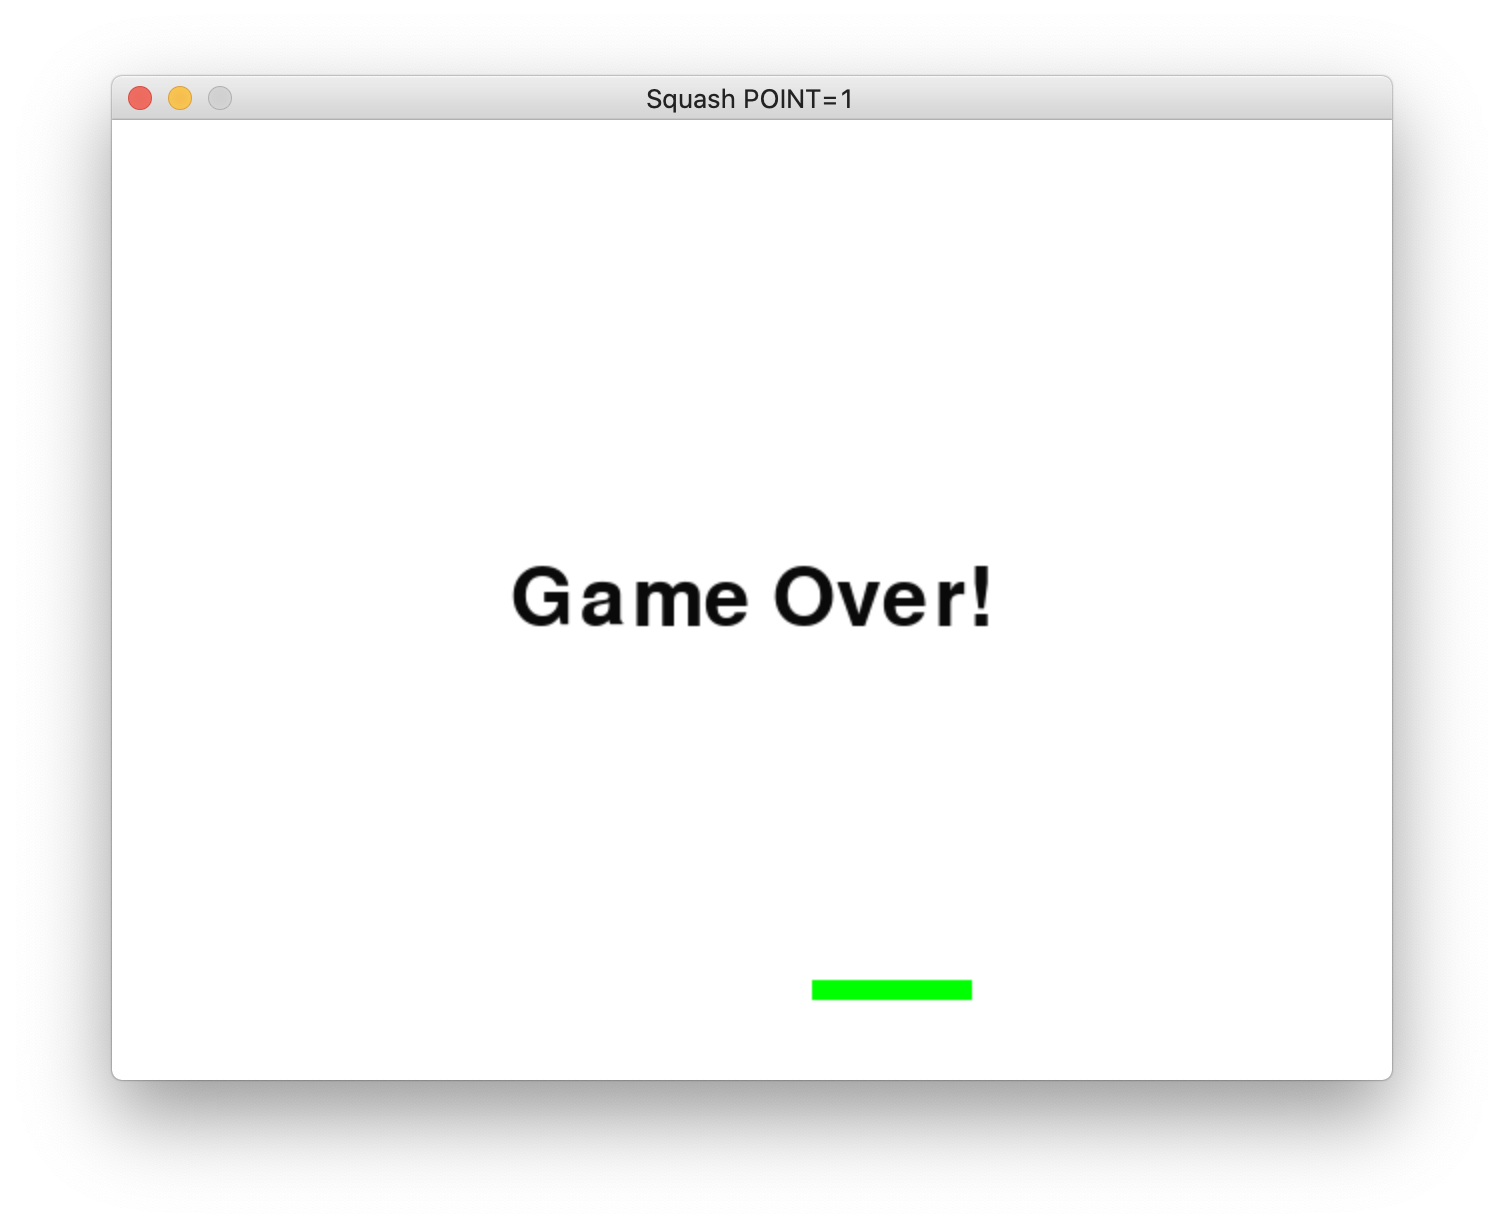
\includegraphics[width=0.4\hsize]{figures/eps/pg10.eps}
\end{center}

【演習】
\begin{enumerate}
  \item[(1)] 乱数を使って、角度30度〜150度(=180度ー30度)の範囲でボールが放出されるように直してみましょう
  \item[(2)] 青いボールを追加して放出し、2つのボールをラケットで打ち返すゲームに直してみましょう
\end{enumerate}

\newpage

\section{オブジェクト指向}

ここまでに作成してきたプログラムを、オブジェクト指向の考え方を使って書き換えていきます\\

まず、このゲームを構成しているもの(オブジェクト:Object)を列挙して、
それらのもの(オブジェクトあるいはインスタンスとも呼ばれる)が具体的にどのような特性(プロパティー:Property)を持っているのかを考えてみます

とりあえず思いつくものをあげてみると、次の4つでしょうか

\begin{itemize}
  \item ボール:色、形(円)、大きさ(半径)、位置(x,y座標)、スピードなど
  \item ラケット:色、位置(x,y座標)など
  \item 表示するメッセージ:文字列("Game Over!")、色、フォント、サイズ、表示位置(x,y座標)など
  \item スカッシュを行う空間(ボールが飛び交う場):背景色、大きさ(幅、高さ)、キャプションなど
\end{itemize}

基本的に、それぞれのオブジェクトは自分自身の特性(プロパティ)を知って(保持して)いますし、
自分自身のプロパティを操作するメソッド(関数)を持っています。
一方、自分以外のオブジェクトのことは分かりません。つまり他のオブジェクトの情報は持たないようにして、
それぞれのオブジェクトが、できるだけ独立して存在させるようにすると見通しがよくなります。
%(詳しくは「Gofによるデザインパターン」などについて勉強すると良いでしょう)

しかし実際のゲームを考えると、ボールのオブジェクトとラケットのオブジェクトの間の干渉や、
スカッシュ競技場の壁にボールが当たったかどうか、
またボールが後ろ(下)の壁を通り越してしまい、ゲーム終了になったかどうか
など、これらオブジェクトとオブジェクトの間の相互の関わりを調べて操作する必要が生じてきます。

そこで、ゲームの進行を司るものとしてGameというオブジェクトを、
上の4つのオブジェクトに追加して、このゲームを構成することにしましょう

オブジェクトの設計図のことをクラス(Class)といいます

ここから、上で述べた5つのオブジェクトそれぞれについて、クラスの設計を進めていきます

なお、この後クラスから生成される具体的なものを、オブジェクトではなく、インスタンスと呼ぶことがあります

\subsection{main.pyの処理}

if \_\_name\_\_ == '\_\_main\_\_':とかくと、この下の行からプログラムの実行を開始することになります

ここでは、
Gameクラスのオブジェクトであるgameを生成し、その後
gameオブジェクトの中のstart()というメソッドを実行するように指示しています

\begin{lstlisting}[caption=main.py,label=prog01-1]
if __name__ == '__main__':
    game = Game()
    game.start()
\end{lstlisting}%

実際にGameクラスを記述していく際には、
start()メソッドが呼び出されるのですから、Gameクラスの中にstart()メソッドを用意しなければなりません

仮にstart()メソッドでprint()関数だけを実行させることにしますと

\begin{lstlisting}[caption=main.pyとGame.py,label=prog01-2]
class Game:
    def start(self):
        print('Gameクラスのstart()メソッド')

if __name__ == '__main__':
    game = Game()
    game.start()
\end{lstlisting}%

クラスの中に、def \_\_init\_\_(self):として、予め決まった名前のメソッドを定義することができます

このメソッドはコンストラクタと呼ばれ、クラスのオブジェクトが生成される際、最初に一度だけ実行されます

start()メソッドの実行文を\#でコメントアウトしてしまい、gameオブジェクトの生成だけ行ってみると、コンストラクタだけが実行されることが分かります

また、start()メソッドのコメントを外してみると、コンストラクタ実行後にstart()メソッドが実行されることを確認できます

\begin{lstlisting}[caption=main.pyとGame.py,label=prog01-3]
class Game:
    def __init__(self):
        print('Gameクラスのコンストラクタ')

    def start(self):
        print('Gameクラスのstart()メソッド')

if __name__ == '__main__':
    game = Game()
    # game.start()
\end{lstlisting}%

さて、ゲームのプログラム作りに話を戻します

mainプログラムを、まずは次の通り書くことにします

\begin{lstlisting}[caption=main.py,label=p0]
from Game import Game

if __name__ == '__main__':
    game = Game()
    game.start()
\end{lstlisting}

\subsection{画面のクラス:Screen}

Screenクラスでは、スカッシュを行う場所、ボールの飛び交う場を定義します

このクラスが持つ主な特性値(プロパティ)は次の通りです

\begin{itemize}
  \item 画面の幅(WIDTH)
  \item 画面の高さ(HEIGHT)
  \item 描画面(surface)
\end{itemize}

これらの特性値はコンストラクタ(\_\_init\_\_()メソッド)の中で、それぞれの初期値を設定しています

コンストラクタの引数には、デフォルトの値を設定しています

これらの特性値を操作するメソッドは2つです

\begin{itemize}
  \item fillメソッドは、\\fillメソッドによって、引数で受け取ったcolor色でsurfaceを塗りつぶします
  \item captionメソッドは、\\set\_captionメソッドによって、引数で受け取った文字列をWindowのタイトルバーに表示します
\end{itemize}

\begin{lstlisting}[caption=Class Screen,label=p2]
import pygame

class Screen:
    def __init__(self, width=600, height=600):
        self.WIDTH = width
        self.HEIGHT = height
        SIZE = (width, height)
        self.surface = pygame.display.set_mode( SIZE )

    def fill(self, color=(255, 255, 255)):
        self.surface.fill( color )

    def caption(self, str):
        pygame.display.set_caption( str )
\end{lstlisting}

\subsection{ゲームの進行を司るクラス:Game}

ゲームの進行を司るクラスGameは、
今の段階では、そのコンストラクタの中でScreenクラスのオブジェクトをscreenという名前で生成し、それを表示しています

Gameクラスのkey\_event()メソッドでは、Windowを閉じる時のイベントQUITを取得すると、終了処理fine()メソッドを呼び出しています

start()メソッドは、このゲームの主な処理(繰り返し)を行うメソッドなので、この中に具体的なゲームの進行を記述していきます

この後、このGameクラスを少しずつ改造していきます

\begin{lstlisting}[caption=Gameクラス(screenオブジェクトを生成),label=p1]
import sys
import pygame
from pygame.locals import QUIT
from Screen import Screen

class Game():
    WHITE = (255, 255, 255)
    def __init__(self):
        pygame.init()
        self.WIDTH = 640
        self.HEIGHT = 480
        self.screen = Screen( self.WIDTH, self.HEIGHT )
        self.screen.caption( "Squash game" )
        self.clock = pygame.time.Clock()
        self.FPS = 30

    def fine(self):
        pygame.quit()
        sys.exit()

    def key_event(self):
        for event in pygame.event.get():
            if event.type == QUIT:
                self.fine()

    def start(self):
        game_over = False
        while not game_over:
            self.key_event()
            self.screen.fill( Game.WHITE )
            # ↓ ここからゲームの進行を記述していく

            # ↑ ゲーム進行の記述はここまで
            pygame.display.update()
            self.clock.tick(self.FPS)
\end{lstlisting}

クラスの中で定義する関数(メソッドと呼ばれる)の第1引数には、必ず「self」と指定します

selfは、そのクラスから生成される「オブジェクトそれ自身」のことを指しています

「self.変数名」と書いたとき、その変数はオブジェクト変数と呼ばれ、selfすなわち、
クラスから生成された具体的なオブジェクトの中に保持されている変数という意味になります。
そのクラスから複数のオブジェクトが生成された場合には、それぞれのオブジェクトが個別に持っている変数を指していることになります

一方、「self.」を付けていない変数等は、その関数内でだけ通用するローカルな変数になりますので、
当該オブジェクトの中の他のメソッドから参照することはできませんし、またそのクラスの外から参照することもできません

なお、メソッドを呼び出すときは、selfを除いた形で引数を記述します

この他に、「クラス名.変数名」と記述するクラス変数というものがあります。
クラスから生成されるオブジェクトの、いずれにも共通に保持されている変数になります

ここの例では、WHITEというタプルの値をクラス変数として定義し、
fill()メソッドへの引数に Game.WHITE という名前で指定しています

\subsection{ボールのクラス:Ball}

Ballのクラスが持つ特性値(プロパティ)として次のものを考えます

\begin{itemize}
  \item ボールの色(COLOR)
  \item ボールの形(円は楕円ellipseの一種)
  \item ボールの大きさ(円の半径RADIUS)
  \item ボールの現在位置(Rectの特性値、left,top,width,height,およびcenterx,centeryで)
  \item ボールの進む速さ(SPEED)
  \item ボールの進んでいる方向(dirx, diry)
  \item ボールが飛び回る場所(surface)
\end{itemize}

これらのプロパティは、コンストラクタ(\_\_init\_\_()メソッド)の中で、それぞれの初期値を設定しています

コンストラクタの引数には、デフォルトの値を引数として設定していますので、
特別な変更を要しない限り、オブジェクト生成の際にその引数として値を明示的に書く必要がありません

また、Ballクラスは、Rectクラスを継承しているので、
Rectクラスが持っているプロパティ(left、top、centerxなど)は、
そのままBallクラスにある他のプロパティと同じように扱うことができます\\

これらのプロパティを操作するメソッドとして次の5つを用意しました

\begin{itemize}
  \item drawメソッドは、\\ellipse関数を使って、surface上にRectの特性値が保持している現在位置に、指定の色COLORで、円を描画します
  \item stop\_ballメソッドは、\\ボールのSPEEDをゼロにして、ゲーム終了時に呼び出されることを想定しています
  \item movexメソッドは、\\指定のSPEED分だけ、現在ボールが進んでいる方向dirxに、Rectの特性値、即ち現在位置を移動させます
  \item moveyメソッドは、\\指定のSPEED分だけ、現在ボールが進んでいる方向diryに、Rectの特性値、即ち現在位置を移動させます
  \item movexyメソッドは、\\movex関数とmovey関数を順に呼び出して、Rectの特性値、即ちボールの現在位置を移動させます
\end{itemize}

最初に放出されるボールの進行方向を、コンストラクタの中で角度30度〜150度の間の乱数で作り出しています

movex()メソッドやmovey()メソッドでは、ボールの進行方向の角度を、度の単位で持っていることから、
それをラジアン単位に変換した上で、sin()関数やcos()関数を使ってボールの中心座標を計算しています

\begin{center}
  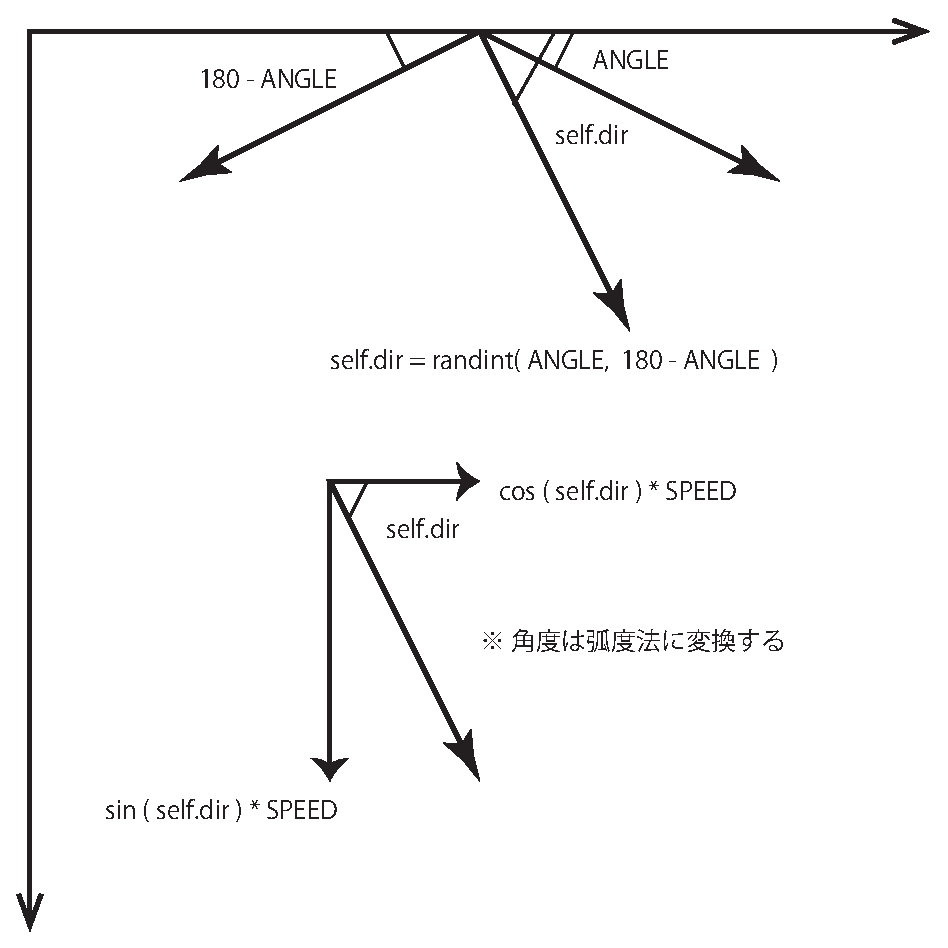
\includegraphics[width=0.4\hsize]{figures/eps/startball.eps}
\end{center}

\begin{lstlisting}[caption=Ballクラス,label=p3]
from math import sin, cos, radians
from random import randint
import pygame
from pygame.locals import Rect

class Ball( Rect ):
    def __init__(self, surface, color=(180, 180, 180),\
                        diameter=20, speed=10, start=(300,300)):
        self.surface = surface
        self.COLOR = color
        self.SPEED = speed
        ANGLE = 30
        self.dir = randint(ANGLE, 180 - ANGLE)
        self.left = start[0]
        self.top = start[1]
        self.width = diameter
        self.height = diameter

    def stop_ball(self):
        self.SPEED = 0

    def movex(self):
        self.centerx += int( cos(radians(self.dir)) * self.SPEED )

    def movey(self):
        self.centery += int( sin(radians(self.dir)) * self.SPEED )

    def movexy(self):
        self.movex()
        self.movey()

    def draw(self):
        pygame.draw.ellipse(self.surface, self.COLOR, self)
\end{lstlisting}

\begin{center}
  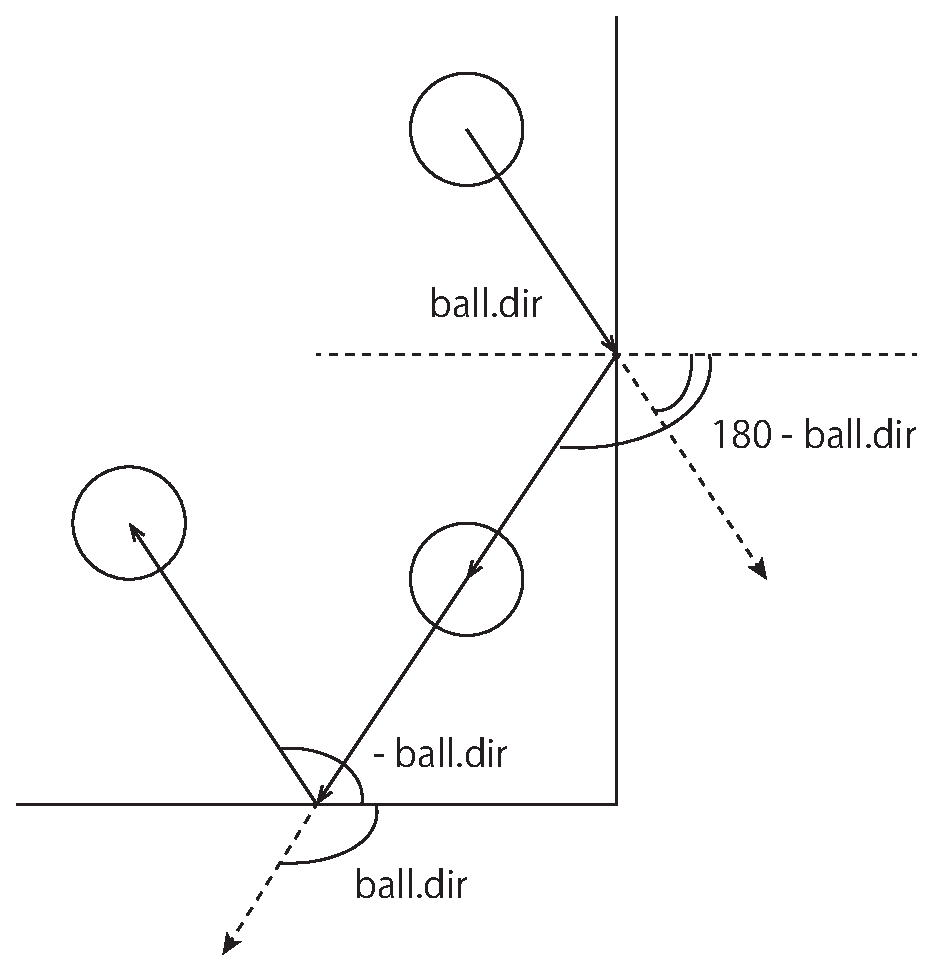
\includegraphics[width=0.4\hsize]{figures/eps/boundball.eps}
\end{center}

\subsubsection{Gameクラスの書き換え}

Ballクラスのオブジェクト赤いballを、Gameクラスのコンストラクタで生成し、
start()メソッドの中でそのballオブジェクトを描画ball.draw()したり、
ballオブジェクトの現在位置を動かしball.movexy()たりしています

また、Gameクラスのboundary()メソッドでは、
ballオブジェクトがscreenオブジェクトの横幅を超えて移動しようとしたとき、
また、ballオブジェクトがscreenオブジェクトの縦の長さを超えて移動しようとしたときに、
ballオブジェクトの進行方向を反転させています

\begin{lstlisting}[caption=Gameクラス(ballオブジェクトを追加),label=p1]
import sys
import pygame
from pygame.locals import QUIT
from Ball import Ball
from Screen import Screen

class Game():
    WHITE = (255, 255, 255)
    def __init__(self):
        pygame.init()
        self.WIDTH = 640
        self.HEIGHT = 480
        self.screen = Screen( self.WIDTH, self.HEIGHT)
        self.screen.caption("Squash game")
        self.clock = pygame.time.Clock()
        self.FPS = 30
        RED = (255,0,0)
        self.ball = Ball(self.screen.surface, color=RED)

    def fine(self):
        pygame.quit()
        sys.exit()

    def key_event(self):
        for event in pygame.event.get():
            if event.type == QUIT:
                self.fine()

    def boundary(self, ball):
        if not (0 < ball.centerx < self.WIDTH):
            ball.dir = 180 - ball.dir
        if not (0 < ball.centery < self.HEIGHT):
            ball.dir = -ball.dir

    def start(self):
        game_over = False
        while not game_over:
            self.key_event()
            self.screen.fill( Game.WHITE )
            self.ball.draw()
            self.boundary( self.ball )
            self.ball.movexy()
            pygame.display.update()
            self.clock.tick(self.FPS)
\end{lstlisting}

\subsection{ラケットのクラス:Racket}

Racketのクラスに持たせる特性値(プロパティ)は次の通りです

\begin{itemize}
  \item ラケットの色(COLOR)
  \item ラケットの形(長方形Rect)
  \item ラケットの大きさ(Rectの特性値、width,height)
  \item ラケットの現在位置(Rectの特性値、left,top および centerx,centeryで)
  \item ラケットを振り回す場所(surface)
\end{itemize}

これらの特性値はコンストラクタ(\_\_init\_\_()メソッド)で、それぞれの初期値を設定しています

コンストラクタの引数には、デフォルトの値を設定しています

Racketクラスは、Rectクラスを継承しているので、
Rectクラスが持っている特性値(left,topなど)は、
そのままRacketクラスの中にある特性値と同じように扱うことができます\\

これらの特性値を操作するメソッドとして次の3つを用意しました

\begin{itemize}
  \item drawメソッドは、\\rect関数を使って、surface上にRectの特性値が保持している現在位置に、指定の色COLORで長方形を描画します
  \item movexメソッドは、\\引数で受け取ったx方向の移動量delxだけ、Rectの特性値の値、即ち現在位置を移動させます
  \item moveyメソッドは、\\引数で受け取ったy方向の移動量delyだけ、Rectの特性値の値、即ち現在位置を移動させます
\end{itemize}

実は、ラケットはmovey()メソッドを使って動かすことは想定していないので、
movey()メソッドが呼び出されることはありません

\begin{lstlisting}[caption=Racketクラス,label=p4]
import pygame
from pygame.locals import Rect

class Racket(Rect):
    def __init__(self, surface, color=(20, 100, 150),\
                       left=300, top=300, width=80, height=10):
        self.surface = surface
        self.COLOR = color
        self.left = left
        self.top = top
        self.width = width
        self.height = height

    def movex(self, delx):
        self.centerx += delx

    def movey(self, dely):
        self.centery += dely

    def draw(self):
        pygame.draw.rect(self.surface, self.COLOR, self)
\end{lstlisting}

\subsubsection{Gameクラスの書き換え}

Gameクラスのコンストラクタで、Racketクラスのオブジェクトracketを生成しています

racketオブジェクトを最初に表示する位置を、leftとtop変数に設定し、Racketクラスのコンストラクタの引数で渡しています

start()メソッドの中で、racketオブジェクトを描画racket.draw()しています

key\_event()メソッドでは、新たに左右の矢印キーが押下されたことを検出するイベント(K\_LEFTとK\_RIGHT)を捉えて、
そこで、racketオブジェクトの表示位置を動かしてracket.movex(移動量)います

その際、racketオブジェクトがscreenオブジェクトの横幅の範囲を超えて移動させることがないように制限しています

BallクラスもRacketクラスも、Rectクラスを継承していたので、
Gameクラスで定義したhitted()メソッドの中では、
ballオブジェクトとracketオブジェクトが干渉したかどうかを、
Rectクラスのcolliderect()メソッドを使って検出することができます

\begin{center}
  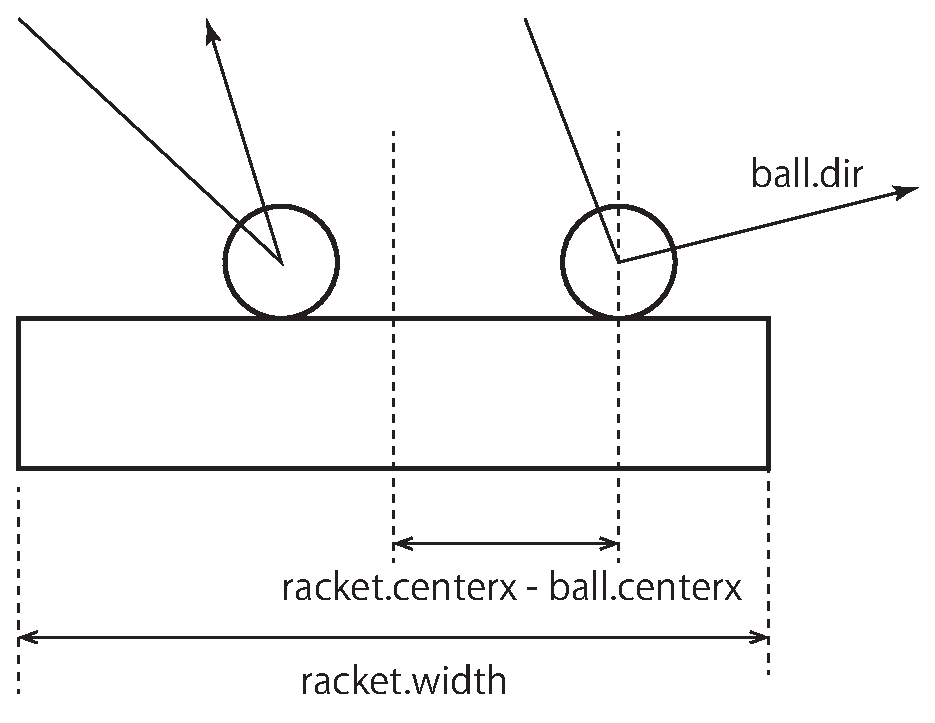
\includegraphics[width=0.4\hsize]{figures/eps/hitball.eps}
\end{center}
%干渉した場合、ballオブジェクトの進行方向を変えています

ボールがラケットに当たった位置が、ラケットの中央から左右どの程度離れているかに応じて、
ボールの反射する方向を変えるようにしています

\begin{lstlisting}[caption=Gameクラス(racketオブジェクトを追加),label=p1]
import sys
import pygame
from pygame.locals import QUIT, KEYDOWN, K_LEFT, K_RIGHT
from Ball import Ball
from Racket import Racket
from Screen import Screen

class Game():
    WHITE = (255, 255, 255)
    def __init__(self):
        pygame.init()
        self.WIDTH = 640
        self.HEIGHT = 480
        self.screen = Screen( self.WIDTH, self.HEIGHT)
        self.screen.caption("Squash game")
        self.clock = pygame.time.Clock()
        self.FPS = 30
        RED = (255,0,0)
        self.ball = Ball(self.screen.surface, color=RED)
        left = self.WIDTH//2
        top = self.HEIGHT - 50
        self.racket = Racket(self.screen.surface, left=left, top=top)
        pygame.key.set_repeat(10, 10)

    def fine(self):
        pygame.quit()
        sys.exit()

    def key_event(self):
        for event in pygame.event.get():
            if event.type == QUIT:
                self.fine()
            elif event.type == KEYDOWN:
                if event.key == K_LEFT and self.racket.left > 0:
                    self.racket.movex(-3)
                elif event.key == K_RIGHT and self.racket.right < self.WIDTH:
                    self.racket.movex(3)

    def hitted(self, racket, ball):
        if racket.colliderect( ball ):
            ball.dir = -(90+(racket.centerx-ball.centerx)/racket.width*100)

    def boundary(self, ball):
        if not (0 < ball.centerx < self.WIDTH):
            ball.dir = 180 - ball.dir
        if not (0 < ball.centery < self.HEIGHT):
            ball.dir = -ball.dir

    def start(self):
        game_over = False
        while not game_over:
            self.key_event()
            self.screen.fill( Game.WHITE )
            self.ball.draw()
            self.racket.draw()
            self.hitted( self.racket, self.ball )
            self.boundary( self.ball )
            self.ball.movexy()
            pygame.display.update()
            self.clock.tick(self.FPS)
\end{lstlisting}

\subsection{メッセージ表示のクラス:Message}

クラスの「継承」を詳しく学習するために、
メッセージのクラスは、MessageクラスとMessクラスの2段構えにしてみました\\

Messのクラスが持つ特性値(プロパティ)は次の通りです

\begin{itemize}
  \item メッセージの文字列(MESSAGE)
  \item メッセージを表示する場所(XPOS,YPOS)
  \item メッセージの色(COLOR)
  \item メッセージを描画した画面を重ねる下地の画面(surface)
  \item 文字フォント(font)と、そのサイズ(SIZE)
\end{itemize}

文字フォントのサイズは、ここでは固定値(FSIZE=80)にしています

これらの特性値はコンストラクタ(\_\_init\_\_()メソッド)で、それぞれの初期値を設定しています

コンストラクタの引数には、デフォルトの値を設定しています

これらの特性値を操作するメソッドは1つだけです

\begin{itemize}
  \item displayメソッドは、\\Fontのrenderメソッドを使ってMESSAGEを描画し、それを中心座標(XPOS、YPOS)の位置に、COLOR色でsurfaceに重ね合わせます
\end{itemize}

Messクラスを上位のクラスとして継承しているMessageクラスは、
そのコンストラクタで上位のクラスsuper()のコンストラクタを呼び出しています
Messクラスが保持しているMESSAGEプロパティ、XPOS、YPOSプロパティに値を設定しています

また、Gameクラスの中からMessageクラスのdisplay()メソッドを呼び出していますが、
実際は、継承している上位のクラスMessが保持しているdisplay()メソッドが実行されます

\begin{lstlisting}[caption=Messageクラス,label=p4]
import pygame

class Mess:
    def __init__(self, surface, size=80, color=(255,255,0)):
        self.surface = surface
        self.SIZE = size
        self.COLOR = color
        self.font = pygame.font.Font(None, size)
        self.MESSAGE = 'Hello'
        self.XPOS = self.YPOS = 0

    def display(self):
        text = self.font.render(self.MESSAGE, True, self.COLOR)
        textpos = text.get_rect()
        textpos.centerx = self.XPOS
        textpos.centery = self.YPOS
        self.surface.blit(text, textpos)

class Message( Mess ):
    def __init__(self, surface, message, xpos, ypos, size=80, color=(0,0,0)):
        super().__init__(surface, size, color)
        self.MESSAGE = message
        self.XPOS = xpos
        self.YPOS = ypos
\end{lstlisting}

\subsubsection{Gameクラスの書き換え}

Messageクラスのmsg\_goverオブジェクトを、Gameクラスのコンストラクタで生成しています

その際、メッセージ'Game Over!!'の表示色を黄色YELLOWに、表示位置をxposとyposで設定したオブジェクトにしています

コンストラクタでは、メッセージの各情報を設定しただけで、まだ表示していません

実際に表示するのは、boundary()メソッドの中でballオブジェクトがracketオブジェクトに当たらずに、
ballオブジェクトのcenteryプロパティが、screenオブジェクトのHEIGHTプロパティーを超えた時に、
msg\_goverオブジェクトが持っていたMESSAGEプロパティ'Game Over!!'を表示し、
同時に、ballオブジェクトを静止ball.stop\_ball()させています

\begin{lstlisting}[caption=Gameクラス(messageオブジェクトを追加),label=p1]
import sys
import pygame
from pygame.locals import QUIT, KEYDOWN, K_LEFT, K_RIGHT
from random import randint
from Ball import Ball
from Message import Message
from Racket import Racket
from Screen import Screen

class Game():
    WHITE = (255, 255, 255)
    def __init__(self):
        pygame.init()
        self.WIDTH = 640
        self.HEIGHT = 480
        self.screen = Screen( self.WIDTH, self.HEIGHT)
        self.screen.caption("Squash game")
        self.clock = pygame.time.Clock()
        self.FPS = 30
        RED = (255,0,0)
        START = ( randint(0,self.WIDTH-1),0 )
        self.ball = Ball( self.screen.surface, color=RED, start=START )
        left = self.WIDTH//2
        top = self.HEIGHT - 50
        self.racket = Racket(self.screen.surface, left=left, top=top)
        xpos = left
        ypos = self.HEIGHT//2
        YELLOW = (255,255,0)
        self.msg_gover = Message( self.screen.surface, 'Game Over!!',\
                                  xpos, ypos, color=YELLOW )
        pygame.key.set_repeat(10, 10)

    def fine(self):
        pygame.quit()
        sys.exit()

    def key_event(self):
        for event in pygame.event.get():
            if event.type == QUIT:
                self.fine()
            elif event.type == KEYDOWN:
                if event.key == K_LEFT and self.racket.left > 0:
                    self.racket.movex(-3)
                elif event.key == K_RIGHT and self.racket.right < self.WIDTH:
                    self.racket.movex(3)

    def hitted(self, racket, ball):
        if racket.colliderect( ball ):
            ball.dir = -(90+(racket.centerx-ball.centerx)/racket.width*100)

    def boundary(self, ball):
        if not (0 < ball.centerx < self.WIDTH):
            ball.dir = 180 - ball.dir
        if ball.centery < 0:
            ball.dir = -ball.dir
        if self.HEIGHT < ball.centery:
            ball.stop_ball()
            self.msg_gover.display()

    def start(self):
        game_over = False
        while not game_over:
            self.key_event()
            self.screen.fill( Game.WHITE )
            self.ball.draw()
            self.racket.draw()
            self.hitted( self.racket, self.ball )
            self.boundary( self.ball )
            self.ball.movexy()
            pygame.display.update()
            self.clock.tick(self.FPS)
\end{lstlisting}

%\lstinputlisting[caption=Squashゲームの完成,label=squash]{squashobj1.py}

\chapter{ブロック崩しゲーム}

ブロック崩しゲームは、スカッシュ・ゲームに、
ブロック部分のオブジェクトを追加して作ります

\begin{center}
  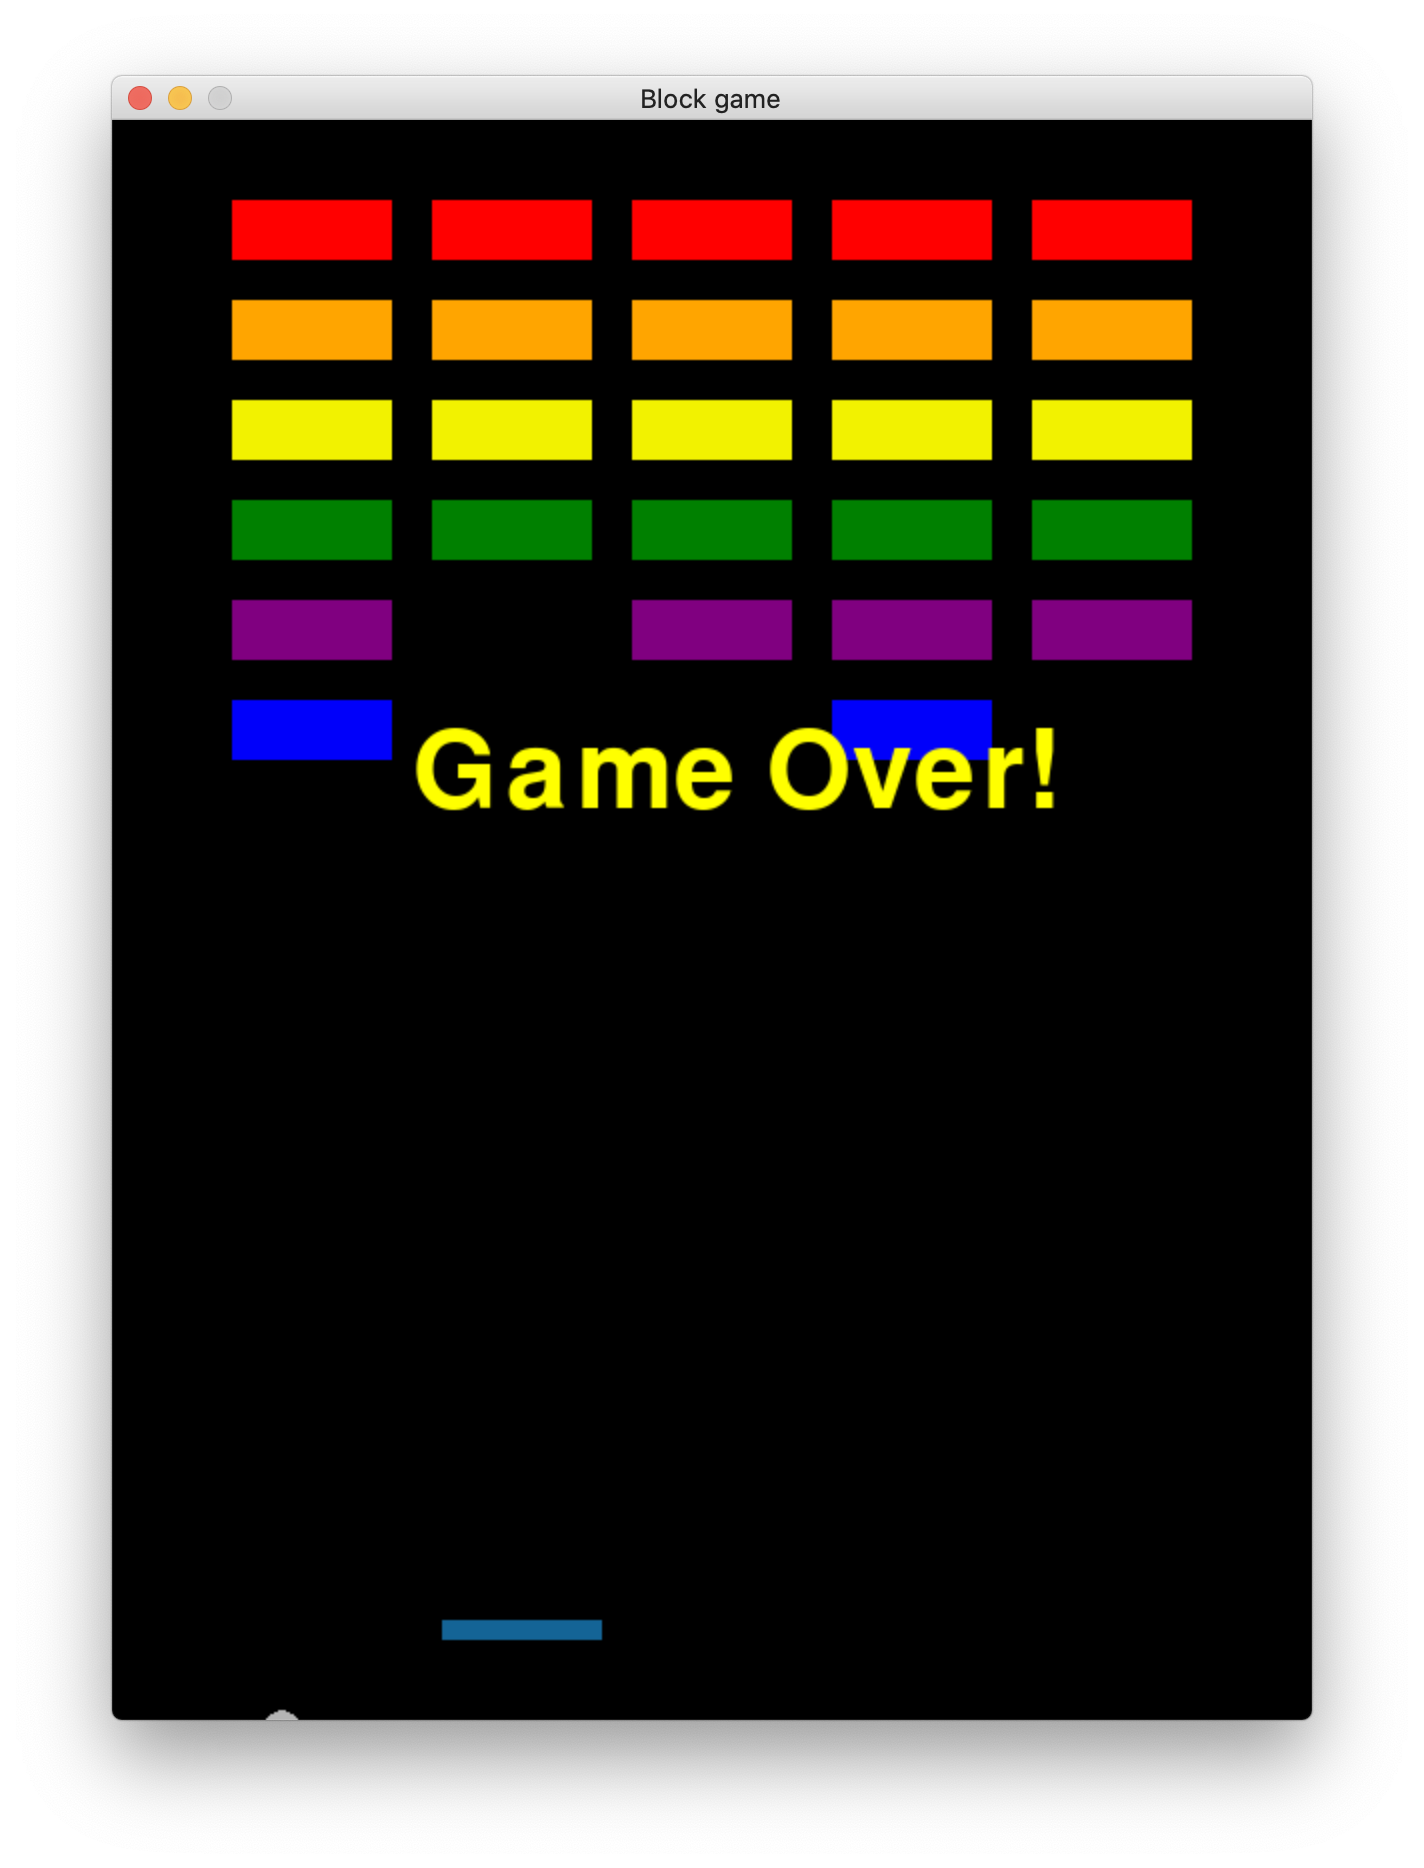
\includegraphics[width=0.45\hsize]{figures/eps/blockgame.eps}
\end{center}

\subsection{ブロッククラス:BlockとBlocks}

ブロック部分の全体をBlocksクラス、その中の個々のブロックをBlockクラスで定義します

BlockクラスはRectクラスを継承させることとし、そのプロパティは次の通りです

\begin{itemize}
  \item ブロックの左座標(left)
  \item ブロックの上座標(top)
  \item ブロックの幅(width)
  \item ブロックの高さ(height)
  \item ブロックの色(COLOR)
  \item ブロックを配置する場所(surface)
\end{itemize}

ブロックをdraw.rect()で描画するためのメソッドdrawを持たせています

\begin{lstlisting}[caption=Class BlockとBlocks,label=p4]
import pygame
from pygame.locals import Rect

class Block(Rect):
    def __init__(self, surface, color, rect):
        self.surface = surface
        self.COLOR = color
        self.left = rect[0]
        self.top = rect[1]
        self.width = rect[2]
        self.height = rect[3]

    def draw(self):
        pygame.draw.rect(self.surface, self.COLOR, self)

class Blocks():
    def __init__(self, surface):
        self.surface = surface
        WIDTH = 80
        HEIGHT = 30
        COLORS = [(255,0,0), (255,165,0), (242,242,0),\
                       (0,128,0), (128,0,128), (0,0,250)]
        self.blocks = []
        for ypos, color in enumerate( COLORS, start=0):
            for xpos in range(0, 5):
                self.blocks.append( Block(self.surface, color,\
                            Rect(xpos*100+60, ypos*50+40, WIDTH, HEIGHT)) )

    def draw(self):
        for block in self.blocks:
            block.draw()
\end{lstlisting}

Blockオブジェクトを6行5列に並べるクラスをBlocksクラスとして定義します

Blocksクラスの主なプロパティは、Blockオブジェクトのリストです

\begin{center}
  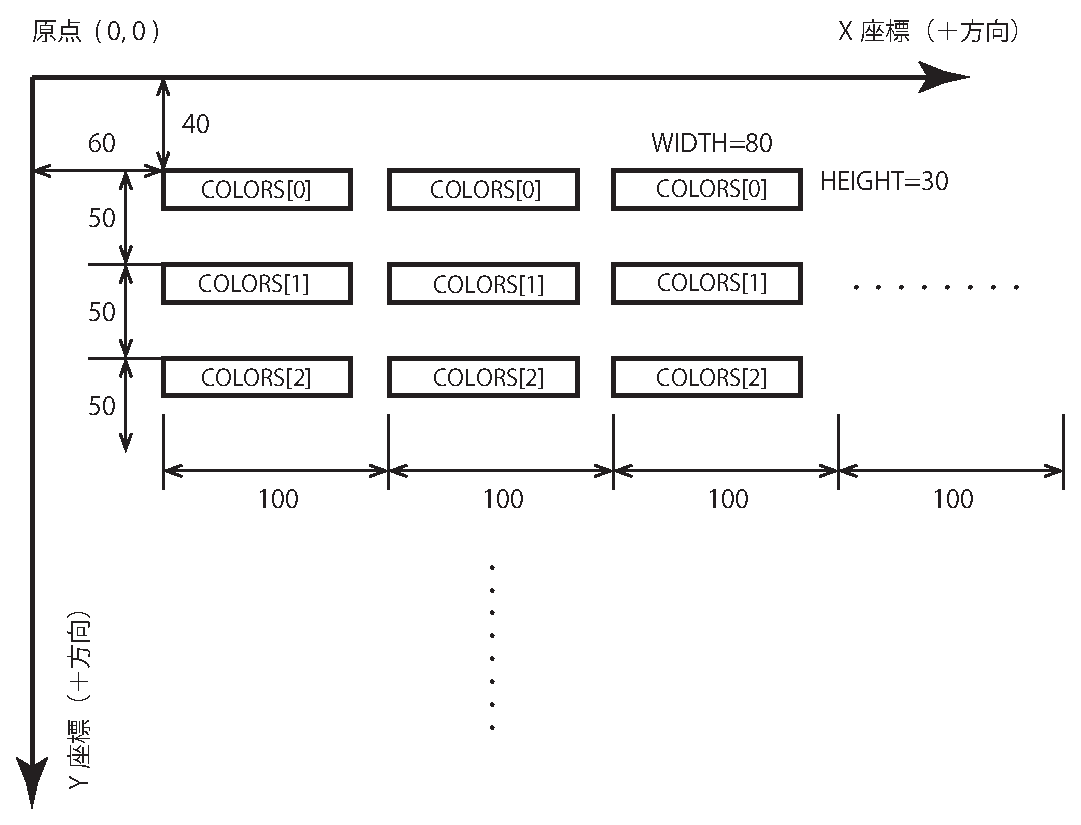
\includegraphics[width=0.6\hsize]{figures/eps/blocks.eps}
\end{center}

\begin{itemize}
  \item 6行5列のBlockオブジェクトのリストを持っています(blocks)
\end{itemize}

メソッドとして、次のようなものを用意することが考えられます

\begin{itemize}
  %\item get\_blocksメソッドは、\\6行5列のBlockのオブジェクトのリストを返します
  %\item set\_blocksメソッドは、\\引数で受け取ったblocksリストを、自分のBlocksオブジェクト内のblocksリストに保存します
  \item drawメソッド:6行5列のブロックオブジェクトを描画します
\end{itemize}

オブジェクトの中のプロパティ(特性)の値を返すメソッドは「ゲッター(getter)」と呼ばれます

オブジェクトの中のプロパティ(特性)に値を設定するメソッドは「セッター(setter)」と呼ばれます

ゲッターの関数名は「get云々」、セッターの関数名は「set云々」という書き方をします

ゲッターやセッターを用意しようとするなら、次のメソッドを用意する必要があります

\begin{itemize}
  \item get\_blocksメソッド:6行5列のBlockのオブジェクトのリストを返します
  \item set\_blocksメソッド:引数で受け取ったリストを、Blocksオブジェクト内の変数に保存します
  %\item drawメソッドは、\\6行5列のブロックオブジェクトを描画します
\end{itemize}

しかし、「Effective Python」という書籍の第6章の項目44では、
「getメソッドやsetメソッドは使わずに属性をそのまま使う」のが良い(→その方がPythonicな書き方である)との記述があります

JavaやC++言語では、セッターやゲッターは通常書いてしまうものですが、Pythonでは推奨されていない(どうしてもPythonで必要なら、メタクラスの書き方を使え)ということです

セッターやゲッターを使わないこととして、このクラスのメソッドはdrawメソッドだけにします

\subsubsection{Gameクラスの書き換え}

ブロック崩しでは、ブロックを全て打ち崩した場合、'Cleared!!'と表示させたいと思います

また、ブロックを1つ消すごとに10ポイントを加算して、それが画面上部に表示されるようにします

Blocksクラスのオブジェクトであるblocksの中に保持しているblocksという名称のプロパティですが、
これはBlockクラスのオブジェクトであるblockのリストでしたから、そのリストの長さをlen()関数で
調べて、長さがゼロになったなら全てのブロックを崩してしまったと判断して、'Cleared!!'と表示しています

\begin{lstlisting}[caption=Gameクラス(blocksオブジェクトを追加),label=p1]
import sys
import pygame
from pygame.locals import QUIT, KEYDOWN, K_LEFT, K_RIGHT
from random import randint
from Ball import Ball
from Message import Message
from Racket import Racket
from Screen import Screen
from Blocks import Blocks

class Game():
    BLACK = (0, 0, 0)
    def __init__(self):
        pygame.init()
        self.WIDTH = 600
        self.HEIGHT = 800
        self.screen = Screen( self.WIDTH, self.HEIGHT)
        self.screen.caption("Block game")
        self.clock = pygame.time.Clock()
        self.FPS = 30
        RED = (255,0,0)
        START = ( randint(0,self.WIDTH-1), self.HEIGHT//2 )
        self.red_ball = Ball( self.screen.surface, color=RED, start=START )
        left = self.WIDTH//2
        top = self.HEIGHT - 50
        self.racket = Racket(self.screen.surface, left=left, top=top )
        xpos = left
        ypos = self.HEIGHT//2
        YELLOW = (255,255,0)
        self.msg_gover = Message( self.screen.surface, 'Game Over!!',\
                                  xpos, ypos, color=YELLOW )
        self.msg_clear = Message( self.screen.surface, 'Clear!!',\
                                  xpos, ypos, color=YELLOW)
        ypos = 20
        self.msg_point = Message( self.screen.surface, 'Point'+'=0',\
                                  xpos, ypos, size=30, color=YELLOW )
        self.blocks = Blocks( self.screen.surface )
        self.point = 0
        pygame.key.set_repeat(10, 10)

    def fine(self):
        pygame.quit()
        sys.exit()

    def key_event(self, racket):
        for event in pygame.event.get():
            if event.type == QUIT:
                self.fine()
            elif event.type == KEYDOWN:
                if event.key == K_LEFT and racket.left > 0:
                    racket.movex(-3)
                elif event.key == K_RIGHT and racket.right < self.WIDTH:
                    racket.movex(3)

    def cleared(self, blocks, ball):
        if len(blocks.blocks) == 0:
            ball.stop_ball()
            self.msg_clear.display()

    def clashed(self, blocks, ball):
        b0 = blocks.blocks
        b1 = [x for x in b0 if not x.colliderect(ball)]
        if len(b0) != len(b1):
            blocks.blocks = b1
            ball.dir = -ball.dir
            self.point += 10
            self.msg_point.MESSAGE = 'Point=' + str(self.point)

    def hitted(self, racket, ball):
        if racket.colliderect( ball ):
            ball.dir = -(90 + (racket.centerx-ball.centerx)/racket.width*100)

    def boundary(self, ball):
        if not (0 < ball.centerx < self.WIDTH):
            ball.dir = 180 - ball.dir
        if ball.centery < 0:
            ball.dir = -ball.dir
        if self.HEIGHT < ball.centery:
            ball.stop_ball()
            self.msg_gover.display()

    def draw(self):
        self.screen.fill( Game.BLACK )
        self.blocks.draw()
        self.red_ball.draw()
        self.racket.draw()

    def start(self):
        game_over = False
        while not game_over:
            self.key_event( self.racket )
            self.draw()
            self.cleared( self.blocks, self.red_ball )
            self.clashed( self.blocks, self.red_ball )
            self.hitted( self.racket, self.red_ball )
            self.boundary( self.red_ball )
            self.msg_point.display()
            self.red_ball.movexy()
            pygame.display.update()
            self.clock.tick(self.FPS)
\end{lstlisting}

\subsubsection{GameクラスにScreenクラスを継承させる}

GameクラスがScreenクラスを継承することによって、GameクラスはScreenクラスが持っているプロパティとメソッドを、
あたかも自分のクラスのもののように使うことができます

これまで、self.screen.surface と書いていた部分が何カ所かありました

これは、Screenクラスのオブジェクトであるscreenが保持しているsurfaceという名前のプロパティだという意味なのですが、
この部分を self.surface として、あたかもGameクラスのオブジェクトがsurfaceというプロパティを持っているかのように記述できることになります

また、surfaceオブジェクトの幅WIDTHと高さHEIGHTについても、
Gameの中で定義しなくてもScreenクラスのプロパティを、self.WIDTHやself.HEIGHTとして参照できます

Screenクラスのコンストラクタを、super().\_\_init\_\_( 引数 ) という形で呼び出している点にも注目しましょう

\begin{lstlisting}[caption=Gameクラス(Screenクラスを継承),label=p2]
import sys
import pygame
from pygame.locals import QUIT, KEYDOWN, K_LEFT, K_RIGHT
from random import randint
from Ball import Ball
from Message import Message
from Racket import Racket
from Screen import Screen
from Blocks import Blocks

class Game( Screen ):
    BLACK = (0, 0, 0)
    def __init__(self):
        pygame.init()
        super().__init__( width=600, height=800 )
        self.caption("Block game")
        self.clock = pygame.time.Clock()
        self.FPS = 30
        RED = (255,0,0)
        START = ( randint(0,self.WIDTH-1), self.HEIGHT//2 )
        self.red_ball = Ball( self.surface, color=RED, start=START )
        left = self.WIDTH//2
        top = self.HEIGHT - 50
        self.racket = Racket(self.surface, left=left, top=top )
        xpos = left
        ypos = self.HEIGHT//2
        YELLOW = (255,255,0)
        self.msg_gover = Message( self.surface, 'Game Over!!', xpos, ypos, color=YELLOW )
        self.msg_clear = Message( self.surface, 'Clear!!', xpos, ypos, color=YELLOW)
        ypos = 20
        self.msg_point = Message( self.surface, 'Point'+'=0', xpos, ypos, size=30, color=YELLOW )
        self.blocks = Blocks( self.surface )
        self.point = 0
        pygame.key.set_repeat(10, 10)

    def fine(self):
        pygame.quit()
        sys.exit()

    def key_event(self, racket):
        for event in pygame.event.get():
            if event.type == QUIT:
                self.fine()
            elif event.type == KEYDOWN:
                if event.key == K_LEFT and racket.left > 0:
                    racket.movex(-3)
                elif event.key == K_RIGHT and racket.right < self.WIDTH:
                    racket.movex(3)

    def cleared(self, blocks, ball):
        if len(blocks.blocks) == 0:
            ball.stop_ball()
            self.msg_clear.display()

    def clashed(self, blocks, ball):
        b0 = blocks.blocks
        b1 = [x for x in b0 if not x.colliderect(ball)]
        if len(b0) != len(b1):
            blocks.blocks = b1
            ball.dir = -ball.dir
            self.point += 10
            self.msg_point.MESSAGE = 'Point=' + str(self.point)

    def hitted(self, racket, ball):
        if racket.colliderect( ball ):
            ball.dir = -(90 + (racket.centerx-ball.centerx)/racket.width*100)

    def boundary(self, ball):
        if not (0 < ball.centerx < self.WIDTH):
            ball.dir = 180 - ball.dir
        if ball.centery < 0:
            ball.dir = -ball.dir
        if self.HEIGHT < ball.centery:
            ball.stop_ball()
            self.msg_gover.display()

    def draw(self):
        self.fill( Game.BLACK )
        self.blocks.draw()
        self.red_ball.draw()
        self.racket.draw()

    def start(self):
        game_over = False
        while not game_over:
            self.key_event( self.racket )
            self.draw()
            self.cleared( self.blocks, self.red_ball )
            self.clashed( self.blocks, self.red_ball )
            self.hitted( self.racket, self.red_ball )
            self.boundary( self.red_ball )
            self.msg_point.display()
            self.red_ball.movexy()
            pygame.display.update()
            self.clock.tick(self.FPS)
\end{lstlisting}

\newpage

【演習】
\begin{enumerate}
  \item[(1)] ゲームをClearできずにGame overとなった場合、画面の背景色を変えて(例えば白黒点滅させて)終わるような演出を考えてみよう
  \item[(2)] Ballクラスに、「ボールの移動スピードを変えるメソッド」を追加し、\\
  得点(取得ポイント)が増えるのに従って、ボールのスピードが速くなるように直してみよう
  \item[(3)] Ballクラスに、「ボールの半径を変えるメソッド」を追加し、\\
  得点(取得ポイント)が増えるのに従って、ボールの半径が小さくなるように直してみよう
  \item[(4)] Ballクラスに、「ボールの色を変えるメソッド」を追加し、\\
  ラケットで跳ね返すタイミングで、乱数によってボールの色を変えるように演出してみよう
  \item[(5)] Racketクラスに、「ラケットの色を変えるメソッド」を追加し、\\
  ボールをラケットで打ち返す瞬間、ラケットの色、そしてボールの色や半径を一時的に変えて(点滅させて)元に戻すなどの演出を考えてみよう
  \item[(6)] Racketクラスに、「ラケットの横幅を変えるメソッド」を追加し、\\
  得点(取得ポイント)が増えるのに従って、ラケットの幅が短くなっていくように直してみよう
  \item[(7)] 得点(取得ポイント)が増えるのに従って、ラケットを移動させる単位移動ステップ数が少なくなるように直してみよう
  \item[(8)] blue\_ball オブジェクトを追加して、
  ゆっくり移動するblue\_ballと速く移動するred\_ballの2個を、ラケットで跳ね返しながらゲームできるように直してみよう
  \item[(9)] 得点(取得ポイント)がある点数以上になったら、2個目のボールが出現するように直してみよう
  \item[(10)] 2つのボールの干渉を検出できるようにして、衝突したときの両方のボールの動作を考えてみよう
  \item[(11)] 通常スピードで動くred\_ballの1個だけで行うStage1をClearできたなら、
  Stage2では2個目のボールが追加された状態でゲームが再開されるように直してみよう
  \item[(12)] 2個のボールでゲームをスタートし、途中ブロックの数が特定の値になっている間に、
  2個のボールを衝突させた場合に、2個のボールが合体して1個のボールでゲームを進行できるように直してみよう
  (ボールが合体するときには、ボールの色や半径を一時的に変化させる演出を考えてみよう)
  \item[(13)] ブロックの数が最後の1個になった時に、にわかに数個のボールが出現するようにする、、と、、、、Clearできないゲームになるかも
  \item[(14)] 実は、pygameでは音を出すこともできます\\
  ラケットにボールが当たったときの音やブロックにボールが当たったときの音、Game overのときの音やゲームをClearできたときの音など、
  さらにはBGMなどの演出も考えられますので、調べて試してみると楽しいゲームになるかもしれませんね
\end{enumerate}

\chapter{スペース インベーダ ゲーム}

\section{スペース インベーダ ゲーム}

\begin{center}
  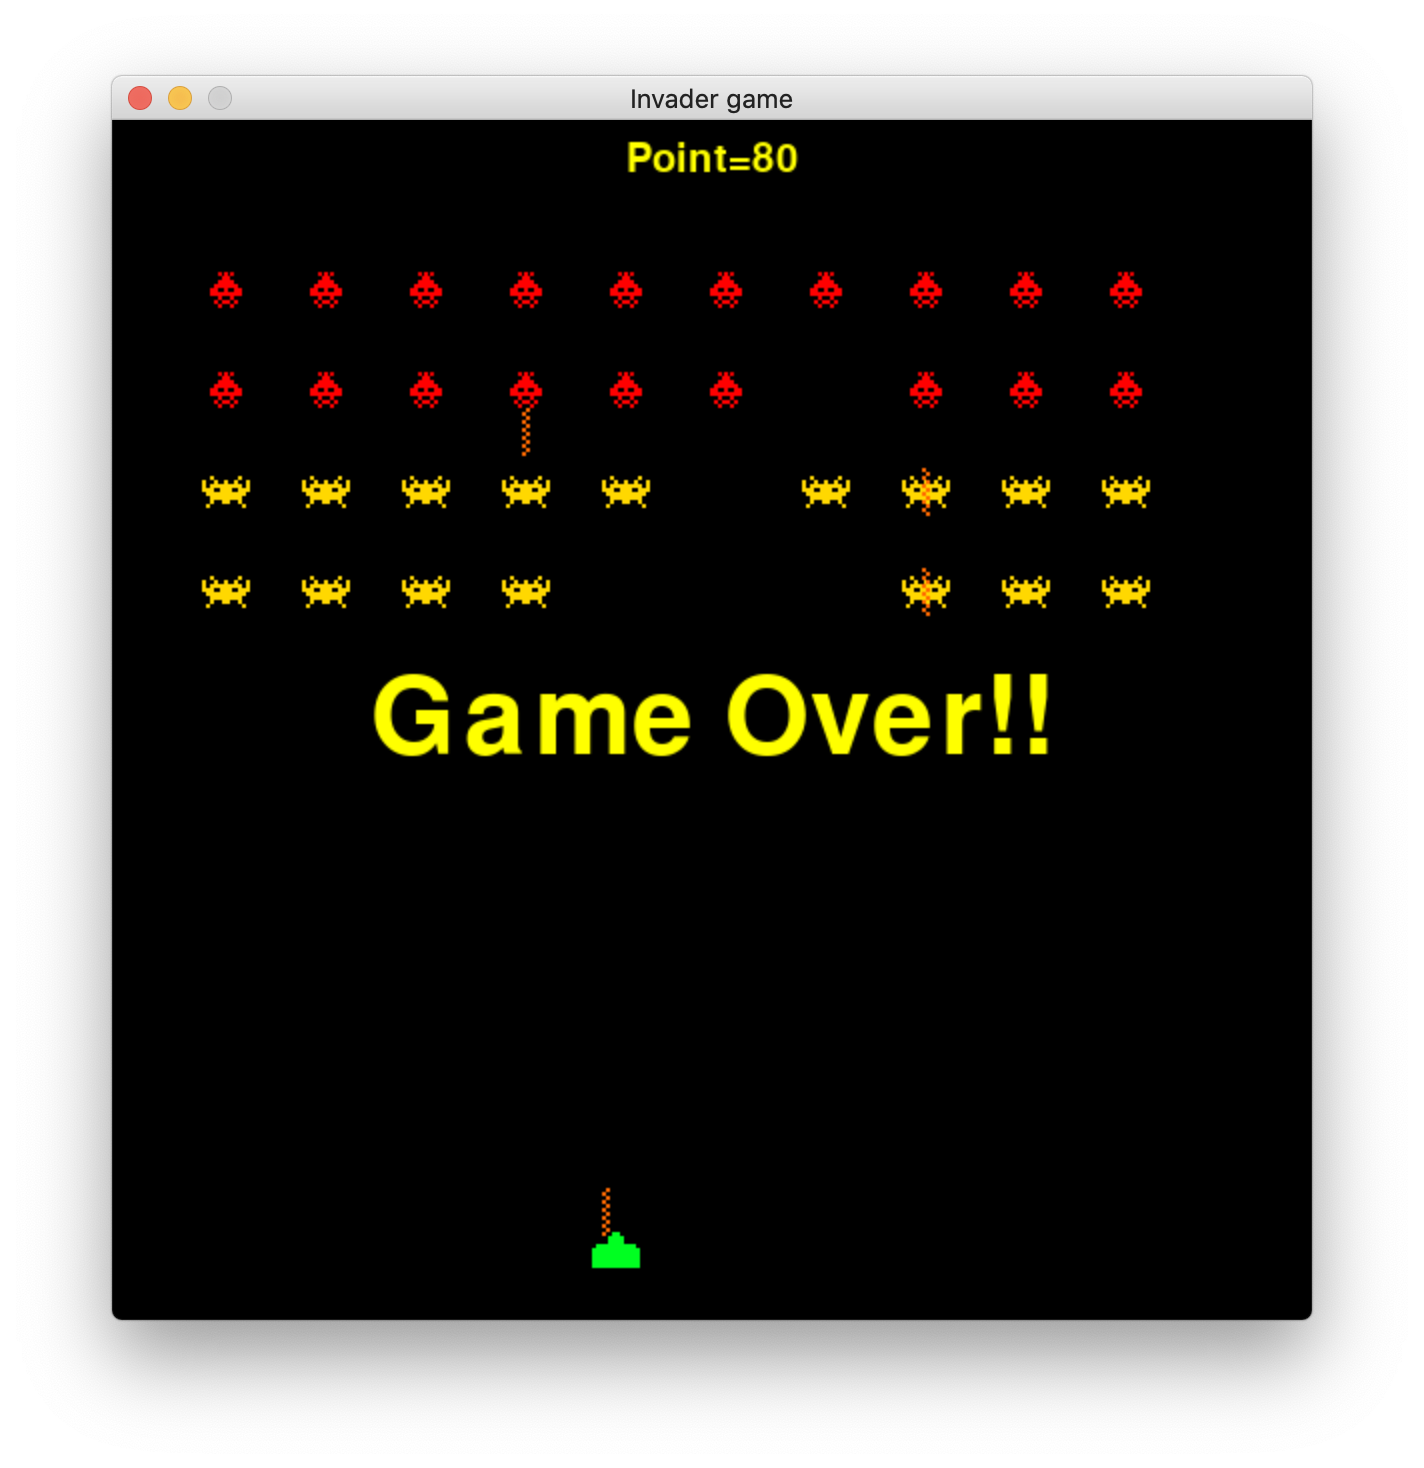
\includegraphics[width=0.5\hsize]{figures/eps/invadergame.eps}
\end{center}

\subsection{画面のクラス:Screen}

\begin{lstlisting}[caption=Class Screen,label=p002]
import pygame

class Screen:
    def __init__(self, width=600, height=600):
        self.WIDTH = width
        self.HEIGHT = height
        self.SIZE = (width, height)
        self.surface = pygame.display.set_mode(self.SIZE)

    def fill(self, color=(255, 255, 255)):
        self.surface.fill(color)

    def caption(self, str):
        pygame.display.set_caption(str)
\end{lstlisting}

\subsection{ゲームの進行を司るクラス:Game}

\begin{lstlisting}[caption=Class Game,label=p001]
import sys
import pygame
from pygame.locals import QUIT, KEYDOWN, K_RIGHT, K_LEFT, K_SPACE
from Screen import Screen

class Game( Screen ):
    BLACK = (0, 0, 0)
    def __init__(self):
        pygame.init()
        super().__init__(width=600, height=800)
        self.caption("Invader game")
        self.clock = pygame.time.Clock()
        self.FPS = 30

    def fine(self):
        pygame.quit()
        sys.exit()

    def key_event(self):
        for event in pygame.event.get():
            if event.type == QUIT:
                self.fine()

    def start(self):
        self.gameover = False
        while True:
            self.key_event()
            self.fill( Game.BLACK )
            # ここにゲームの流れを記述します
            pygame.display.update()
            self.clock.tick(self.FPS)
\end{lstlisting}

GameクラスはScreenクラスを継承するようにします

クラス変数Game.BLACKを用意しています

なお、main.pyを次のようにします

\begin{lstlisting}[caption=main.py,label=p000]
from Game import Game

if __name__ == '__main__':
    game = Game()
    game.start()
\end{lstlisting}

\subsection{画像データを管理するクラス:Images}

Ship以外の画像は画面に動きをつけるため、2つの画像を交互に描画する事を想定しています

このクラスは、他のクラス(ビーム、爆弾、エイリアン、自機)の上位クラスとして使います

それぞれ下位クラスがコンストラクタで初期化される際に呼び出され、2つの画像を読み込んでimages[0]とimages[1]に納めています

なお、画像データは全て24x24ピクセルのサイズを想定しています

%\newpage

\begin{lstlisting}[caption=Class Images,label=p003]
import pygame
from pygame.locals import Rect

class Images( Rect ):
    def __init__(self, surface, fname0, fname1):
        self.surface = surface
        self.count = 0
        width = height = 24
        self.size = (width, height)
        strip0 = pygame.image.load(fname0 + '.png')
        strip1 = pygame.image.load(fname1 + '.png')
        IMGS = (pygame.Surface(self.size, pygame.SRCALPHA), \
                pygame.Surface(self.size, pygame.SRCALPHA))
        top = left = 0
        rect = Rect(left, top, width, height)
        IMGS[0].blit( strip0, (0,0), rect )
        IMGS[1].blit( strip1, (0,0), rect )
        self.images=[IMGS[0], IMGS[1]]

    def move(self, delx, dely):
        self.count += 1
        self.move_ip(delx, dely)

    def draw(self):
        self.count = self.count % 2
        image = self.images[ self.count ]
        self.surface.blit(image, self.topleft)
\end{lstlisting}

\subsection{自機のクラス:Ship}

\begin{center}
  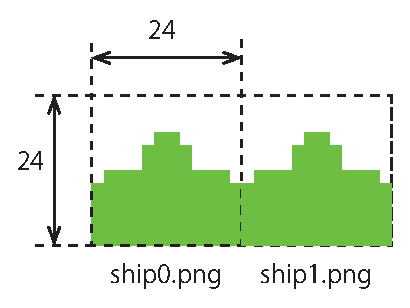
\includegraphics[width=0.3\hsize]{figures/eps/ship0.eps}
\end{center}

ship0.pngとship1.pngに同じ画像データを使うと、Shipの表示は変わらないまま移動させられます

\begin{lstlisting}[caption=Class Ship,label=p004]
from Images import Images

class Ship( Images ):
    def __init__(self, surface):
        super().__init__(surface, 'ship0', 'ship1')
        self.surface = surface
        self.left = surface.get_rect().width//2
        self.top = surface.get_rect().height - 50
        self.width = self.height = 24

    def movex(self, delx):
        self.move(delx, 0)
\end{lstlisting}

movex()メソッドの引数delxは、自機の移動速度です

\subsubsection{Gameクラスの書き換え}

Gameクラスのコンストラクタで、Shipクラスのオブジェクトを生成します

KEYDOWNイベントを取得し、左右方向の矢印でshipオブジェクトの位置を左右に動かします

drawメソッドによって、shipオブジェクトを描画します

\begin{lstlisting}[caption=Gameクラス(shipオブジェクトを追加),label=p001-1]
import sys
import pygame
from pygame.locals import QUIT, KEYDOWN, K_RIGHT, K_LEFT, K_SPACE
from Screen import Screen
from Ship import Ship

class Game( Screen ):
    BLACK = (0, 0, 0)
    def __init__(self):
        pygame.init()
            ・
            ここは変わらず
            ・
        self.FPS = 30
        self.ship = Ship( self.surface )  # Shipクラスのオブジェクト生成を追加

    def fine(self):
        pygame.quit()
        sys.exit()

    def key_event(self, ship):  # ship を引数に追加
        for event in pygame.event.get():
            if event.type == QUIT:
                self.fine()
            elif event.type == KEYDOWN:    # キーボードイベントの取得を追加
                if event.key == K_LEFT and ship.left > 0:
                    ship.movex(-5)    # shipオブジェクトの左右の動きを追加
                elif event.key == K_RIGHT and ship.right < self.WIDTH:
                    ship.movex(5)

    def start(self):
        self.gameover = False
        while True:
            self.key_event( self.ship )   # self.ship を引数に追加
            self.fill( Game.BLACK )
            #
            self.ship.draw()         # shipオブジェクトの描画を追加
            #
            pygame.display.update()
            self.clock.tick(self.FPS)
\end{lstlisting}

【演習】ここまでのプログラムを実行してみよう\\(自機Shipが左右の矢印キーのイベントで移動できることを確認しよう)

\subsection{ビームのクラス:Beam}

\begin{center}
  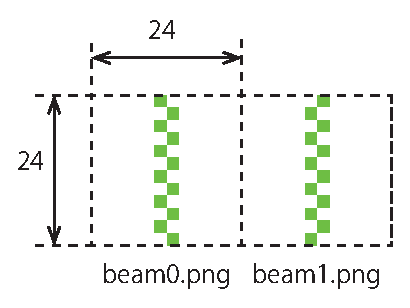
\includegraphics[width=0.3\hsize]{figures/eps/beam0.eps}
  %\includegraphics[width=0.1\hsize]{beam1.png}
\end{center}

beam0.pngとbeam1.pngを交互に表示して、動きを表します

ビームのオブジェクトは、画面の中に1個だけです

movey()メソッドのデフォルト引数(dely=-15)は、ビームオブジェクトの移動速度です

\begin{lstlisting}[caption=Class Beam,label=p005]
from Images import Images

class Beam( Images ):
    def __init__(self, surface):
        super().__init__(surface, 'beam0', 'beam1')
        self.surface = surface

    def movey(self, dely=-15):
        self.move(0, dely)
\end{lstlisting}

\subsubsection{Gameクラスの書き換え}

Beamクラスのオブジェクトを、Gameクラスのコンストラクタの中で生成します

キーボードイベントでスペースキーの押下(K\_SPACE)を検出したとき、
beamオブジェクトの下端(beam.bottom)の値が負になっている($<$0)なら、
beamオブジェクトは画面の外にいるので、ビームを、自機(ship)から発射させることができます(beam.center=ship.center)

その後ゲームの反復ループ内で、beamオブジェクトを上方向(yが減る方向)に移動させ描画します

beamオブジェクトは、そのうち画面の上端より上(beam.bottom $<$ 0)に行って、画面から消えます

画面から消えたら、再び自機から発射することが可能になります

\begin{lstlisting}[caption=Gameクラス(beamオブジェクトを追加),label=p001-2]
import sys
import pygame
from pygame.locals import QUIT, KEYDOWN, K_RIGHT, K_LEFT, K_SPACE
from Screen import Screen
from Ship import Ship
from Beam import Beam

class Game( Screen ):
    BLACK = (0, 0, 0)
    def __init__(self):
        pygame.init()
            ・
            ここは変わらず
            ・
        self.ship = Ship( self.surface )
        self.beam = Beam( self.surface )   # beamオブジェクト生成を追加

    def fine(self):
            ・
            変わらず
            ・
    def key_event(self, ship, beam):  # beam を引数に追加
        for event in pygame.event.get():
            if event.type == QUIT:
                self.fine()
            elif event.type == KEYDOWN:
                if event.key == K_LEFT and ship.left > 0:
                      ・
                    変わらず
                      ・
                elif event.key == K_SPACE and beam.bottom < 0:
                    # beamの位置をshipの位置と一緒にして、そこからbeamを発射
                    beam.center = ship.center

    def start(self):
        self.gameover = False
        while True:
            self.key_event( self.ship, self.beam )  # self.beam を引数に追加
            self.fill( Game.BLACK )
            #
            self.ship.draw()
            self.beam.movey()   # 追加:beam を動かして
            self.beam.draw()    # 追加:beam を描画
            #
            pygame.display.update()
            self.clock.tick(self.FPS)
\end{lstlisting}

【演習】ここまでのプログラムを実行してみよう\\
(スペースキーの押下によってShipの位置からbeamが発せられることを確認しよう)

\subsection{エイリアンのクラス:AlienとAliens}

\begin{table}[htb]
\begin{center}
    \begin{tabular}{cc}
    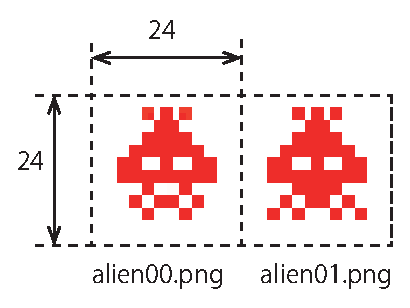
\includegraphics[width=0.3\hsize]{figures/eps/alien0.eps} & 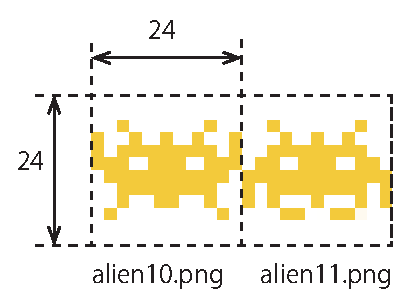
\includegraphics[width=0.3\hsize]{figures/eps/alien1.eps}
  \end{tabular}
\end{center}
\end{table}

alien00.pngとalien01.pngをエイリアン群の奥に配置し、
alien10.pngとalien11.pngをエイリアン群の手前に配置します

エイリアンの一群をAliensクラスで管理し、個々のエイリアンはAlienクラスで定義しています

エイリアンのオブジェクトを生成するときに、alien = Alien(surface, rect, 0, (4-ypos)*10)、
などとして、最後の引数でそれぞれのオブジェクト毎に得点を保持させています。

自機Shipからスペースバーによって発射されたBeamが、Alienのオブジェクトに当たったとき、
そのAlienが保持していた得点を獲得したポイントとして加算していくようにします。

%\newpage

\begin{lstlisting}[caption=Class Aliens,label=p006]
from Images import Images
from pygame.locals import Rect

class Alien(Images):
    def __init__(self, surface, rect0, img, point):
        if img==0:
            super().__init__(surface, 'alien00', 'alien01')
        else:
            super().__init__(surface, 'alien10', 'alien11')
        self.point = point
        self.left = rect0.left
        self.top = rect0.top
        self.width = rect0.width
        self.height = rect0.height

class Aliens(Alien):
    def __init__(self, surface):
        self. surface = surface
        self.counter = 0
        self.move_interval = 20
        self.move_steps = -5
        self.aliens = []
        for ypos in range(4):
            for xpos in range(10):
                left = 100 + xpos * 50
                top =  50 + ypos * 50
                width = height = 24
                rect = Rect(left, top, width, height)
                if ypos<2:
                    alien = Alien(surface, rect, 0, (4-ypos)*10)
                else:
                    alien = Alien(surface, rect, 1, (4-ypos)*10)
                self.aliens.append( alien )
        self.area = self.aliens[0].copy()
        self.stopflag = False

    def movexy(self):
        if self.stopflag:
            return
        self.area = self.aliens[0].copy()
        for alien in self.aliens:
            self.area.union_ip( alien )
        self.counter += 1
        if self.counter % self.move_interval == 0:
            movey = 0
            delx =  abs(self.move_steps)
            if self.area.left<delx or\
                        self.area.right>self.surface.get_rect().width-delx:
                movey = 24
                self.move_steps = -self.move_steps
                rate = 1.0 - (self.area.top / self.surface.get_rect().height)
                val = int(self.move_interval * rate)
                self.move_interval = 1 if val<=1 else val
            movex = self.move_steps
            for alien in self.aliens:
                alien.move(movex, movey)

    def draw(self):
        for alien in self.aliens:
            alien.draw()

    def stop(self):
        self.stopflag = True
\end{lstlisting}

\begin{table}[htb]
\begin{center}
    \begin{tabular}{c}
    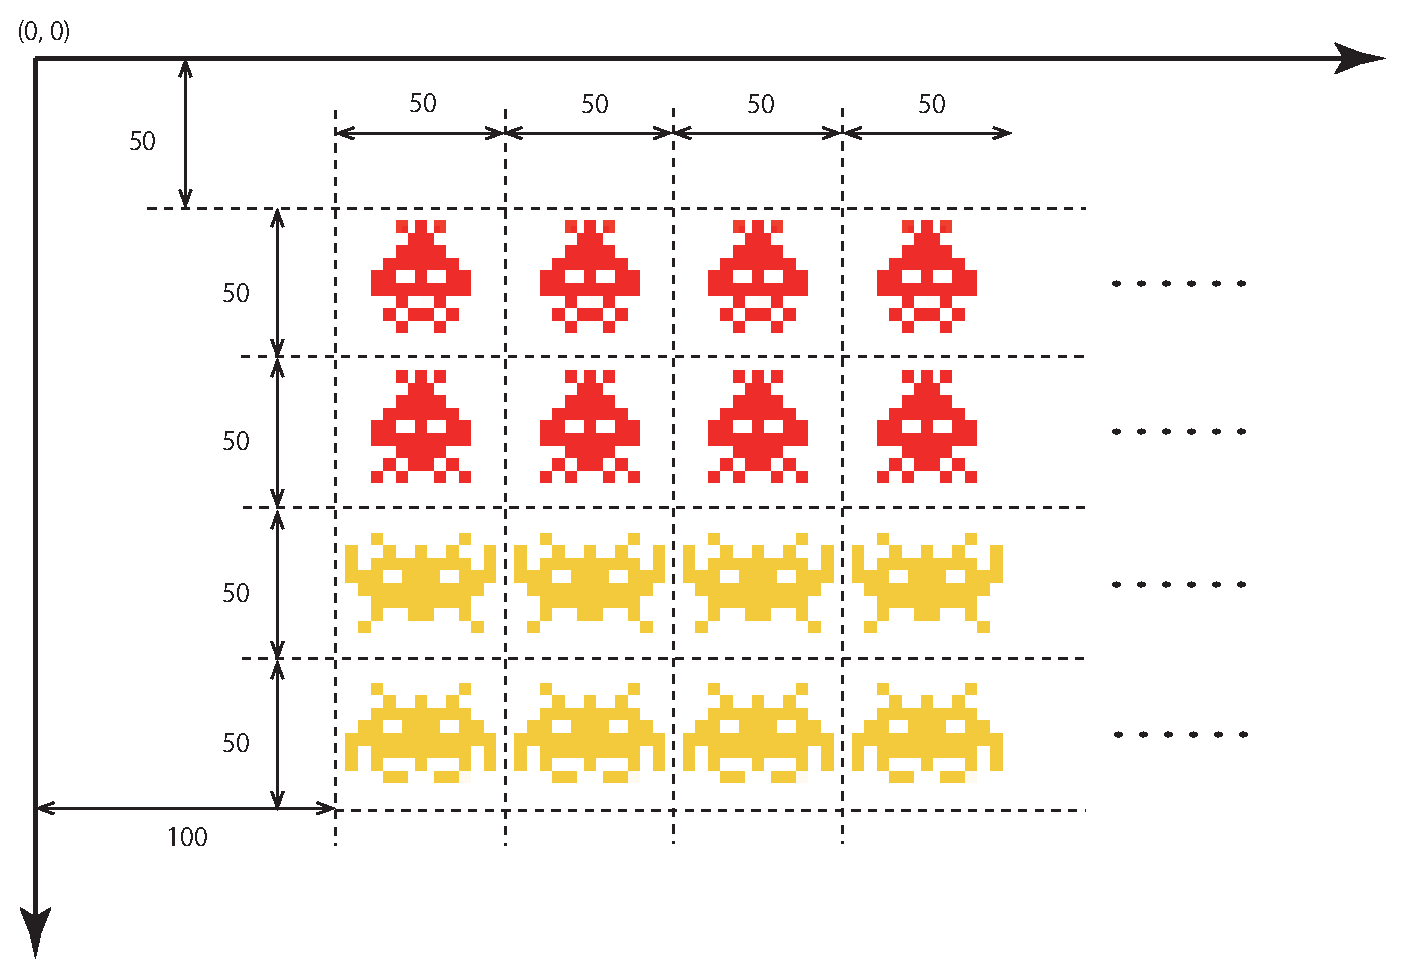
\includegraphics[width=0.7\hsize]{figures/eps/aliens.eps}
  \end{tabular}
\end{center}
\end{table}

movexy()メソッドが呼ばれる度に、counterをインクリメントして、
counterの値がmove\_intervalに設定した回数に達したとき
(counterをmove\_intervalで割った余りがゼロになったとき)に、
エイリアンをmove\_stepsだけ移動させるようにしています

move\_intervalの値は、エイリアンの群が画面を一段階降りてくるタイミングで、
エイリアン群の上端の位置の画面の高さに対する割合に応じて変わるように設定しています。
エイリアンが下に降りてくれば来るほど、move\_intervalの値は小さくなりますが、
最小値は1です

\subsubsection{Gameクラスの書き換え}

Gameクラスのコンストラクタの中で、Aliensクラスのオブジェクトを生成します

ゲームの反復ループ内で、Aliensを移動させ、描画します

\begin{lstlisting}[caption=Gameクラス(aliensオブジェクトを追加),label=p001-3]
import sys
import pygame
from pygame.locals import QUIT, KEYDOWN, K_RIGHT, K_LEFT, K_SPACE
from Screen import Screen
from Ship import Ship
from Beam import Beam
from Aliens import Aliens

class Game( Screen ):
    BLACK = (0, 0, 0)
    def __init__(self):
        pygame.init()
            ・
            変更なし
            ・
        self.ship = Ship( self.surface )
        self.beam = Beam( self.surface )
        # Aliansクラスのオブジェクト生成を追加
        self.aliens = Aliens( self.surface )

    def fine(self):
          ・
          変更なし
          ・
    def key_event(self, ship, beam):
          ・
          変更なし
          ・
    def start(self):
        self.gameover = False
        while True:
            self.key_event( self.ship, self.beam )
            self.fill( Game.BLACK )
            #
            self.ship.draw()
            self.beam.movey()
            self.beam.draw()
            self.aliens.movexy()  # 追加:aliensオブジェクトを動かして
            self.aliens.draw()    # 追加:aliensオブジェクトを描画
            #
            pygame.display.update()
            self.clock.tick(self.FPS)
\end{lstlisting}

【演習】ここまでのプログラムを実行してみよう(エイリアンの一群が移動することを確認しましょう)

\subsection{爆弾のクラス:BombとBombs}

\begin{center}
  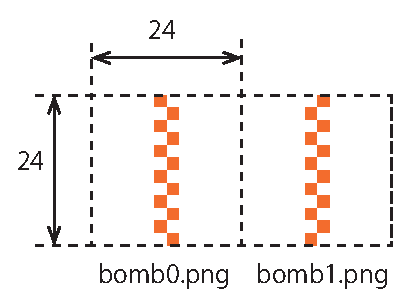
\includegraphics[width=0.3\hsize]{figures/eps/bomb0.eps}
  %\includegraphics[width=0.1\hsize]{bomb1.png}
\end{center}

bomb0.pngとbomb1.pngを交互に表示して動きを表現します

爆弾は4個用意しており、それぞれの爆弾は時限装置であるタイマー(time)を保持しています

movey()メソッドの引数delyは爆弾のスピードです。
またmovey()が呼ばれる度にcounterをインクリメントしています

爆弾の初期位置を-50に設定(top=-50)し、
時限装置(timer)を5から220の範囲の整数で設定しておきます

5回movey()メソッドが呼ばれると、爆弾の位置は画面の中に入ってきます
(爆弾の上端top$>$0)

counterの値が、爆弾の持っている時限装置の値を超えたら、
爆弾を落とす役目を担うエイリアンのオブジェクトを乱数で選び、
エイリアンと爆弾の位置を合わせて(bomb.center=enemy.center)爆弾を
投下させています

爆弾が画面の外に出たら(topが画面の高さを超える値になったら)、
再び爆弾を初期位置を-50にセットし、時限装置(time)の現在の値に
乱数の値(50〜250)を加えて、新たな時限装置としています
(counterの値が時限装置の値を超えた時に爆弾が投下されます)

\begin{lstlisting}[caption=Class Bombs,label=p007]
from random import randint
from Images import Images

class Bomb( Images ):
    def __init__(self, surface):
        super().__init__(surface, 'bomb0', 'bomb1')
        #super().__init__(surface, 48, 72)
        self.top = -50
        self.left = 0
        self.width = self.height = 24
        self.time = randint(5, 220)

class Bombs( Bomb ):
    def __init__(self, surface):
        self.surface = surface
        self.bombs = []
        for _ in range(4):
            self.bombs.append( Bomb(surface) )
        self.counter = 0
        self.stopflag = False

    def movey(self, aliens, dely=10):
        self.counter += 1
        for bomb in self.bombs:
            if bomb.top > 0:
                if not self.stopflag:
                    bomb.move(0, dely)
            if bomb.top > self.surface.get_rect().height:
                bomb.time += randint(50, 250)
                bomb.top = -50
            if bomb.time < self.counter and bomb.top < 0:
                enemy = aliens.aliens[randint(0, len(aliens.aliens)-1)]
                bomb.center = enemy.center

    def draw(self):
        for bomb in self.bombs:
            bomb.draw()

    def stop(self):
        self.stopflag = True
\end{lstlisting}

\subsubsection{Gameクラスの書き換え}

Gameクラスのコンストラクタで、Bombsクラスのオブジェクトを生成しています

ゲームの繰り返しループの中で、bombsオブジェクトを移動させ、描画しています

Bombsクラスのオブジェクトを移動させる時に、aliensオブジェクトを引数で渡しているのは、
aliensの中から乱数で選んだどれかのalienを起点として、Bombsクラスのオブジェクトを動かし始める必要があるからです

\begin{lstlisting}[caption=Gameクラス(bombオブジェクトを追加),label=p001-3]
import sys
import pygame
from pygame.locals import QUIT, KEYDOWN, K_RIGHT, K_LEFT, K_SPACE
from Screen import Screen
from Ship import Ship
from Beam import Beam
from Aliens import Aliens
from Bombs import Bombs

class Game( Screen ):
    BLACK = (0, 0, 0)
    def __init__(self):
        pygame.init()
            ・
            変更なし
            ・
        self.ship = Ship( self.surface )
        self.beam = Beam( self.surface )
        self.aliens = Aliens( self.surface )
        # Bombsクラスのオブジェクト生成を追加
        self.bombs = Bombs( self.surface )

    def fine(self):
        ・
        変更なし
        ・
    def key_event(self, ship, beam):
        ・
        変更なし
        ・
    def start(self):
        self.gameover = False
        while True:
            self.key_event( self.ship, self.beam )
              ・
              変更なし
              ・
            self.aliens.movexy()
            self.aliens.draw()
            self.bombs.movey( self.aliens ) # 追加:bombオブジェクトを動かして
            self.bombs.draw()               # 追加:bombオブジェクトを描画
            #
            pygame.display.update()
            self.clock.tick(self.FPS)
\end{lstlisting}

【演習】ここまでのプログラムを実行してみよう
(爆弾が投下されることを確認しよう)

\subsection{メッセージのクラス:Message}

\begin{lstlisting}[caption=Class Messages,label=p008]
import pygame

class Mess:
    def __init__(self, surface, size=80, color=(255,255,0)):
        self.surface = surface
        self.SIZE = size
        self.COLOR = color
        self.font = pygame.font.Font(None, size)
        self.MESSAGE = 'Hello'
        self.XPOS = self.YPOS = 0

    def display(self, msg=''):
        if msg=='':
            msg = self.MESSAGE
        text = self.font.render(msg, True, self.COLOR)
        textpos = text.get_rect()
        textpos.centerx = self.XPOS
        textpos.centery = self.YPOS
        self.surface.blit(text, textpos)

class Message( Mess ):
    def __init__(self, surface, message, xpos, ypos, size=80, color=(0,0,0)):
        super().__init__(surface, size, color)
        self.MESSAGE = message
        self.XPOS = xpos
        self.YPOS = ypos
\end{lstlisting}

\subsubsection{Gameクラスの書き換え}

Messagesクラスのオブジェクトを、3つ生成しています

AlienとBeamの干渉をclashedメソッドでチェックし、干渉があった場合は、beamをscreenの外に移し、同時にaliensを再構成しています

alien.collidepoint(beam.center)は、alienのRectの内部に、beam.centerの点座標が入っているかどうかを、bool変数で返します

また、干渉のあったalienオブジェクトが持っている得点をpoint変数に加算し、messagesオブジェクトに渡して、得点を表示しています

goverメソッドでは、aliensを全て倒したか、shipにbombが当たってゲームオーバーするか、
あるいは、aliensがscreenの下端まで進行してしまってゲームオーバーになるかを調べています

ゲームオーバーになったら、aliensもbombsも動きを止めるようにしています

\begin{lstlisting}[caption=Gameクラス(messageオブジェクトを追加),label=p008]
import sys
import pygame
from pygame.locals import QUIT, KEYDOWN, K_RIGHT, K_LEFT, K_SPACE
from Aliens import Aliens
from Beam import Beam
from Bombs import Bombs
from Message import Message
from Screen import Screen
from Ship import Ship

class Game( Screen ):
    BLACK = (0, 0, 0)
    def __init__(self):
        pygame.init()
          ・
          変更なし
          ・
        self.aliens = Aliens( self.surface )
        self.bombs = Bombs( self.surface )
        # 以下、Messageクラスのオブジェクトを3つ生成して追加
        self.gameover = False
        xpos = self.WIDTH//2
        ypos = self.HEIGHT//2
        YELLOW = (255,255,0)
        self.msg_gover = Message( self.surface,\
                                  'Game Over!!', xpos, ypos, color=YELLOW )
        self.msg_clear = Message( self.surface,\
                                  'Clear!!', xpos, ypos, color=YELLOW)
        ypos = 20
        self.msg_point = Message( self.surface,\
                                  'Point'+'=0', xpos, ypos, size=30, color=YELLOW )
        self.point = 0

    def fine(self):
        ・
        変更なし
        ・
    def key_event(self, ship, beam):
        ・
        変更なし
        ・
    # ゲームオーバーを判定するメソッドを追加
    def gover(self, aliens, ship, bombs):
        if not aliens.aliens:     # alienがいなくなったら
            self.msg_clear.display()
            self.gameover = True
        if aliens.area.bottom > self.HEIGHT-50: # alienが下端に達したら
            self.msg_gover.display()
            self.gameover = True
        for bomb in bombs.bombs:
            if bomb.colliderect(ship):    # bombがshipに当たったら
                self.msg_gover.display()
                self.gameover = True

    # beamがalianに当たったかどうか判定し、aliensを再構成するメソッドを追加
    def clashed(self, aliens, beam):
        tmp = []
        for alien in aliens.aliens:
            if alien.collidepoint(beam.center):
                self.point += alien.point       # beamがalienに当たったら
                beam.top = -50
            else:
                tmp.append(alien)
        aliens.aliens = tmp

    def start(self):
        self.gameover = False
        while True:
            self.key_event( self.ship, self.beam )
              ・
              変更なし
              ・
            self.bombs.movey( self.aliens )
            self.bombs.draw()
            # 追加:beamとalienの干渉チェック
            self.clashed( self.aliens, self.beam )
            # 追加:ゲームオーバーの判定
            self.gover( self.aliens, self.ship, self.bombs )
            # 追加:ゲームオーバーなら動きを止める
            if self.gameover:
                self.aliens.stop()
                self.bombs.stop()
            # 追加:得点表示のメッセージオブジェクト
            self.msg_point.display('Point='+str(self.point))
            pygame.display.update()
            self.clock.tick(self.FPS)
\end{lstlisting}

【演習】インベーダ ゲームが流行った当時のゲームでは、あるとき不意にUFOが現れ、
画面の上を右から左へ、或いは左から右へと移動していきました。
新たにUFOのクラスを追加し、もしUFOを打ち落としたら大きなボーナス特点が
得られるようにしましょう。

【演習】UFOが爆弾を投下するようにしてみましょう

【演習】UFOがランダムに画面の途中で行き来するような動きにしてみましょう

\newpage

\section{画像データの作成、編集}

インベーダゲームで使われる画像データを、自分でデザインできるようにします

24x24ピクセルの画像データを想定し、
画像データの編集には、Pillowライブラリを使います

\begin{center}
  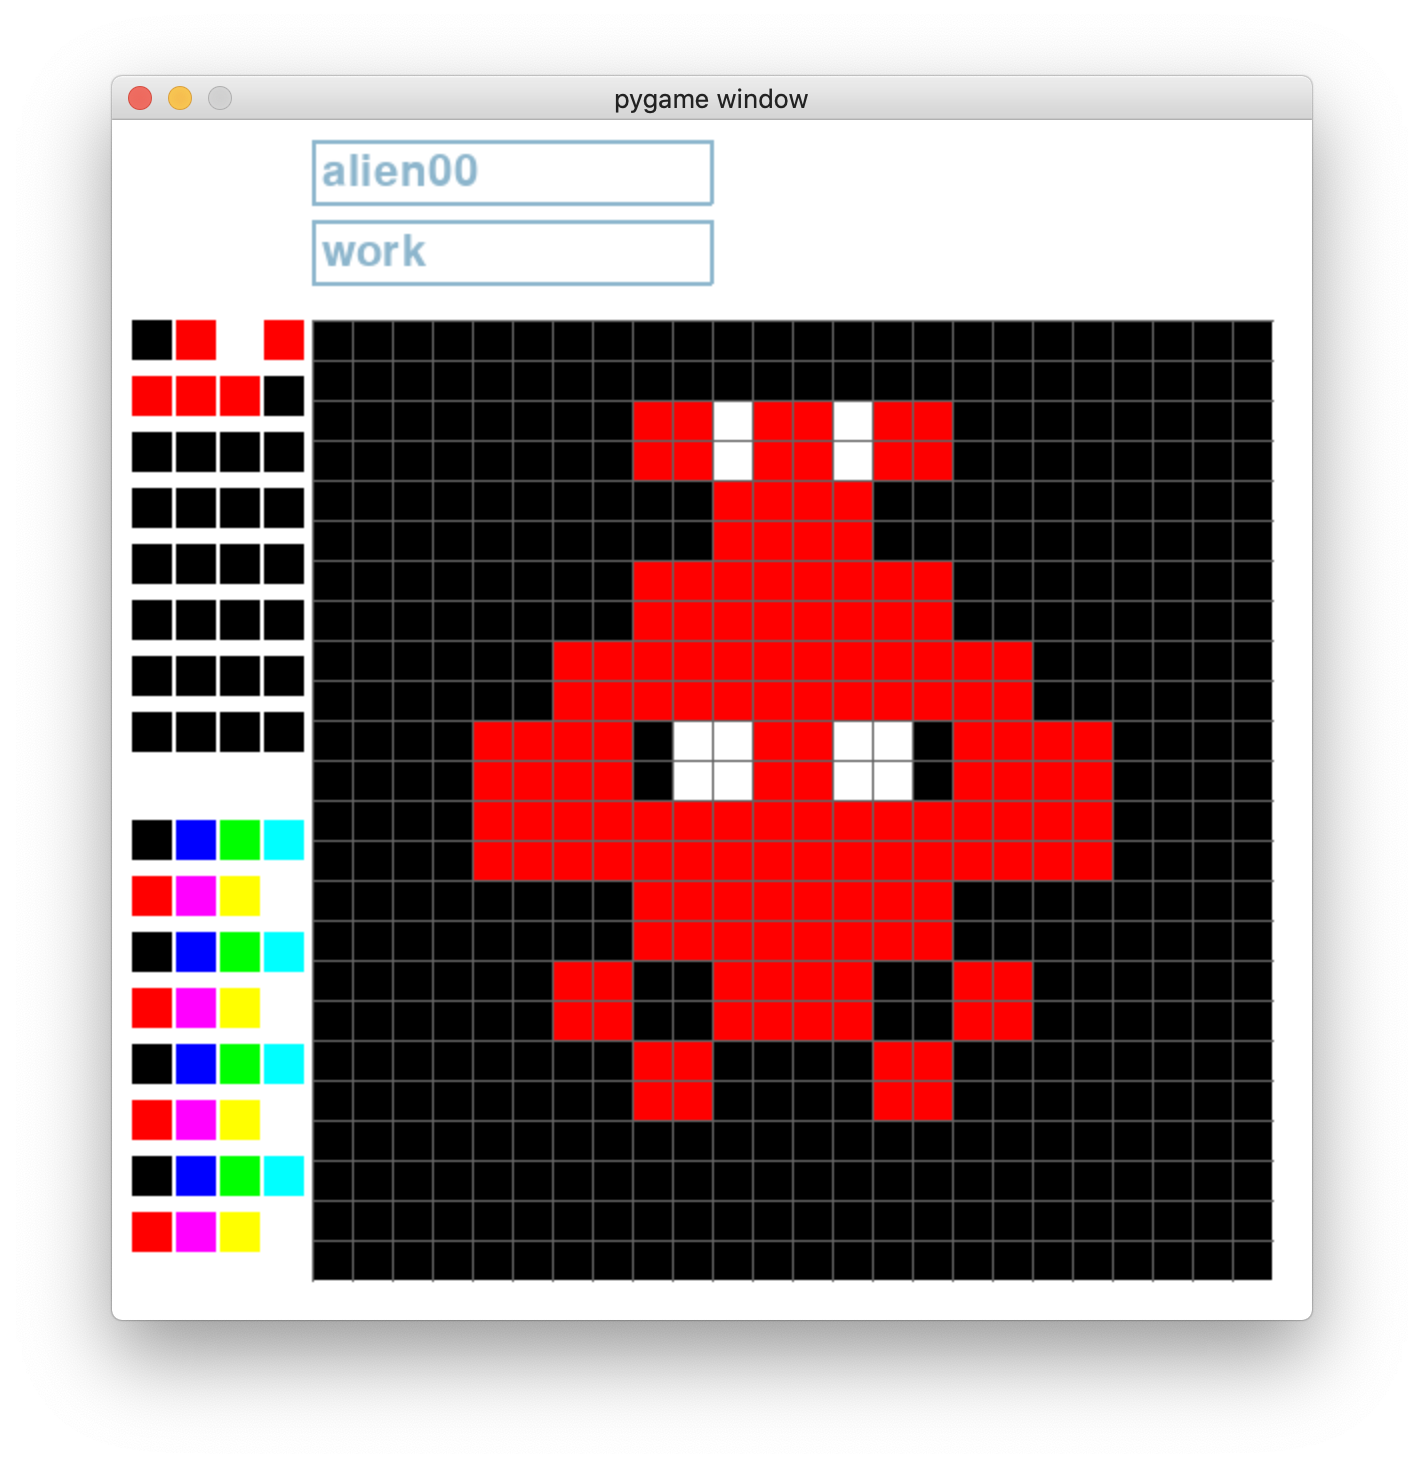
\includegraphics[width=0.75\hsize]{figures/eps/imageEdit.eps}
\end{center}

\subsection{画面管理のクラス:Screen}

作業画面の大きさと背景色を指定しています

キャプションを指定できるメソッド、画面を塗りつぶすメソッドを持っています

\begin{lstlisting}[caption=class Screen,label=pr03]
import pygame

class Screen:
    def __init__(self, size=(600,600), bgcolor=(0,0,0)):
        self.surface = pygame.display.set_mode(size)
        self.COLOR = bgcolor

    def fill(self):
        self.surface.fill(self.COLOR)

    def caption(self, str):
        pygame.display.set_caption(str)
\end{lstlisting}

\subsection{処理の流れを司るクラス:Editor}

main.pyは次のようにします

\begin{lstlisting}[caption=main.py,label=pr01]
from Editor import Editor

if __name__ == '__main__':
    ifname = 'invader200'
    ofname = 'work'
    edit = Editor(ifname, ofname)
    edit.start()
\end{lstlisting}

Editorクラスは、処理の主な流れを記述します

text0='alien00'は、編集したい入力画像のファイル名(alien00.png)を指定しています

text1='work'は、編集後の画像を保存するファイル名(work.png)を指定しています

Screenオブジェクトには、パレットが2つ、画像編集ボードが1つ、
元データファイル名と保存ファイル名のそれぞれの文字入力領域を配置しています

\begin{lstlisting}[caption=class Editor,label=pr02]
import sys
import pygame
from pygame.locals import QUIT, MOUSEBUTTONUP
from Board import Board
from Brush import Brush
from InputBox import InputBox
from Message import Message
from Palletes import Palletes
from Screen import Screen

class Editor:
    def __init__(self, ifname='alien00', ofname='work'):
        pygame.init()
        self.screen = Screen(bgcolor=(255,255,255))
        self.NUM = 24
        xoffset = 100
        yoffset = 100
        size = (600, 600)
        self.brush = Brush()
        self.board = Board(self.screen.surface, self.brush, xoffset, yoffset, self.NUM, (size[0], size[1]))
        self.text0 = text0 = ifname
        self.text1 = text1 = ofname
        self.board.pixels.load_image(text0)
        self.pallete1 = Palletes(self.screen.surface, self.brush, yoff=100, type=1)
        self.pallete2 = Palletes(self.screen.surface, self.brush, yoff=350, type=2)
        input_box1 = InputBox(100, 10, 140, 32, text0)
        input_box2 = InputBox(100, 50, 140, 32, text1)
        self.input_boxes = [input_box1, input_box2]
        self.message = Message()
        self.clock = pygame.time.Clock()
        self.FPS = 10

    def fine(self):
        if not self.input_boxes[1].text:
            text1 = self.text1
        else:
            text1 = self.input_boxes[1].text
        self.board.pixels.save_image('./'+text1+'.png')
        pygame.quit()
        sys.exit()

    def key_event(self):
        for event in pygame.event.get():
            if event.type == QUIT:
                self.fine()
            elif event.type == MOUSEBUTTONUP:
                if not self.board.paint(event.pos):
                    if not self.pallete1.select(event.pos):
                        self.pallete2.select(event.pos)
            else:
                for box in self.input_boxes:
                    box.handle_event(event)

    def start(self):
        while True:
            self.key_event()
            self.screen.fill()
            self.board.draw()
            self.pallete1.draw()
            self.pallete2.draw()
            for box in self.input_boxes:
                box.update()
                box.draw(self.screen.surface)
            text0 = self.input_boxes[0].text
            if text0!=self.text0:
                self.text0=text0
                self.board.pixels.load_image(text0)
                self.pallete1 = Palletes(self.screen.surface, self.brush, yoff=100, type=1)
            cstr = '(r,g,b) = ('+str(self.brush.color[0])+', '+str(self.brush.color[1])+', '+str(self.brush.color[2])+')'
            self.message.display(self.screen.surface, cstr, (320, 55))
            pygame.display.update()
            self.clock.tick(self.FPS)
\end{lstlisting}

\subsection{筆のクラス:Brush}

ブラシの現在色は、self.colorに保持させます

パレットは、self.colors1とself.colors2の2つを持っており、
それぞれに32色を持たせられます

self.colors2には、自分の好きな色を登録しておけば
画像編集の際にその色で描画することができます

self.colors1には、読み込んだ画像が持っている色が登録されるようにしています

\begin{lstlisting}[caption=class Brush,label=pr04]
class Brush:
    def __init__(self):
        self.color = (0,0,0)
        self.colors1 = []
        self.colors2 = []
        for _ in range(32):
            self.colors1.append((0,0,0))
            self.colors2.append((0,0,0))
        self.colors2[1] = (0,0,255)
        self.colors2[2] = (0,255,0)
        self.colors2[3] = (255,0,0)
        self.colors2[4] = (0,255,255)
        self.colors2[5] = (255,255,0)
        self.colors2[6] = (255,0,255)
        self.colors2[7] = (255,255,255)
        self.colors2[8] = (255,165,0)
        self.colors2[9] = (242,242,0)
        self.colors2[10] = (0,128,0)
        self.colors2[11] = (128,0,128)
        self.colors2[12] = (0,0,250)
\end{lstlisting}

\subsection{画像データ描画編集用盤面クラス:Board}

Boardクラスは、24x24ピクセルの画像編集領域です

パレットで色を選んで、現在色をbrushオブジェクトのcolorプロパティに設定し、
そのブラシで、boardオブジェクトのピクセルを塗るようにします

\begin{lstlisting}[caption=class Board,label=pr05]
import pygame
from pygame.locals import Rect
from Pixels import Pixels

class Board( Rect ):
    def __init__(self, surface, brush, xoff, yoff, num, size=(600, 600)):
        self.surface = surface
        self.brush = brush
        self.width = size[0]-xoff
        self.height = size[1]-yoff
        self.top = yoff
        self.left = xoff
        self.NUM = num
        self.SLOTW = self.width//num
        self.SLOTH = self.height//num
        self.fname = 'work'
        self.pixels = Pixels(self, self.fname)

    def draw(self):
        self.pixels.draw()
        GRAY = (100, 100, 100)
        for i in range(self.NUM):
            yy = self.SLOTH * i + self.top
            startp = (self.left, yy)
            endp = (self.right-self.SLOTW, yy)
            pygame.draw.line(self.surface, GRAY, startp, endp)
            xx = self.SLOTW * i + self.left
            startp = (xx, self.top)
            endp = (xx, self.bottom - self.SLOTH)
            pygame.draw.line(self.surface, GRAY, startp, endp)

    def paint(self, pos=(-1,-1)):
        def get_slot(xy):
            x, y = xy[0], xy[1]
            for ypos in range(self.NUM):
                y0 = self.top + self.SLOTH * ypos
                y1 = self.top + self.SLOTH * (ypos + 1)
                for xpos in range(self.NUM):
                    x0 = self.left + self.SLOTW * xpos
                    x1 = self.left + self.SLOTW * (xpos + 1)
                    if y0 < y < y1 and x0 < x < x1:
                        return xpos, ypos, ypos * self.NUM + xpos
            return -1,-1,-1

        x, y, n = get_slot(pos)
        if 0 <= n < len(self.pixels.pixels):
            self.pixels.pixels[n].set_color(self.brush.color)
            self.pixels.img.putpixel((x, y), self.brush.color)
            return True
        return False
\end{lstlisting}

\subsection{画素管理のクラス:Pixels、Pixel}

24x24ピクセルの画像の画素を管理しています

また、パレットの色の管理にも使っています

元画像データを読み込んだときに、そこで使われている色を、
boardオブジェクトが持っているbrushオブジェクトのcolors1プロパティに設定しています

元画像の読み込みや編集後の画像の保存のためのメソッドを持っています

画像を保存する際に、黒(r=g=b=0)の画素のalphaチャネルは0(透過)に設定しています

\begin{lstlisting}[caption=class Pixels,label=pr06]
import pygame
from PIL import Image
from pygame.locals import Rect

class Pixel( Rect ):
    def __init__(self, surface, color, rect):
        self.surface = surface
        self.COLOR = color
        self.left = rect[0]
        self.top = rect[1]
        self.width = rect[2]
        self.height = rect[3]

    def set_color(self, color):
        self.COLOR = color

    def draw_pixel(self):
        pygame.draw.rect(self.surface, self.COLOR, self)

class Pixels:
    def __init__(self, board, fname='work'):
        self.size=(board.NUM, board.NUM)
        width = board.SLOTW
        height = board.SLOTH
        r = g = b = 255
        self.pixels = []
        for y in range(board.NUM):
            top = board.SLOTH * y + board.top
            for x in range(board.NUM):
                left = board.SLOTW * x + board.left
                px = Pixel(board.surface, (r,g,b,255), (left, top, width, height))
                self.pixels.append( px )
        self.board = board
        self.img = self.load_image(fname)

    def load_image(self, fname):
        # 元画像の読み込み
        try:
            im = Image.open("./"+fname+".png")
            if im.size!=self.size:
                img = im.resize(self.size)
            else:
                img = im
        except Exception as f:
            print("Error with icon file:", f)
            img = Image.new('RGBA', self.size)
        self.img = img
        self.colors=[]
        for y in range(self.img.size[1]):
            for x in range(self.img.size[0]):
                col = self.img.getpixel((x, y))
                if col in self.colors:
                    pass
                else:
                    self.colors.append(col)
                pix = self.pixels[ y*self.board.NUM+x ]
                pix.set_color( col )
        for n, col in enumerate(self.colors):
            if n>len(self.board.brush.colors1)-1:
                break
            else:
                self.board.brush.colors1[n] = col

    def save_image(self, fname):
        img2 = Image.new('RGBA', self.size)
        for y in range(self.img.size[1]):
            for x in range(self.img.size[0]):
                pix = self.pixels[y * self.img.size[1] + x]
                r,g,b= pix.COLOR[0], pix.COLOR[1], pix.COLOR[2]
                #if r==g==b==0:
                if r<101 and g<101 and b<101:
                    r=g=b=a=0
                    #a=0
                else:
                    a=255
                img2.putpixel((x,y), (r,g,b,a))
        img2.save(fname)

    def draw(self):
        for p in self.pixels:
            p.draw_pixel()
\end{lstlisting}

\subsection{パレットの管理クラス:Palletes、Pallete}

\begin{lstlisting}[caption=class Palletes,label=pr07]
import pygame
from pygame.locals import Rect

class Pallete( Rect ):
    def __init__(self, surface, color, rect):
        self.surface = surface
        self.COLOR = color
        self.left = rect[0]
        self.top = rect[1]
        self.width = rect[2]
        self.height = rect[3]

    def set_color(self, color):
        self.COLOR = color

    def draw_pallete(self):
        pygame.draw.rect(self.surface, self.COLOR, (self.left, self.top, self.width, self.height))

class Palletes:
    def __init__(self, surface, brush, xoff=10, yoff=100, numx=4, numy=8, size=(90, 230), type=1):
        self.surface = surface
        self.brush = brush
        self.width = size[0]
        self.height = size[1]
        self.top = yoff
        self.left = xoff
        self.NUMX = numx
        self.NUMY = numy
        self.SLOTW = self.width//numx
        self.SLOTH = self.height//numy
        self.palletes = []
        self.palletegen(type)

    def palletegen(self, type=1):
        width = height = 20
        for y in range(self.NUMY):
            top = self.SLOTH * y + self.top
            for x in range(self.NUMX):
                left = self.SLOTW * x + self.left
                if type==1:
                    cl = self.brush.colors1[y*self.NUMX+x]
                else:
                    cl = self.brush.colors2[y*self.NUMX+x]
                pallet = Pallete(self.surface, cl, (left, top, width, height))
                self.palletes.append(pallet)

    def draw(self):
        for p in self.palletes:
            p.draw_pallete()

    def select(self, pos=(-1,-1)):
        def get_slot(xy):
            x, y = xy[0], xy[1]
            for ypos in range(self.NUMY):
                y0 = self.top + self.SLOTH * ypos
                y1 = self.top + self.SLOTH * (ypos + 1)
                for xpos in range(self.NUMX):
                    x0 = self.left + self.SLOTW * xpos
                    x1 = self.left + self.SLOTW * (xpos + 1)
                    if y0 < y < y1 and x0 < x < x1:
                        return ypos * self.NUMX + xpos
            return -1
        n = get_slot(pos)
        if 0 <= n < self.NUMX*self.NUMY:
            self.brush.color = self.palletes[n].COLOR
            return True
        return False
\end{lstlisting}

%\newpage

\subsection{文字列入力のクラス:InputBox}

\begin{lstlisting}[caption=class InputBox,label=pr08]
import pygame

class InputBox:
    def __init__(self, x, y, w, h, text=''):
        self.COLOR_INACTIVE = pygame.Color('lightskyblue3')
        self.COLOR_ACTIVE = pygame.Color('dodgerblue2')
        self.FONT = pygame.font.Font(None, 32)
        self.rect = pygame.Rect(x, y, w, h)
        self.color = self.COLOR_INACTIVE
        self.text = text
        self.txt_surface = self.FONT.render(text, True, self.color)
        self.active = False

    def handle_event(self, event):
        if event.type == pygame.MOUSEBUTTONDOWN:
            # If the user clicked on the input_box rect.
            if self.rect.collidepoint(event.pos):
                # Toggle the active variable.
                self.active = not self.active
            else:
                self.active = False
            # Change the current color of the input box.
            self.color = self.COLOR_ACTIVE if self.active else self.COLOR_INACTIVE
        if event.type == pygame.KEYDOWN:
            if self.active:
                if event.key == pygame.K_RETURN:
                    print(self.text)
                    self.text = ''
                elif event.key == pygame.K_BACKSPACE:
                    self.text = self.text[:-1]
                else:
                    self.text += event.unicode
                # Re-render the text.
                self.txt_surface = self.FONT.render(self.text, True, self.color)

    def update(self):
        # Resize the box if the text is too long.
        width = max(200, self.txt_surface.get_width()+10)
        self.rect.w = width

    def draw(self, screen):
        # Blit the text.
        screen.blit(self.txt_surface, (self.rect.x+5, self.rect.y+5))
        # Blit the rect.
        pygame.draw.rect(screen, self.color, self.rect, 2)
\end{lstlisting}

\subsection{文字列表示のクラス:Message}

\begin{lstlisting}[caption=class Message,label=pr09]
import pygame

class Message:
    def __init__(self, size=32, color=pygame.Color('dodgerblue2')):
        self.font = pygame.font.Font(None, size)
        self.color = color

    def display(self, surface, mess, locate):
        m = self.font.render(mess, True, self.color)
        surface.blit(m, locate)
\end{lstlisting}

\chapter{数独}

ここでのプログラムは短い簡易なものなので、オブジェクト指向で記述していません

再帰呼び出しについて学習する一つの例として、数独を解くプログラムを考えます

まず、boardリストに盤面を定義し、盤面の印刷を行う関数print\_board()を定義します

print\_board()をそのまま呼び出して、動作を確認してみましょう

\begin{lstlisting}[caption=board,label=sudoku01]
board = [[5,3,0,0,7,0,0,0,0],\
         [6,0,0,1,9,5,0,0,0],\
         [0,9,8,0,0,0,0,6,0],\
         [8,0,0,0,6,0,0,0,3],\
         [4,0,0,8,0,3,0,0,1],\
         [7,0,0,0,2,0,0,0,6],\
         [0,6,0,0,0,0,2,8,0],\
         [0,0,0,4,1,9,0,0,5],\
         [0,0,0,0,8,0,0,7,9]]

def print_board():
    global board
    for y in range(9):
        for x in range(9):
            print(' ',end='')
            if x in [2,5]:
                print(board[y][x], end=' |')
            else:
                print(board[y][x], end=' ')
        if y in [2,5]:
            print('\n---------|---------|--------')
        else:
            print()

# 動作確認
print_board()
\end{lstlisting}

\begin{verbatim}
  5  3  0 | 0  7  0 | 0  0  0
  6  0  0 | 1  9  5 | 0  0  0
  0  9  8 | 0  0  0 | 0  6  0
 ---------|---------|--------
  8  0  0 | 0  6  0 | 0  0  3
  4  0  0 | 8  0  3 | 0  0  1
  7  0  0 | 0  2  0 | 0  0  6
 ---------|---------|--------
  0  6  0 | 0  0  0 | 2  8  0
  0  0  0 | 4  1  9 | 0  0  5
  0  0  0 | 0  8  0 | 0  7  9
\end{verbatim}

次に、引数yとxで指定されたスロットに、
第三引数で受け取ったnを置く事ができるか否かを判定する関数possible()を定義します

(1) 縦一列の中に、nと同じ数字があったら置けませんので、Falseを返します

(2) 横一行の中に、nと同じ数字があったら置けませんので、Falseを返します

(3) 3$\times$3の枠の中に、nと同じ数字があったら置けませんので、Falseを返します

上記(1)、(2)、(3)の何れでもないなら、Trueを返します

5行5列目(boardリストの0行目や0列目から数え始めるので、引数はx=y=4)の空きスロットに値を指定して、possible()の動作を確認しましょう

\begin{lstlisting}[caption=possible,label=sudoku02]
def possible(y,x,n):
    global board
    for i in range(0,9):
        if board[y][i] == n:
            return False
    for i in range(0,9):
        if board[i][x] == n:
            return False
    x0 = (x//3)*3
    y0 = (y//3)*3
    for i in range(0,3):
        for j in range(0,3):
            if board[y0+i][x0+j] == n:
                return False
    return True

# 動作確認
print( possible(4,4,4) )
print( possible(4,4,5) )
\end{lstlisting}

最後に、問題を解く関数solve()を定義します

y行x列目のスロットに着目して、そこが0ならば空きスロットですから、
そのスロットに、1から10までの数字を順に指定して、possible()を呼びだしてはチェックしていきます

もし、possible()関数がTrueを返したら、それは一つの候補ですので、
引き続きsolve()を繰り返して空きスロットを埋めていきます

solve()がreturnでNoneを返したときは、選ばれた候補は使えなかったという事ですので、
盤面のスロットを空(0)に戻しています

全ての空欄が埋まったなら、print\_board()を呼んで結果(答え)を印刷しています

\begin{lstlisting}[caption=solve,label=sudoku03]
def solve():
    global board
    for y in range(9):
        for x in range(9):
            if board[y][x] == 0:
                for n in range(1,10):
                    if possible(y,x,n):
                        board[y][x] = n
                        solve()
                        board[y][x] = 0
                return
    print_board()

# 動作確認
solve()
\end{lstlisting}

solve()関数の中から、自分自身であるsolve()関数を呼び出す方法を再帰呼び出しと言います。
再帰呼び出しを使うことによって、プログラムを短く記述できています

実行結果

\begin{verbatim}
  5  3  4 | 6  7  8 | 9  1  2
  6  7  2 | 1  9  5 | 3  4  8
  1  9  8 | 3  4  2 | 5  6  7
 ---------|---------|--------
  8  5  9 | 7  6  1 | 4  2  3
  4  2  6 | 8  5  3 | 7  9  1
  7  1  3 | 9  2  4 | 8  5  6
 ---------|---------|--------
  9  6  1 | 5  3  7 | 2  8  4
  2  8  7 | 4  1  9 | 6  3  5
  3  4  5 | 2  8  6 | 1  7  9
\end{verbatim}

プログラムで解けてしまうとなると、しかも「こんなに短いプログラムで」解いたとなると、
数独そのものはつまらないものになりますね。
また「1から9まで総当たりで試しながら」=「コンピュータが力ずくで」なので、芸がないという気がします

このゲームは、まずは鉛筆と消しゴムを使って、自分で解いてみることが楽しむための重要なポイントのようです

【演習】

\begin{comment}

\chapter{ルービックキューブ}

\section{キューブの状態と操作手順の表現}

\subsection{表現方法(1)}

\begin{center}
  \includegraphics[width=0.8\hsize]{rubik.eps}
\end{center}

\newpage

U:上面をCWに90度 →
$\{37,39,45,43\},\{38,42,44,40\},\{03,27,16,28\},\{06,26,13,29\},\{09,25,10,30\}$

\begin{center}
  \includegraphics[width=0.65\hsize]{rubiku.eps}
\end{center}

D:下面をCWに90度 →
$\{46,48,54,52\},\{47,51,53,49\},\{12,19,07,36\},\{15,20,04,35\},\{18,21,01,34\}$

\begin{center}
  \includegraphics[width=0.65\hsize]{rubikd.eps}
\end{center}

\newpage

R:右面をCWに90度 →
$\{10,12,18,16\},\{11,15,17,13\},\{39,21,52,30\},\{42,24,49,33\},\{45,27,46,36\}$

\begin{center}
  \includegraphics[width=0.65\hsize]{rubikr.eps}
\end{center}

L:左面をCWに90度 →
$\{01,03,09,07\},\{02,06,08,04\},\{48,25,43,34\},\{51,26,40,31\},\{54,27,37,28\}$

\begin{center}
  \includegraphics[width=0.65\hsize]{rubikl.eps}
\end{center}

\newpage

F:前面をCWに90度 →
$\{28,30,36,34\},\{29,33,35,31\},\{09,45,18,54\},\{08,44,17,53\},\{07,43,16,52\}$

\begin{center}
  \includegraphics[width=0.65\hsize]{rubikf.eps}
\end{center}

B:後面をCWに90度 →
$\{19,21,27,25\},\{20,24,26,22\},\{01,46,10,37\},\{02,47,11,38\},\{03,48,12,39\}$

\begin{center}
  \includegraphics[width=0.65\hsize]{rubikb.eps}
\end{center}


\subsection{表現方法(2)}

\url{https://qiita.com/7y2n/items/a840e44dba77b1859352}

\begin{center}
  \includegraphics[width=0.8\hsize]{rubikalt.eps}
\end{center}

\begin{verbatim}
      |ーー センターパーツ:各面の中心のパーツ。1色で動かない。全部で6個。
パーツ ーー|ーー コーナーパーツ:キューブの角のパーツ。3色で動く。全部で8個。
      |ーー エッジパーツ :各辺の真ん中のパーツ。2色で動く。全部で12個。
\end{verbatim}

例えば、位置とパーツを次のように表現する

・ 位置0番にあるコーナーパーツ : 左上後の、白、橙、青、のパーツ

・ 位置2番にあるエッジパーツ : 右手前の、緑、赤、のパーツ

\subsection{状態を表すクラス:State}

ルービックキューブの状態を表すクラス State を定義する

\begin{lstlisting}[caption=State,label=rubik01]
class State:
    def __init__(self, cp, co, ep, eo):
        self.cp = cp
        self.co = co
        self.ep = ep
        self.ec = eo
\end{lstlisting}

\subsubsection{cp:Corner Permutation}
コーナーパーツの場所の情報を表す8次元ベクトル

i番目の要素(数値)は、現在コーナー位置i番にあるパーツの番号を表している

(例)cp = [1,2,0,3,4,5,6,7]

コーナー位置 0 番(左上後)には、1 番のコーナーパーツ(白青赤)が入っている

コーナー位置 1 番(右上後)には、2 番のコーナーパーツ(白赤緑)が入っている

などなど

\subsubsection{co:Corner Orientation}
コーナーパーツがどの向きを向いているかという情報を表す8次元ベクトル

各コーナーパーツは、以下の様に、3通りの向きをとることができる

U面D面色が、U面D面にあれば、0

時計方向に値切れていれば、1

反時計方向にねじれていれば、2

例えば、次の図の場合
\begin{center}
  \includegraphics[width=0.2\hsize]{cube1.eps}
\end{center}
位置1番にあるコーナーパーツは時計回りにねじれており、位置2番にあるコーナーパーツは反時計回りにねじれている

その他のパーツは全て白あるいは黄が上下に向いている

従って、co = [0,1,2,0,0,0,0,0]

\subsubsection{ep:Edge Permutation}
エッジパーツの場所の情報を保持している8次元ベクトル

\subsubsection{eo:Edge Orientation}
エッジパーツがどの向きを向いているかを表す12次元ベクトル

展開図で数字の書かれている色が、数字の書かれている面にあれば、0 とし、反転していたら、1 とします

展開図において、上U面(白)と下D面(黄)にある8つのエッジパーツ、前F面(緑)と後B面(青)にある4つのエッジパーツが基準面になります

【例】例えば、次の図の場合、
\begin{center}
  \includegraphics[width=0.2\hsize]{cube2.eps}
\end{center}
位置2番にあるエッジパーツは(一見反転しているように見えますが)、
現在その位置2番にいるパーツは、元は位置10番にあったエッジパーツであり、
位置10番のエッジパーツの基準面は黄色、
位置2番のエッジパーツの基準面は緑色であり、
基準面が基準面に収まっているという意味で、eoは0となります

この図の状態は、eo = [0,0,0,0,0,1,1,0,0,0,0,0]です

【例】完成状態の表現
\begin{center}
  \includegraphics[width=0.2\hsize]{cube3.eps}
\end{center}
コーナーパーツ:位置0番に0番のパーツがあって向きは0、…………、位置7番に7番のパーツがあって向きは0

エッジパーツ:位置0番に0番のパーツがあって向きは0、…………、位置11番に11番のパーツがあって向きは0、

完成状態は次のように表せる
\begin{lstlisting}[caption=solved State,label=rubik02]
solved_state = State(
    [0,1,2,3,4,5,6,7],
    [0,0,0,0,0,0,0,0],
    [0,1,2,3,4,5,6,7,8,9,10,11],
    [0,0,0,0,0,0,0,0,0,0, 0, 0]
)
\end{lstlisting}

【例】完成状態からRだけ操作した後の状態
\begin{center}
  \includegraphics[width=0.2\hsize]{cube4.eps}
\end{center}

\begin{lstlisting}[caption=r_state,label=rubik03]
r_state = State(
    [0,2,6,3,4,1,5,7],
    [0,1,2,0,0,2,1,0],
    [0,5,9,3,4,2,6,7,8,1,10,11],
    [0,0,0,0,0,0,0,0,0,0, 0, 0]
)
\end{lstlisting}

\subsection{操作を表すクラス}
操作を表すクラスは、新たに用意する必要はありません

操作は、状態を表すStateクラスでも表現できるからです

完成状態のsolved\_stateから操作Rを施した結果、
r\_stateが新たに得られたのですが、r\_stateはR操作そのものを
表しているともいえるからです

\subsection{操作するメソッド}

状態に対して操作を適用して、新たな状態を返すメソッドを追加します

引数で受け取っているmoveが操作をを表すStateクラスのインスタンスです

\begin{lstlisting}[caption=State,label=rubik04]
class State:
    def __init__(self, cp, co, ep, eo):
        self.cp = cp
        self.co = co
        self.ep = ep
        self.eo = eo

    def apply_move(self, move):
        new_cp = [self.cp[p] for p in move.cp]
        new_co = [(self.co[p] + move.co[i]) % 3 for i, p in enumerate(move.cp)]
        new_ep = [self.ep[p] for p in move.ep]
        new_eo = [(self.eo[p] + move.eo[i]) % 2 for i, p in enumerate(move.ep)]
        return State(new_cp, new_co, new_ep, new_eo)
\end{lstlisting}

【例】状態r\_stateに対して、操作r\_stateを適用して、r2\_stateを得る

\begin{lstlisting}[caption=R2,label=rubik05]
r2_state = r_state.apply_move( r_state )
print(f"r2_state.cp = {r2_state.cp}")
print(f"r2_state.co = {r2_state.co}")
print(f"r2_state.ep = {r2_state.ep}")
print(f"r2_state.eo = {r2_state.eo}")
\end{lstlisting}

\begin{verbatim}
  r2_state.cp = [0, 6, 5, 3, 4, 2, 1, 7]
  r2_state.co = [0, 0, 0, 0, 0, 0, 0, 0]
  r2_state.ep = [0, 2, 1, 3, 4, 9, 6, 7, 8, 5, 10, 11]
  r2_state.eo = [0, 0, 0, 0, 0, 0, 0, 0, 0, 0, 0, 0]
\end{verbatim}

こうして得られた状態r2\_stateは、R2操作でもあることになります
\begin{center}
  \includegraphics[width=0.2\hsize]{cube5.eps}
\end{center}

\subsubsection{cp(ep)の操作}

\begin{verbatim}
  new_cp = [self.cp[p] for p in move.cp]
  new_ep = [self.ep[p] for p in move.ep]
\end{verbatim}

具体例として、引数で受け取った$move.cp=[0,2,6,3,4,1,5,7]$を考えると、
もともとがr\_stateであったのですから、$self.cp$も$move\_cp$と同じ$self.cp=[0,2,6,3,4,1,5,7]$です

$move\_cp$を操作として考えれば、

新しい0番目の位置には、今0番の位置にあるパーツ(この例では0)が入ります

新しい1番目の位置には、今2番の位置にあるパーツ(この例では6)が入ります

新しい2番目の位置には、今6番の位置にあるパーツ(この例では5)が入ります
  などなど

結果としてできあがる新しいcpは、$[0, 6, 5, 3, 4, 2, 1, 7]$になります

\subsubsection{co(eo)の操作}

\begin{verbatim}
  new_co = [(self.co[p] + move.co[i]) % 3 for i, p in enumerate(move.cp)]
  new eo = [(self.eo[p] + move.eo[i]) % 2 for i, p in enumerate(move.ep)]
\end{verbatim}

具体例として、引数で受け取った$move.co=[0,1,2,0,0,2,1,0]$を考えると、
もともとがr\_stateであったのですから、$self.co$も$move\_co$と同じ$self.co=[0,1,2,0,0,2,1,0]$です

また$move\_cp$は、$move.cp=[0,2,6,3,4,1,5,7]$でした

coの場合は、操作によってコーナーパーツも移動してしまうので、それも加味する必要があります

$[self.co[p] for p in move.cp]$とすると、$[0,2,1,0,0,1,2,0]$が得られます

これはcpを加味して、次のような意味になります

新しく0番の位置に来るパーツ(今の0番の位置)のcoは0

新しく1番の位置に来るパーツ(今の2番の位置)のcoは2
  などなど

これで、新しくi番目の位置に来るパーツのもともとのねじれを取得したことになります

そして、それが更に$move.co$の各要素で指定された分ねじれることになるので、

new\_co = [self.co[p] + move.co[i] for i, p in enumerate(move.cp)]

とすることによって、$[0,3,3,0,0,3,3,0]$が得られることになります 

コーナーを3回ねじると、元のねじれに戻るので、各要素を3で割った余りを取って$[0,0,0,0,0,0,0,0]$になります

実際、白か黄色が上を向いているのが0なので、R2によってcoは全部0に戻ります

\subsection{全ての操作の定義}

操作の名前(RやR2)をkeyとして、その操作に対応するStateクラスのインスタンスを取得できるようにするためのdictを作ります

全部で18種類あります

\begin{lstlisting}[caption=moves,label=rubik06]
moves = {
    'U': State([3, 0, 1, 2, 4, 5, 6, 7],
               [0, 0, 0, 0, 0, 0, 0, 0],
               [0, 1, 2, 3, 7, 4, 5, 6, 8, 9, 10, 11],
               [0, 0, 0, 0, 0, 0, 0, 0, 0, 0, 0, 0]),
    'D': State([0, 1, 2, 3, 5, 6, 7, 4],
               [0, 0, 0, 0, 0, 0, 0, 0],
               [0, 1, 2, 3, 4, 5, 6, 7, 9, 10, 11, 8],
               [0, 0, 0, 0, 0, 0, 0, 0, 0, 0, 0, 0]),
    'L': State([4, 1, 2, 0, 7, 5, 6, 3],
               [2, 0, 0, 1, 1, 0, 0, 2],
               [11, 1, 2, 7, 4, 5, 6, 0, 8, 9, 10, 3],
               [0, 0, 0, 0, 0, 0, 0, 0, 0, 0, 0, 0]),
    'R': State([0, 2, 6, 3, 4, 1, 5, 7],
               [0, 1, 2, 0, 0, 2, 1, 0],
               [0, 5, 9, 3, 4, 2, 6, 7, 8, 1, 10, 11],
               [0, 0, 0, 0, 0, 0, 0, 0, 0, 0, 0, 0]),
    'F': State([0, 1, 3, 7, 4, 5, 2, 6],
               [0, 0, 1, 2, 0, 0, 2, 1],
               [0, 1, 6, 10, 4, 5, 3, 7, 8, 9, 2, 11],
               [0, 0, 1, 1, 0, 0, 1, 0, 0, 0, 1, 0]),
    'B': State([1, 5, 2, 3, 0, 4, 6, 7],
               [1, 2, 0, 0, 2, 1, 0, 0],
               [4, 8, 2, 3, 1, 5, 6, 7, 0, 9, 10, 11],
               [1, 1, 0, 0, 1, 0, 0, 0, 1, 0, 0, 0])
}
move_names = []
faces = list( moves.keys() )
for face_name in faces:
    move_names += [face_name, face_name + '2', face_name + '\'']
    moves[face_name + '2']  = moves[face_name].apply_move(moves[face_name])
    moves[face_name + '\''] = moves[face_name].apply_move(moves[face_name])\
                                              .apply_move(moves[face_name])
print(move_names)
\end{lstlisting}

\begin{verbatim}
['U','U2',"U'",'D','D2',"D'",'L','L2',"L'",'R','R2',"R'",'F','F2',"F'",'B','B2',"B'"]
\end{verbatim}

R2操作はR操作を2回適用して作っています

\'R操作はR操作を3回適用して作っています

\subsection{スクランブルState}

各操作記号を使ってスクランブル状態のインスタンスを作る

【例】
\begin{verbatim}
L D2 R U2 L F2 U2 L F2 R2 B2 R U' R' U2 F2 R' D B' F2
\end{verbatim}

この操作を施すと、次の状態が得られます

\begin{center}
  \includegraphics[width=0.2\hsize]{cube6.eps}
\end{center}

\begin{lstlisting}[caption=moves,label=rubik06]
# 完成状態
solved_state = State(
    [0,1,2,3,4,5,6,7],
    [0,0,0,0,0,0,0,0],
    [0,1,2,3,4,5,6,7,8,9,10,11],
    [0,0,0,0,0,0,0,0,0,0, 0, 0]
)
# スクランブル操作の文字列を適用した状態を得る関数
def scrambled_state(scramble):
    scrambled = solved_state
    for move_name in scramble.split(" "):
        move_state = moves[move_name]
        scrambled = scrambled.apply_move(move_state)
    return scrambled

# スクランブル操作
operate = "L D2 R U2 L F2 U2 L F2 R2 B2 R U' R' U2 F2 R' D B' F2"

# スクランブル操作を行う
scrambled = scrambled_state( operate )

# 確認する
print(f"scrambled state's cp = {scrambled.cp}")
print(f"scrambled state's co = {scrambled.co}")
print(f"scrambled state's ep = {scrambled.ep}")
print(f"scrambled state's eo = {scrambled.eo}")
\end{lstlisting}

\begin{verbatim}
  scrambled state's cp = [4, 3, 2, 1, 6, 5, 7, 0]
  scrambled state's co = [0, 0, 1, 0, 2, 2, 2, 2]
  scrambled state's ep = [2, 9, 4, 10, 0, 7, 3, 1, 11, 5, 6, 8]
  scrambled state's eo = [1, 1, 0, 0, 1, 0, 0, 0, 1, 0, 0, 0]
\end{verbatim}

\section{総当たりで解く}

「総当たり」で解くことをプログラムしていきます
(後半で「枝刈り」による高速化を試みます)

\subsection{完成状態か否かの判定}

\begin{lstlisting}[caption=is_solved,label=rubik07]
def is_solved(state):
    return state.eo == [0]*12 and state.co == [0]*8 and state.ep == list(range(12)) and state.cp == list(range(8))
\end{lstlisting}

\subsection{無駄な操作を判定}

\begin{lstlisting}[caption=is_move_available,label=rubik08]
inv_face = {"U":"D", "D":"U", "L":"R", "R":"L", "F":"B", "B":"F"}
def is_move_available(prev_move, move):
    """
    前の一手をもとに、次の一手として意味のある操作か否かを判定する
    ・同じ面を連続して操作しない(e.g. R'とR2など)
    ・対面を操作する時は順序を固定する(e.g. D Uは良しとし、U Dは不可とする など)
    """
    if prev_move is None:
        return True     # 最初の一手はあらゆる操作が可能
    prev_face = prev_move[0]    # 一手前で操作した面
    if prev_face == move[0]:
        return False            # 同一面の連続操作は不可
    if inv_face[prev_face] == move[0]:
        return prev_face < move[0]    # 対面操作の場合、辞書順なら可
    return True
\end{lstlisting}

\subsection{反復深化深さ優先探索}

\url{https://qiita.com/7y2n/items/24785b985e9c30862014}

\begin{lstlisting}[caption=Search class,label=rubik09]
class Search:
    def __init__(self):
        self.current_solution = []  # 今探索している手順を入れておくスタック

    def depth_limited_search(self, state, depth):
        if depth == 0 and is_solved(state):
            # is_solvedがTrueなら完成しているので解が見つかったということでTrueを返す
            # depth==0はなくてもいいが、depth > 0には解がないことがすでにわかっているのでいちいち判定関数を呼ぶ必要はない
            return True
        if depth == 0:  # depth 0 までたどり着いたのに解が見つからなかったらFalseを返す
            return False

        # depth=0まで探索を続ける
        prev_move = self.current_solution[-1] if self.current_solution else None  # 1手前の操作
        for move_name in move_names:
            if not is_move_available(prev_move, move_name):
                continue
            self.current_solution.append(move_name)
            if self.depth_limited_search(state.apply_move(moves[move_name]), depth - 1):
                return True
            self.current_solution.pop()

    def start_search(self, state, max_length=20):
        for depth in range(0, max_length):  # 0から次第に手数を増やしながら深さ制限探索を繰り返す
            print(f"# Start searching length {depth}")
            if self.depth_limited_search(state, depth):
                # 解が見つかったらその時点でそれを返却
                return " ".join(self.current_solution)
        return None
\end{lstlisting}

【例】

\begin{lstlisting}[caption=example,label=rubik10]
import time
# ルービックキューブの状態を表すクラス
class State:
    def __init__(self, cp, co, ep, eo):
        self.cp = cp
        self.co = co
        self.ep = ep
        self.eo = eo

    def apply_move(self, move):
        new_cp = [self.cp[p] for p in move.cp]
        new_co = [(self.co[p] + move.co[i]) % 3 for i, p in enumerate(move.cp)]
        new_ep = [self.ep[p] for p in move.ep]
        new_eo = [(self.eo[p] + move.eo[i]) % 2 for i, p in enumerate(move.ep)]
        return State(new_cp, new_co, new_ep, new_eo)
# 全ての操作を定義する
moves = {
    'U': State([3, 0, 1, 2, 4, 5, 6, 7],
               [0, 0, 0, 0, 0, 0, 0, 0],
               [0, 1, 2, 3, 7, 4, 5, 6, 8, 9, 10, 11],
               [0, 0, 0, 0, 0, 0, 0, 0, 0, 0, 0, 0]),
    'D': State([0, 1, 2, 3, 5, 6, 7, 4],
               [0, 0, 0, 0, 0, 0, 0, 0],
               [0, 1, 2, 3, 4, 5, 6, 7, 9, 10, 11, 8],
               [0, 0, 0, 0, 0, 0, 0, 0, 0, 0, 0, 0]),
    'L': State([4, 1, 2, 0, 7, 5, 6, 3],
               [2, 0, 0, 1, 1, 0, 0, 2],
               [11, 1, 2, 7, 4, 5, 6, 0, 8, 9, 10, 3],
               [0, 0, 0, 0, 0, 0, 0, 0, 0, 0, 0, 0]),
    'R': State([0, 2, 6, 3, 4, 1, 5, 7],
               [0, 1, 2, 0, 0, 2, 1, 0],
               [0, 5, 9, 3, 4, 2, 6, 7, 8, 1, 10, 11],
               [0, 0, 0, 0, 0, 0, 0, 0, 0, 0, 0, 0]),
    'F': State([0, 1, 3, 7, 4, 5, 2, 6],
               [0, 0, 1, 2, 0, 0, 2, 1],
               [0, 1, 6, 10, 4, 5, 3, 7, 8, 9, 2, 11],
               [0, 0, 1, 1, 0, 0, 1, 0, 0, 0, 1, 0]),
    'B': State([1, 5, 2, 3, 0, 4, 6, 7],
               [1, 2, 0, 0, 2, 1, 0, 0],
               [4, 8, 2, 3, 1, 5, 6, 7, 0, 9, 10, 11],
               [1, 1, 0, 0, 1, 0, 0, 0, 1, 0, 0, 0])
}
move_names = []
faces = list( moves.keys() )
for face_name in faces:
    move_names += [face_name, face_name + '2', face_name + '\'']
    moves[face_name + '2']  = moves[face_name].apply_move(moves[face_name])
    moves[face_name + '\''] = moves[face_name].apply_move(moves[face_name])\
                                              .apply_move(moves[face_name])
# 完成状態
solved_state = State(
    [0,1,2,3,4,5,6,7],
    [0,0,0,0,0,0,0,0],
    [0,1,2,3,4,5,6,7,8,9,10,11],
    [0,0,0,0,0,0,0,0,0,0, 0, 0]
)
# スクランブル操作の文字列を適用した状態を得る関数
def scrambled_state(scramble):
    scrambled = solved_state
    for move_name in scramble.split(" "):
        move_state = moves[move_name]
        scrambled = scrambled.apply_move(move_state)
    return scrambled
# 完成状態か否かを判定する
def is_solved(state):
    return state.eo == [0]*12 and state.co == [0]*8 and state.ep == list(range(12)) and state.cp == list(range(8))
# 無駄な操作を判別する
inv_face = {"U":"D", "D":"U", "L":"R", "R":"L", "F":"B", "B":"F"}
def is_move_available(prev_move, move):
    """
    前の一手をもとに、次の一手として意味のある操作か否かを判定する
    ・同じ面を連続して操作しない(e.g. R'とR2など)
    ・対面を操作する時は順序を固定する(e.g. D Uは良しとし、U Dは不可とする など)
    """
    if prev_move is None:
        return True     # 最初の一手はあらゆる操作が可能
    prev_face = prev_move[0]    # 一手前で操作した面
    if prev_face == move[0]:
        return False            # 同一面の連続操作は不可
    if inv_face[prev_face] == move[0]:
        return prev_face < move[0]    # 対面操作の場合、辞書順なら可
    return True
# 反復深化深さ優先探索
class Search:
    def __init__(self):
        self.current_solution = []  # 今探索している手順を入れておくスタック

    def depth_limited_search(self, state, depth):
        if depth == 0 and is_solved(state):
            # is_solvedがTrueなら完成しているので解が見つかったということでTrueを返す
            # depth==0はなくてもいいが、depth > 0には解がないことがすでにわかっているのでいちいち判定関数を呼ぶ必要はない
            return True
        if depth == 0:  # depth 0 までたどり着いたのに解が見つからなかったらFalseを返す
            return False

        # depth=0まで探索を続ける
        prev_move = self.current_solution[-1] if self.current_solution else None  # 1手前の操作
        for move_name in move_names:
            if not is_move_available(prev_move, move_name):
                continue
            self.current_solution.append(move_name)
            if self.depth_limited_search(state.apply_move(moves[move_name]), depth - 1):
                return True
            self.current_solution.pop()

    def start_search(self, state, max_length=20):
        for depth in range(0, max_length):  # 0から次第に手数を増やしながら深さ制限探索を繰り返す
            print(f"# Start searching length {depth}")
            if self.depth_limited_search(state, depth):
                # 解が見つかったらその時点でそれを返却
                return " ".join(self.current_solution)
        return None

if __name__=="__main__":
    operate = "R U R' F2 D2 L"
    scrambled = scrambled_state(operate)
    search = Search()
    start = time.time()
    solution = search.start_search( scrambled )
    print(f"Finished! ({time.time() - start:.2f} sec.)")
    if solution:
        print(f"Solution: {solution}.")
    else:
        print("Solution not found.")
\end{lstlisting}

実行結果

\begin{verbatim}
  # Start searching length 0
  # Start searching length 1
  # Start searching length 2
  # Start searching length 3
  # Start searching length 4
  # Start searching length 5
  # Start searching length 6
  Finished! (34.67 sec.)
  Solution: L' D2 F2 R U' R'.
\end{verbatim}

\subsection{枝刈りによる高速化}

もうこれ以上探索しても解に至らないと判断した場合、例えば、

depth=1(残り一手)の時点で、揃っているパーツが一つも無かったなら、
depth=0の探索を進めても無意味です
(完成状態から操作を一回行ってみると、
残りの一手の状態では、少なくともコーナー4個とエッジ8個が揃っていなければ、
次の一手で完成させることはできません)

depth=2(残り二手)の時点で、コーナーの全てが揃っていない可能性(L Rなど)がありますが、
エッジは必ず4つは揃っていないと、残り二手で完成させられる可能性はありません

depth=3(残り三手)では、その時点でエッジが少なくとも2個揃っていなければ、
残り三手で完成させることはできません

これらの知識を使った枝刈りを実装していきます

反復深化深さ優先探索を「知識あり」にしたものをIDA探索といいます

\url{https://en.wikipedia.org/wiki/Iterative_deepning_A}

\begin{lstlisting}[caption=IDA,label=rubik11]
#
# 揃っているコーナーの個数を数える
def count_solved_corners(state):
    return sum([state.cp[i]==i and state.co[i]==0 for i in range(8)])
# 揃っているエッジの個数を数える
def count_solved_edges(state):
    return sum([state.ep[i]==i and state.eo[i]==0 for i in range(12)])
# これ以上の探索が無意味ならTrueを返す関数
def prune(depth, state):
    # 残り一手で揃っているコーナーが4個未満、もしくは揃っているエッジが8個未満なら
    if depth==1 and (count_solved_corners(state) < 4 or count_solved_edges(state) < 8):
        return True
    # 残り二手で揃っているエッジが4個未満なら
    if depth==2 and count_solved_edges(state) < 4:
        return True
    # 残り三手で揃っているエッジが2個未満なら
    if depth==3 and count_solved_edges(state) < 2:
        return True
    return False
# Searchクラスの書き換え
class Search:
    def __init__(self):
        self.current_solution = []  # 今探索している手順を入れておくスタック

    def depth_limited_search(self, state, depth):
        if depth == 0 and is_solved(state):
            return True
        if depth == 0:
            return False
        # 枝刈り(次の2行を追加)
        if prune(depth, state):
            return False
        prev_move = self.current_solution[-1] if self.current_solution else None
        for move_name in move_names:
            if not is_move_available(prev_move, move_name):
                continue
            self.current_solution.append(move_name)
            if self.depth_limited_search(state.apply_move(moves[move_name]), depth - 1):
                return True
            self.current_solution.pop()

    def start_search(self, state, max_length=20):
        for depth in range(0, max_length):
            print(f"# Start searching length {depth}")
            if self.depth_limited_search(state, depth):
                return " ".join(self.current_solution)
        return None
\end{lstlisting}

先程と同じ例で実行してみます

\begin{lstlisting}[caption=example,label=rubik12]
#
if __name__=="__main__":
    operate = "R U R' F2 D2 L"
    scrambled = scrambled_state(operate)
    search = Search()
    start = time.time()
    solution = search.start_search( scrambled )
    print(f"Finished! ({time.time() - start:.2f} sec.)")
    if solution:
        print(f"Solution: {solution}.")
    else:
        print("Solution not found.")
\end{lstlisting}

\begin{verbatim}
  # Start searching length 0
  # Start searching length 1
  # Start searching length 2
  # Start searching length 3
  # Start searching length 4
  # Start searching length 5
  # Start searching length 6
  Finished! (0.28 sec.)
  Solution: L' D2 F2 R U' R'.
\end{verbatim}

34秒かかっていた探索が、1秒未満になりました

最初の解が見つかった段階ですぐにreturnせず、更に探索を続けるようにすれば、複数の解を探すこともできます

\section{Two-Phase-Algorithm}

\url{https://qiita.com/7y2n/items/55abb991a45ade2afa28}

現実的な時間でルービックキューブの準最適解を見つけるアルゴリズムとして、Two-Phase-Algorithmが広く使われている

ルービックキューブの解法を2つのPhaseに分解して、それぞれを総当たり(IDA探索)で解くという方法

Phase1では、自由に動かして、\<U, D, R2, L2, F2, B2\>の動きだけで完成できる状態に持っていきます(約10手、最悪でも12手程度)

Phase2では、\<U, D, R2, L2, F2, B2\>の動きだけを使って完成まで持っていきます(約13手〜14手で完成に至る)

Phase1のゴールは、\<U, D, R2, L2, F2, B2\>の動きだけで完成できる状態に持っていくこと

これは、完成状態から上面と下面は90度回して良いが、側面は180度しか回さないでたどり着ける状態まで絞り込むと言うこと

実際に完成状態から\<U, D, R2, L2, F2, B2\>の動きだけで崩してみると、
(その状態は、Phase1の到達状態なのですが)次のような特徴がある

\begin{itemize}
\item COが全て揃っている
\item EOが全て揃っている
\item U面とD面に挟まれた中層(以下E列と呼ぶ)のエッジパーツ(エッジパーツ0,1,2,3)はE列内でしか移動していない
\end{itemize}

逆に、この3つが満たされている状態は、Phase1の完成状態だということになる
(CPやE列以外のEPの状態は関係ない)

Phase1では、

\begin{itemize}
\item COには2187通り($3^7$)の状態がある
\item EOには2018通り($2^{11}$)の状態がある
\item E列のエッジパーツの配置には495通り($_{12} \mathrm{C} _4$)の状態がある
\end{itemize}

COは、ねじれの総和が3の倍数になることが分かっていて、7個決まれば残りの1つは決まるので3の7乗となる

EOは、11個決まれば残りの1つは決まるので、2の11乗となる

Phase2では、

Phase1での達成状態(COが揃っている、EOが揃っている、E列のパーツがE列内にある)は、Phase2の操作では崩れないことを担保するので、

\begin{itemize}
\item CPには40320通り($8!$)の状態がある
\item UD面の8つのエッジパーツのEPの状態には40320通り($8!$)の状態がある
\item E列の4つのエッジパーツEPの状態には24通り($4!$)の状態がある
\end{itemize}

\subsubsection{定数}

定数をクラス変数として用意します

\begin{lstlisting}[caption=Constant,label=rubik13]
class Constant:
    NCORNERS = 8
    NEDGES = 12
    NCO = 2187 # 3**7
    NEO = 2048 # 2 ** 11
    NE_COMBINATIONS = 495 # 12C4
    NCP = 40320 # 8!
    NEP = 479001600 # 12!
    NUDEP = 40320 # 8!
    NEEP = 24 # 4!
\end{lstlisting}

\subsection{状態のindex化}

\subsubsection{Phase1の状態のindex化}

【COのindex化】

【EOのindex化】

【E列のエッジパーツの位置の組み合わせのindex化】

\subsubsection{Phase2の状態のindex化}

【CPのindex化】

【UD面のEPのindex化】

【E列のEPのindex化】

\subsection{遷移表の構築}

\subsubsection{Phase1の遷移表}

【COの遷移表】

【EOの遷移表】

【E列エッジの組み合わせの遷移表】

\subsubsection{Phase2の遷移表}

【CPの遷移表】

【UD面エッジのEPの遷移表】

【E列エッジのEPの遷移表】

\subsection{枝刈り表の構築}

\subsubsection{Phase1の枝刈り表}

【EOを無視して、COとE列だけを考えたときの最短手順】

【COを無視して、EOとE列だけを考えたときの最短手順】

\subsubsection{Phase2の枝刈り表}

【UD面のエッジを無視して、CPとE列エッジだけ揃える時の最短手順表】

【CPを無視して、UD面のエッジとE列エッジだけ揃える時の最短手順】

\subsection{Phase1の探索}

\end{comment}

\chapter{三目並べ(Tic-Tac-Toe)}

三目並べは「二人零和有限確定完全情報ゲーム」と呼ばれるゲームに分類されます.
簡単に言うと「勝敗は偶然に左右されず,最善手を打てばどちらかが勝つまたは引き分けになるゲーム」のことです.
他にもリバーシ,チェッカー,チェス,将棋に囲碁などもこのゲームに分類されます.

初めに三目並べというゲームについて定義をしておきます.

三目並べ:
3×3の格子上に二人のプレイヤーが「O」「X」を配置し、自分のマークを先に3つ並べた方が勝ちです.

\section{CUI(Character User Interface)版}

\subsection{太郎さんと花子さんの対戦}

プログラムを実行すると盤面が表示され、×の石を置く場所を指定するよう促されます

画面上に示された番号を入力すると、その番号のスロットに×の石が置かれた盤面が表示され、次の手番の○に、石を置く場所を指定するように促されます

手番を交互に変えながらゲームは進み、縦、横、斜めの何れかに、先に一列に自分の石を並べた方が勝ちとなります

既に石の置かれているスロット番号を指定できませんし、スロット番号として 0 〜 8 以外の数値を指定することもできません

\begin{spacing}{0.74}
  \begin{verbatim}
    スタート! [Tic Tac Toe]
    /---|---|---\
    | 0 | 1 | 2 |
    |---|---|---|
    | 3 | 4 | 5 |
    |---|---|---|
    | 6 | 7 | 8 |
    \---|---|---/
    太郎 さんのturnです。スロット番号を指定して下さい : 4
    /---|---|---\
    | 0 | 1 | 2 |
    |---|---|---|
    | 3 | X | 5 |
    |---|---|---|
    | 6 | 7 | 8 |
    \---|---|---/
    花子 さんのturnです。スロット番号を指定して下さい : 2
    /---|---|---\
    | 0 | 1 | O |
    |---|---|---|
    | 3 | X | 5 |
    |---|---|---|
    | 6 | 7 | 8 |
    \---|---|---/
    太郎 さんのturnです。スロット番号を指定して下さい :
  \end{verbatim}
\end{spacing}

\subsubsection{ゲームの進行を司るクラス:Game}

Gameクラスのオブジェクトであるgameを生成し、
gameオブジェクトの中のstart()というメソッドを実行します

この後、main.pyとGame.pyでファイルを別にしていきますので、
以下のように、main.pyを書いて、
その冒頭で、Game.pyからGameというクラスをimportするという記述が必要になります

\begin{lstlisting}[caption=main.py,label=prog01-3-1]
from Game import Game

if __name__ == '__main__':
    game = Game()
    game.start()
\end{lstlisting}%

\subsubsection{盤面を管理するクラス:Board}

ゲームの盤面を保持するクラスBoardを作っていきます

Boardクラスのオブジェクトboardを、Gameクラスのコンストラクタで生成することにします

ゲームの進行を行うstart()メソッドでは、boardオブジェクトを印刷するメソッドdraw()を呼び出すようにしています

Gameクラスで、Boardクラスを使っていますから、
そのファイルの冒頭で、BoardファイルからBoardクラスをimportせよという指示が必要です

\begin{lstlisting}[caption=class Game,label=prog02-1]
from Board import Board

class Game:
    def __init__(self):
        self.board = Board()

    def start(self):
        self.board.draw()
\end{lstlisting}%

盤面の実体は、各スロットに対応させた9個の整数からなるリストboardで保持することとし、Boardクラスのコンストラクタで準備を整えます

draw()メソッドは、盤面boardの状態を画面に表示する処理を行っています

9個の文字からなるリストbdを用意して、boardの値が0なら空きスロット、
整数の1なら一人目のプレイヤーの石、整数の2なら二人目のプレイヤーの石が置かれている
として、それぞれ文字'X'と'O'の文字を表示させています

print()関数で、「文字列.format」という書き方によって、\{\}の位置にbdの文字を書いていますが、
「文字列.format」という書き方よりも、「f文字列」という書き方によって\{\}に値を埋め込む方が
Pythonicな書き方だと「Effective Python」の項目4には書かれています

\begin{lstlisting}[caption=class Board,label=prog02-2]
class Board:
    def __init__(self):
        self.board = [0,0,0,\
                      0,0,0,\
                      0,0,0]

    def draw(self):
        bd = ['', '', '',\
              '', '', '',\
              '', '', '']
        n = 0
        for val in self.board:
            if val==0:
                bd[n] = str(n)
            elif val==1:
                bd[n] = 'X'
            elif val==2:
                bd[n] = 'O'
            n += 1
        print( '/---|---|---\\')
        print( '| {} | {} | {} |'.format(bd[0], bd[1], bd[2]) )
        print( '|---|---|---|')
        print(f'| {bd[3]} | {bd[4]} | {bd[5]} |')
        print( '|---|---|---|')
        print(f'| {bd[6]} | {bd[7]} | {bd[8]} |')
        print( '\\---|---|---/')
\end{lstlisting}%

\subsubsection{プレーヤのクラス:Player}

Gameクラスのコンストラクタの中で、
Playerクラスのオブジェクトとして、taroとhanakoを生成しています。
Playerクラスのコンストラクタへの、
一つ目の引数で名前を、二つ目の引数で盤面におく石に対応づけた整数を渡しています。

この整数は、taroとhanakoの識別子としての役割を持たせますので、区別できる値でなければなりません。

また、gameオブジェクトの中でPLAYERというリストを定義して、
taroとhanakoというPlayerクラスのオブジェクトのリストを作っています。
PLAYER[0]によってtaroオブジェクトを、PLAYER[1]によってhanakoオブジェクトを
取り出せることになります。

ゲームの進行は大まかにいうと、①盤面を表示して、②一方のプレーヤを選んで、③そのプレーヤが盤面上に石を置いて、④手番を交代して、
をゲームオーバーまで繰り返すことになります

\begin{lstlisting}[caption=class Game,label=prog03-1]
from Board import board
from Player import Player

class Game:
    def __init__(self):
        self.board = Board()
        taro = Player('太郎', 1)
        hanako = Player('花子', 2)
        self.PLAYER = [taro, hanako]

    def start(self):
        turn = 0
        while True:                       # 以下をゲームオーバーまで繰り返す
            self.board.draw()                 # ①盤面を表示して
            player = self.PLAYER[ turn ]      # ②プレーヤを選んで
            player.put_stone( self.board )    # ③そのプレーヤが盤面に石を置いて
            turn = (turn+1) % 2               # ④手番を交代する
\end{lstlisting}%

Playerクラスでは、そのコンストラクタで、
引数で受け取った名前と番号を各オブジェクトに保存するようにしています

put\_stone()メソッドでは、input()文でプレーヤにスロット番号の入力を促し、
受け取った番号(文字列s)をint(文字列)関数によって整数に変換して、
盤面board上のスロット番号の位置に、このプレーヤオブジェクトが保持しているid番号(1か2)を納めています

\begin{lstlisting}[caption=class Player,label=prog03-2]
from Board import Board

class Player:
    def __init__(self, name, id):
        self.name = name
        self.id = id

    def put_stone(self, board):
        s = input(self.name + "さんの手番です。スロット番号は? : ")
        n = int(s)
        board.board[ n ] = self.id
\end{lstlisting}%

\subsubsection{勝敗の判定}

Boardクラスのwinner()メソッドでは、
行方向に3つ(row0, row1, row2)、列方向に3つ(col0, col1, col2)、斜め方向に2つ(crs0, crs1)のそれぞれで、
各スロットの中の値が一致しているか否かをチェックしています

行または列、斜めのどれか一つでも一致しているものがあったら、そのときのplayerの勝ちです

\begin{lstlisting}[caption=class Board,label=prog03-5]
class Board:
    def __init__(self):
        self.board = [0,0,0,0,0,0,0,0,0]

    def draw(self):
        bd = ['', '', '','', '', '','', '', '']
        for n, val in enumerate( self.board ):
            ・
            変更なし
            ・
        print( '\\---|---|---/')

    # 以下を追加
    def winner(self, player):
        row0 = self.board[0]!=0 and\
               self.board[0]==self.board[1] and self.board[0]==self.board[2]
        row1 = self.board[3]!=0 and\
               self.board[3]==self.board[4] and self.board[3]==self.board[5]
        row2 = self.board[6]!=0 and\
               self.board[6]==self.board[7] and self.board[6]==self.board[8]
        col0 = self.board[0]!=0 and\
               self.board[0]==self.board[3] and self.board[0]==self.board[6]
        col1 = self.board[1]!=0 and\
               self.board[1]==self.board[4] and self.board[1]==self.board[7]
        col2 = self.board[2]!=0 and\
               self.board[2]==self.board[5] and self.board[2]==self.board[8]
        crs0 = self.board[0]!=0 and\
               self.board[0]==self.board[4] and self.board[0]==self.board[8]
        crs1 = self.board[2]!=0 and\
               self.board[2]==self.board[4] and self.board[2]==self.board[6]
        if col0 or col1 or col2 or row0 or row1 or row2 or crs0 or crs1:
            return True
\end{lstlisting}%

勝敗を判定して結果を表示し、breakによってゲームのループを抜けます

\begin{lstlisting}[caption=class Game,label=prog03-6]
from Board import Board
from Player import Player

class Game:
    def __init__(self):
        self.board = Board()
        taro = Player('太郎', 1)
        hanako = Player('花子', 2)
        self.PLAYER = [taro, hanako]

    def start(self):
        turn = 0
        while True:
            self.board.draw()
            player = self.PLAYER[turn]

            b1 = self.board.winner()
            if b1:
                print( player.name + 'さん の勝ち')
                break

            turn = (turn+1) % 2
\end{lstlisting}%

\subsubsection{引き分けの判定}

%Playerクラスのput\_stone()の引数で、Boardクラスのオブジェクトboardを受け取っています。
boardオブジェクトが持っているboardプロパティは、9個の各スロットの状態(空かマルかバツか→0か1か2か)を保持するリストでした。
スロットが空き(スロットの値がゼロ)であれば、石を置くことができます。

値がゼロのスロット番号(n)を集めたリストをvacantに作り、その長さはlen()関数で調べることができます。
リストの長さがゼロであるということは、空のスロット(値がゼロのスロット)は無くなったということですから、もう石を置くことはできません(このとき引き分けです)。

\begin{figure}[H]
  \centering
  \begin{tabular}{ll}
      \begin{minipage}{0.5\hsize}
      \centering
      \begin{lstlisting}[caption=,label=prog03-03]
      # 引き分けの判定はここから
      empty = []
      n = 0
      for slot in board.board:
          if slot==0:
              empty.append( n )
          n += 1
      if len( empty )==0:
          return False
      # ここまで
      \end{lstlisting}%
      \end{minipage}
      \begin{minipage}{0.5\hsize}
      \flushright
      \begin{lstlisting}[caption=,label=prog03-04]
      # 引き分けの判定はここから
      empty = []
      for n in range( len(board.board) ):
          slot = board.board[n]
          if slot==0:
              empty.append( n )

      if len( empty )==0:
          return False
      # ここまで
      \end{lstlisting}%
      \end{minipage}
    \end{tabular}
\end{figure}%

引き分けの判定部分は、上のように書くこともできますが、ここでは
以下のようなenumerate()関数の使い方を学習しましょう。
「Effective Python」には項目7で、rangeではなくenumerateを使うのが
Pythonicだとされています。

また、if len( empty )==0: という記述は、if not empty: と書いた方がPythonicだと同じ本の第一章には書かれています。

\begin{lstlisting}[caption=class Board,label=prog03-5]
class Board:
    def __init__(self):
        self.board = [0,0,0,0,0,0,0,0,0]

    def draw(self):
        bd = ['', '', '','', '', '','', '', '']
        for n, val in enumerate( self.board ):
            ・
            変更なし
            ・
        print( '\\---|---|---/')

    def winner(self, player):
            ・
            変更なし
            ・
        if col0 or col1 or col2 or row0 or row1 or row2 or crs0 or crs1:
            return True

    # 以下を追加
    def vacant(self):
        empty = []
        for n, slot in enumerate(self.board):
            if slot == 0:
                empty.append(n)
        return empty
\end{lstlisting}%

入力されたスロット番号nが、vacantリストの中にあることを確認すること(if n in vacant:)によって、
既に置かれた石の上に上書きすることを防いでいます。

今の段階で、
put\_stone()メソッドが返す値は、Falseならば引き分け、Trueならばボード上に石を置きましたという意味になります

\begin{lstlisting}[caption=class Player,label=prog03-3]
from Board import Board

class Player:
    def __init__(self, name, id):
        self.name = name
        self.id = id

    def put_stone(self, board):
        # 引き分けの判定はここから
        vacant = board.vacant()
        if not vacant:
          return False
        # ここまで
        while True:
            s = input(self.name + "さんの手番です。スロット番号は? : ")
            n = int(s)
            if n in vacant:      # 空きスロットのリストに番号nは含まれているか?
                board.board[ n ] = self.id
                break
        return True
\end{lstlisting}%

Gameクラスでは、put\_stone()メソッドを呼び出して判定する必要があります

引き分けの判定(b2)でFalseが返された(not b2 == True)なら、'引き分け'と表示してゲームの反復を抜けます(break)

b2 が Trueを返してきた場合は、順当にその時の手番(turn)のplayerオブジェクトが、
盤面オブジェクト(self.board)に石を置いた(put\_stone()した)場合になりますから、そのままゲームを続行します

引き分けと勝敗の判定を、ゲーム進行の途中に入れています

引き分けた場合、あるいは勝敗のついた場合のいずれの場合でも、
break文によってゲームの進行(反復)を終えています

\begin{lstlisting}[caption=class Game,label=prog03-6]
from Board import Game
from Player import Player

class Game:
    def __init__(self):
        self.board = Board()
        taro = Player('太郎', 1)
        hanako = Player('花子', 2)
        self.PLAYER = [taro, hanako]

    def start(self):
        turn = 0
        while True:
            self.board.draw()
            player = self.PLAYER[turn]

            b2 = player.put_stone( self.board )
            if not b2:
                print('引き分け')
                break

            b1 = self.board.winner()
            if b1:
                print( player.name + 'さん の勝ち')
                break

            turn = (turn+1) % 2
\end{lstlisting}%

\subsection{太郎さんとコンピュータの対戦}

花子さんをコンピュータに変更します

Gameクラスの最初、コンストラクタでPlayerクラスのオブジェクト生成を変更します

\begin{lstlisting}[caption=class Game,label=prog04-1]
from Board import Game
from Player import Player

class Game:
    def __init__(self):
        self.board = Board()
        human = Player('Taro', 1)         # 変更点はここから3行
        machine = Player('computer', 2)
        self.PLAYER = [human, machine]

    def start(self):
        turn = 0
        while True:
            self.board.draw()
                ・
                ・   この部分に変更なし
                ・
\end{lstlisting}%

Playerクラスでは、
computer オブジェクトの場合には乱数によって、vacantリストの中から石をおくスロット番号を選ぶようにします

humanオブジェクトの場合は、スロット番号の入力を促しています

Playerクラスのオブジェクトは、humanの場合とmachineの場合がありますから、
Playerクラスのそれぞれのオブジェクトが持っているself.idの値を見て、
それが1ならhumanオブジェクト、2ならmachineオブジェクトだと判定している部分に注目しましょう

\begin{lstlisting}[caption=class Player,label=prog04-2]
from Board import Board

class Player:
    def __init__(self, name, id):
        self.name = name
        self.id = id

    def put_stone(self, board):
        # 引き分けの判定はここから
        vacant = board.vacant()
        if not vacant:
            return False
        # 変更点は以下の部分
        if self.id == 2:      # Computerの場合は乱数で
            n = randint( 0, len(vacant)-1 )
            board.board[ vacant[n] ] = self.id
        else:                 # Taroの場合はキーボード入力でスロット番号を指定させる
            while True:
                s = input(self.name + "さんの手番です。スロット番号は? : ")
                n = int(s)
                if n in vacant:
                    board.board[ n ] = self.id
                    break
        return True
\end{lstlisting}%

winner()メソッドをもう少し簡潔に記述し直すことにしましょう

\begin{lstlisting}[caption=class Board,label=prog04-3]
class Board:
          .
          . この部分に変更なし
          .
    def winner(self, player):
        def scan(n1, n2, n3):
            return self.board[n1]!=0 and\
                   self.board[n1]==self.board[n2] and\
                   self.board[n1]==self.board[n3]:
        return scan(0,1,2) or scan(3,4,5) or scan(6,7,8) or\
               scan(0,3,6) or scan(1,4,7) or scan(2,5,8) or\
               scan(0,4,8) or scan(2,4,6)
\end{lstlisting}%

\section{GUI(Graphical User Interface)版}

ここまではCUI(Character User Interface)ベースのゲームでしたが、
ここからは、Pygameを使ってGUI(Graphical User Interface)版のゲームを作っていきます

新しいプロジェクトを開始することにしましょう

まずは、コンピュータが乱数で石を置いてくる単純な方法を実現します

\begin{center}
  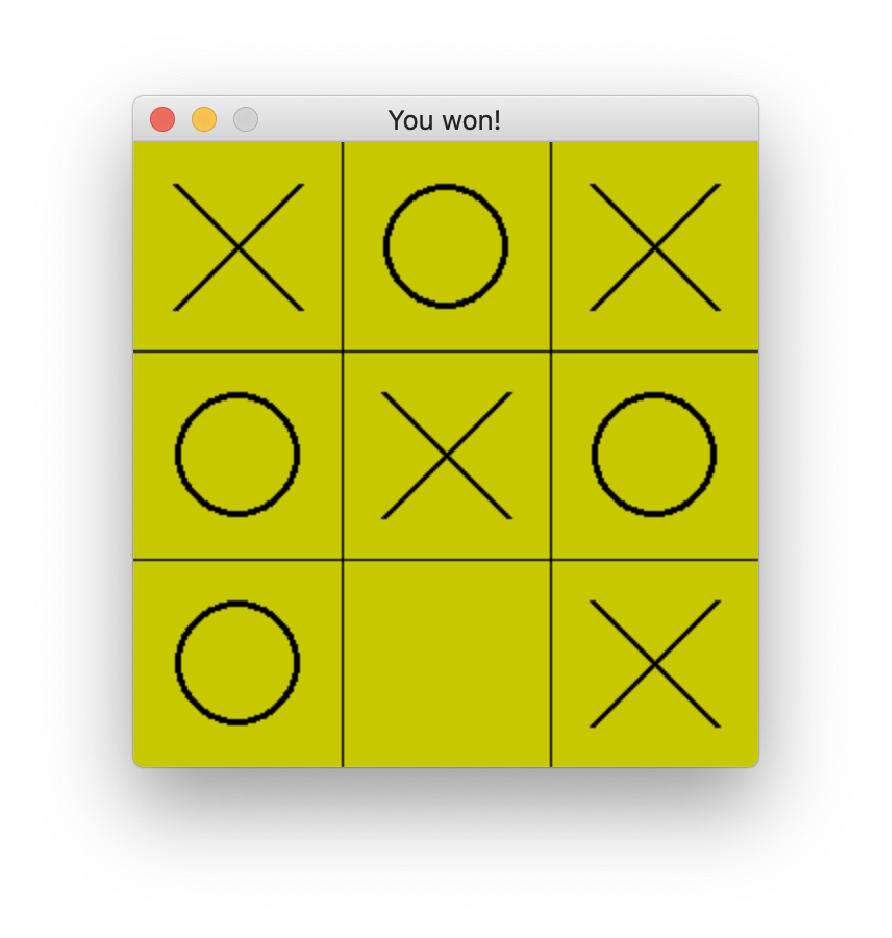
\includegraphics[width=0.4\hsize]{figures/eps/tictactoe.eps}
\end{center}

\subsubsection{Params.py}

今回は、Params.pyというファイルに、
ParamsクラスとStateクラスという、2つのクラスを定義しておきます

\begin{lstlisting}[caption=Params.py,label=prog05-1]
from enum import auto

class Params:
    HUMAN_ID = auto()
    MACHINE_ID = auto()
    EMPTY_ID = auto()

class State:
    GAME = auto()
    MACHINE_WIN = auto()
    HUMAN_WIN = auto()
    DRAW = auto()
\end{lstlisting}%

Paramsクラスには、盤面に置く石の識別情報、
HUMAN\_IDとMACHINE\_ID、及び空きスロットを識別するEMPTY\_IDの3つの識別子を持たせます

Stateクラスには、盤面の状態=ゲームの進行状況を示す定数、
即ち、GAMEはゲーム進行中の状態、
HUMAN\_WINは人が勝った状態、MACHINE\_WINはコンピュータが勝った状態、
DRAWは引き分けの状態を表す定数として保持させます

いずれのクラスも、auto()という関数を使って自動的に重複しない値を持たせることができています

auto()によって自動的に区別された値が割り振られるため、
プログラム中で変数名を参照していく以上、それらの値そのものが
どのような値なのかは知らなくても問題はありませんね

また、これらはクラス変数と呼ばれ、「クラス名.変数名」という形で使うことができて、
このクラスから導出されるオブジェクトでは共通に持っている変数になります

オブジェクト毎に持たせているオブジェクト変数「self.変数名」とは別の変数ですので、
区別して理解するようにしましょう

\subsubsection{Screenクラス}

GUIにするので、pygameでWindow画面を用意するためのScreenクラスを作ります

\begin{lstlisting}[caption=class Screen,label=prog05-1]
import pygame

class Screen:
    def __init__(self, wh=(600,600), bgcolor=(0,0,0)):
        self.WIDTH = wh[0]
        self.HEIGHT = wh[1]
        self.COLOR = bgcolor
        self.SIZE = (self.WIDTH, self.HEIGHT)
        self.surface = pygame.display.set_mode(self.SIZE)
        self.SLOTW = self.WIDTH//3
        self.SLOTH = self.HEIGHT//3

    def fill(self):
        self.surface.fill(self.COLOR)
        BLACK = (0,0,0)
        for i in range(1,3):
            startp = (0, self.SLOTH*i)
            endp = (self.WIDTH, self.SLOTH*i)
            pygame.draw.line(self.surface, BLACK, startp, endp)
            startp = (self.SLOTW*i, 0)
            endp = (self.SLOTW*i, self.HEIGHT)
            pygame.draw.line(self.surface, BLACK, startp, endp)

    def caption(self, str):
        pygame.display.set_caption(str)
\end{lstlisting}%

コンストラクタへの引数で、
盤面のサイズと背景色を受け取ることができますが、
特に指定しない場合にはデフォルト値が用いられる様にしています

三目並べは3x3のスロットを持つ盤面ですので、
そのための描画をfill()メソッドで行っています

caption()メソッドでは、引数で受け取った文字列をWindowのタイトルバーに表示できるようにしています

\subsubsection{Boardクラス}

Boardクラスは、Screenクラスを継承させるようにしていますので、
Screenクラスもプロパティやメソッドを、あたかもBoardクラスで用意したかのように使うことができます

Boardクラスのコンストラクタでは、引数で盤面のサイズ、背景色、キャプションに表示する文字列を受け取ることができるようにしていますが、
時に指定しなかった場合にデフォルト値が使われるように記述しています

Boardクラスのコンストラクタの冒頭で、Screenクラスのコンストラクタを呼び出して、Screenの初期化を実行し、
キャプションの表示、そして盤面の実態である3x3=9つのEMPTY要素を持つboardという名のリストを用意しています

また、ゲームの状態をself.stateに持たせることとし、ゲーム進行中の状態GAMEを初期状態として代入しています

\begin{lstlisting}[caption=class Board,label=prog05-1]
import pygame
from Screen import Screen
from Params import State,Params

class Board( Screen ):
    def __init__(self, wh=(300,300), color=(200,200,0), str='Tic-Tac-Toe'):
        super().__init__(wh, color)
        self.caption(str)
        self.board = [Params.EMPTY_ID for _ in range(9)]
        self.state = State.GAME

    def draw(self):
        self.fill()
        N = 3
        RADIUS = int(self.SLOTW*0.2)
        BLACK = (0,0,0)
        for ypos in range(N):
            yc = ypos * self.SLOTH + self.SLOTH // 2
            for xpos in range(N):
                xc = xpos*self.SLOTW + self.SLOTW // 2
                i = ypos * N + xpos
                if self.board[i] == Params.HUMAN_ID:
                    pygame.draw.circle(self.surface, BLACK, (xc,yc), RADIUS, 3)
                elif  self.board[i] == Params.MACHINE_ID:
                    startp = (xc - RADIUS, yc - RADIUS)
                    endp = (xc + RADIUS, yc + RADIUS)
                    pygame.draw.line(self.surface, BLACK, startp, endp, 3)
                    startp = (xc + RADIUS, yc - RADIUS)
                    endp = (xc - RADIUS, yc + RADIUS)
                    pygame.draw.line(self.surface, BLACK, startp, endp, 3)

    def winner(self):
        def scan(n1, n2, n3):
            p = self.board[n1] != 0 and \
                self.board[n1] == self.board[n2] and \
                self.board[n1] == self.board[n3]
            if p:
                if self.board[n1]==Params.HUMAN_ID:
                    self.state = State.HUMAN_WIN
                elif self.board[n1]==Params.MACHINE_ID:
                    self.state = State.MACHINE_WIN
            else:
                if not self.vacant():
                    self.state = State.DRAW
                else:
                    self.state = State.GAME
            return p
        #
        return scan(0, 1, 2) or scan(3, 4, 5) or scan(6, 7, 8) or \
               scan(0, 3, 6) or scan(1, 4, 7) or scan(2, 5, 8) or \
               scan(0, 4, 8) or scan(2, 4, 6)

    def vacant(self):
        empty = []
        for n, slot in enumerate(self.board):
            if slot == Params.EMPTY_ID:
                empty.append(n)
        return empty
\end{lstlisting}%

draw()メソッドは、盤面boardリストの状態をWindowのScreen上に描画しています

boardリストの要素がHUMAN\_IDと一致するならdraw.circle()で○を描き、
MACHINE\_IDと一致するならdraw.line()を使って×を描いています

winner()メソッドでは、ゲームの勝敗、引き分け、ゲーム進行中の判別をして、
self.stateプロパティにそれぞれの値を設定しています

winner()メソッドの中に持っているローカルなscan()関数が受け取る3つのスリット番号を見て、
boardリストの該当するスロットに入っている石が同じ識別子かどうかを判定しています

同じだったら、その石がHUMAN\_IDなのかMACHINE\_IDなのかを判別して、勝者をself.stateに設定します

違っていたら、石を置く場所が残っているかどうかを調べ、残っていないないなら引き分け、
残っているようならゲーム継続の状態だとしています

scan()が返す値がTrueなら、winnerの返す値もTrueになるので、このとき勝敗がついたという意味になります

vacant()メソッドは、CUIでも説明した空きスロットのリストを返すメソッドです

\subsubsection{Machineクラス}

Machineクラスのput\_stone()メソッドでは、
まず、空きスロットのリストを取得し、そのリスト内の要素を乱数で選んで、
boardリスト上のその位置に、MACHINE\_IDを代入しています

Trueを返した場合は石を普通に置いた場合、Falseを返すのは盤面に空きがなかった場合です

\begin{lstlisting}[caption=class Machine,label=prog05-1]
from random import randint
from Params import Params

class Machine():
    def __init__(self, name):
        self.name = name

    def put_stone(self, board):
        vacant = board.vacant()
        if not vacant:
            return False
        n = randint(0, len(vacant)-1)
        board.board[ vacant[n] ] = Params.MACHINE_ID
        return True
\end{lstlisting}%

\subsubsection{Humanクラス}

Humanクラスのput\_stone()メソッドでは、まず
空きスロットのリストを取得し、空きがないならFalseで戻ります

空きがある場合は、put\_stone()メソッドの中に、
ローカルに定義したget\_slot()関数を呼びだし、その
引数に、マウスがクリックした盤面の座標をタプルの形で渡します

get\_slot()関数は、boardやスロットのサイズを元に、
マウスがクリックしたのがどのスロット上なのかを求めて、
そのスロット番号を返しています

戻されたスロット番号が、空きスロットのリストに含まれていたなら、
boardのその場所にHUMAN\_IDを代入してTrueで戻ります

マウスでクリックしたスロット番号が、空きスロットリストに含まれていないなら、
それは、既に他の石が置かれているスロットだと言うことになりますから、
もう一度クリックでスロットを選び直して下さいという意味で、Noneを返しています

\begin{lstlisting}[caption=class Human,label=prog05-1]
from Params import Params

class Human:
    def __init__(self, name):
        self.name = name

    def put_stone(self, board, pos=(-1,-1)):
        def get_slot(xy):
            x, y = xy[0], xy[1]
            N = 3
            for ypos in range(N):
                y0 = board.SLOTH * ypos
                y1 = board.SLOTH * (ypos + 1)
                for xpos in range(N):
                    x0 = board.SLOTW * xpos
                    x1 = board.SLOTW * (xpos + 1)
                    if y0 < y < y1 and x0 < x < x1:
                        return ypos * N + xpos
            return -1
        vacant = board.vacant()
        if not vacant:
            return False
        n = get_slot(pos)
        if n in vacant:
            board.board[n] = Params.HUMAN_ID
        else:
            return None
        return True
\end{lstlisting}%

\subsubsection{Gameクラス}

Gameクラスのコンストラクタでは、引数turnに文字列を受け取り、それによって先手と後手を決めています

change\_tuen()メソッドは、手番を交代します

fine()メソッドは、このアプリケーションを終了させるときのメソッドで、Window上のQUITのエベントを受け取ったときに呼び出されます

キーボードイベントの取得部分で、MOUSEBUTTONUPを拾っており、
humanオブジェクトのput\_stone()メソッドにクリックした座標event.posを渡しています

judge()メソッドは、盤面の状態boardオブジェクトのstateプロパティの値を見て、
勝敗が決したのか、引き分けなのか、ゲーム思考の継続なのかを判定し、
ゲーム進行中の時だけTrueを、そうでない時はFalseを返しています

start()メソッドはゲームの進行そのもので、以下を繰り返しています

①キーイベントをチェックしてHUMANの手番ならこの中でHUMANがスロットを選ぶことになります
②盤面の状態を描画します
③MACHINEの手番なら、machineオブジェクトのput\_stone()メソッドを呼び出しています
④勝敗の判定をして、⑤画面を更新します

\begin{lstlisting}[caption=class Game,label=prog05-2]
import sys
import pygame
from pygame.locals import QUIT, MOUSEBUTTONUP
from Board import Board
from Human import Human
from Machine import Machine
from Params import State

class Game:
    def __init__(self, turn='human'):
        pygame.init()
        self.board = Board()
        self.human = Human('Taro')
        self.machine = Machine('Computer')
        self.turn = False if turn=='human' else True
        self.clock = pygame.time.Clock()
        self.FPS = 10

    def change_turn(self):
        self.turn = not self.turn

    def fine(self):
        pygame.quit()
        sys.exit()

    def key_event(self):
        for event in pygame.event.get():
            if event.type == QUIT:
                self.fine()
            elif event.type == MOUSEBUTTONUP:
                if not self.turn:
                    p = self.human.put_stone(self.board, event.pos)
                    if p:
                        self.change_turn()
                    elif p==False:
                        pass    # DRAW
                    else:
                        pass

    def judge(self):
        result = False
        if self.board.winner():
            if self.board.state == State.MACHINE_WIN:
                self.board.caption('Computer won the game!')
            elif self.board.state == State.HUMAN_WIN:
                self.board.caption('You won!')
        else:
            if self.board.state == State.DRAW:
                self.board.caption('Draw!')
            elif self.board.state == State.GAME:
                result = True
        return result

    def start(self):
        while True:
            self.key_event()
            self.board.draw()
            if self.turn:
                if self.machine.put_stone(self.board):
                    self.change_turn()
            self.judge()
            pygame.display.update()
            self.clock.tick(self.FPS)
\end{lstlisting}%

\subsubsection{main.py}

先手が誰なのかを、Gameクラスのコンストラクタに指示しています

\begin{lstlisting}[caption=main.py,label=prog05-3]
from Game import Game

if __name__ == '__main__':
    sente = 'human'
    game = Game( turn=sente )
    game.start()
\end{lstlisting}%

\section{MiniMax法}

ここまでコンピュータが採用してきた戦略は、「空いているスロットの中から乱数で選んだ場所に石を置く」という単純なものでした

ここでは、絶対に負けないコンピュータ、
(人が最善の手をとった場合に引き分けたとしても負けることはありません)を実現していきます

\subsection{mainの変更}

Gameクラスのインスタンスgameを生成する際、
コンストラクタへの引数で、先手は'human'か'machine'か、
コンピュータの採る戦略は乱数'random'か'minimax'かを指定するように直します

\begin{lstlisting}[caption=main.py,label=minimax00]
from Game import Game
from Params import Params

if __name__ == '__main__':
    sente = 'machine'           # 'machine' or 'human'
    senryaku = 'minimax'        # 'random' or 'minimax'
    game = Game( turn=sente, strategy=senryaku )
    game.start()
\end{lstlisting}

\subsection{Gameクラスの変更}

Gameクラスのコンストラクタにおいて、MACHINEが採る戦略を引数strategyで受け取り、
それをMachineクラスのコンストラクタに渡しています

\begin{lstlisting}[caption=Game.py,label=minimax02]
import sys
import pygame
from pygame.locals import QUIT, MOUSEBUTTONUP
from Board import Board
from Human import Human
from Machine import Machine
from Params import State

class Game:
    def __init__(self, turn='human', strategy='random'):
        pygame.init()
        self.board = Board()
        self.human = Human('Taro')
        self.machine = Machine('Computer', strategy)
        self.turn = False if turn=='human' else True
        self.clock = pygame.time.Clock()
        self.FPS = 10
    ・
    以下に変更なし
    ・
    ・
\end{lstlisting}

\subsection{Boardクラスの変更}

次の2つのメソッドは、MiniMax戦略で使うために追加します

can\_put()メソッドは、引数で受け取った番号のスロットが空いているかどうかを返します

undo()メソッドは、一旦石を置いたスロットを、元の空きスロットに戻すメソッドです

デバッグのために用意したメソッドです(完成したら不要です)

debug\_board()メソッドは、デバッグ用に現在の盤面の状態をファイル出力するメソッドです

\begin{lstlisting}[caption=Board.py,label=minimax04]
import pygame
from Screen import Screen
from Params import State,Params

class Board( Screen ):
    def __init__(self, wh=(300,300), color=(200,200,0), str='Tic-Tac-Toe'):
        ・
        変更なし
        ・
        ・
    def draw(self):
        ・
        変更なし
        ・
        ・
    def winner(self):
        ・
        変更なし
        ・
        ・
    def vacant(self):
        ・
        変更なし
        ・
        ・
    # 以下を追加
    def undo(self, n):
        self.board[n] = Params.EMPTY_ID

    def can_put(self, n):
        if self.board[n]==Params.EMPTY_ID:
            return True
        return False

    # ボードを表示する for Debug
    def debug_board(self, seq, debugstring):
        str0 = '\n('+str(seq)+')'
        tmp = []
        for i in range(9):
            if self.board[i] == Params.EMPTY_ID:
                tmp.append(' ')
            elif self.board[i] == Params.HUMAN_ID:
                tmp.append('o')
            elif self.board[i] == Params.MACHINE_ID:
                tmp.append('x')
        str1 =  '\n{0[0]}|{0[1]}|{0[2]}\t<-----\t0|1|2'\
                '\n{0[3]}|{0[4]}|{0[5]}\t<-----\t3|4|5'\
                '\n{0[6]}|{0[7]}|{0[8]}\t<-----\t6|7|8\n'.format(tmp)
        str2 = str0 + str1 + debugstring + '\n'
        with open('textfile.txt', 'a', encoding='utf-8') as f:
            f.write(str2)
\end{lstlisting}

\subsection{Machineクラスの変更}

Machineクラスのコンストラクタで、戦略が'random'か'minimax'かを受け取っています

Strategyクラスを継承しており、MiniMaxの具体的な戦略のプログラムコードは
上位クラスのStrategyに記述することにします

put\_stone()メソッドでは、
①空きスロットのリストvacantを取得し、
②空きがないなら③石を置けないのでFalseで返ります。
④strategyが'random'だった場合、
⑤乱数でvacantのインデックスnを選び、
⑥vacantのn番目にあるスロット番号に石を置きます。
⑦strategyが'minimax'だった場合、
⑧MiniMax法によるベストな手をスロット番号nで受け取り、
⑨そこに石を置きます

\begin{lstlisting}[caption=Machine.py,label=minimax06]
from random import randint
from Params import Params
from Strategy import Strategy

class Machine( Strategy ):
    def __init__(self, name, strategy):
        super().__init__()
        self.name = name
        self.strategy = strategy

    def put_stone(self, board):
        vacant = board.vacant()
        if not vacant:
            return False
        if self.strategy=='random':
            n = randint(0, len(vacant)-1)
            board.board[ vacant[n] ] = Params.MACHINE_ID
        elif self.strategy=='minimax':
            n = self.bestMove(board, vacant)
            board.board[ n ] = Params.MACHINE_ID
        return True
\end{lstlisting}

\subsection{Strategyクラスを追加}

ここにMiniMax戦略のコードをまとめて記述します

bestMove()メソッドでは、
①引数で空のスロット番号のリストvacantを受け取り、
②そのリストの要素の全てについて
③順に試して
④その手を評価していきます(MaximizerであるMachineが③で石を置いた直後ですから、次はHuman即ちMinimizerの手番ですよ、という意味でFalseを引数に指示しています)
⑤高い評価値の得られたスロット番号は、
⑥bestMoveの候補として更新していきます
⑦③で選んだ手を元の空のスロットに戻して、
③次の手を置いてみて④評価することを繰り返します

minimax() メソッドでは、
①まず、boardインスタンスのwinner()メソッドを呼んで現在の盤面の状態が、
ゲーム進行中(GAME)なのか、勝敗が決した(MACHINE\_WINかHUMAN\_WIN)のか、引き分け(DRAW)だったのかを判定します
②ゲーム進行中(GAME)でないなら、③評価関数であるローカルなevaluate()メソッドを呼びだし、結果を返します
④ゲーム進行中ならば、⑤全てのスロット番号を順に選んで、⑥そのスロットが空で石を置けるかどうかを判定し、置けるならば、
⑦そのスロットに石を置きます(Maximizer=Machine='×'か、Minimizer=Human='○'かによって置く石は違います)
⑧再帰的にminimax()メソッドを呼び出します(isMaximizingPlayerをnotとして引数に指示し、
ターンを交互に割り当てるようにしています)⑨bestValを更新していきます。⑩石を置いた番号のスロットを空に戻します

minimax()メソッドの中に定義された評価関数のevaluate()は、
ゲームが進行状態(GAME)でない場合に呼び出されるので、
Machineが勝った場合(MACHINE\_WIN)、Humanが勝った場合(HUMAN\_WIN)、
引き分けだった場合(DRAW)に、それぞれ評価値を返しています


\begin{lstlisting}[caption=Strategy.py,label=minimax07]
from Params import Params, State

class Strategy:
    INFINITY = 10000
    def __init__(self):
        pass

    def bestMove(self, board, vacant):
        bestEval = -Strategy.INFINITY
        bestMove = -1
        self.debug_seq = 0
        for n in vacant:
            board.board[n] = Params.MACHINE_ID
            eval = self.minimax(board, 0, False)
            if bestEval<eval:
                bestEval = eval
                bestMove = n
            board.undo(n)
        return bestMove

    def minimax(self, board, depth, isMaximizingPlayer):
        def evaluate(depth):
            if board.state == State.MACHINE_WIN:
                board.state = State.GAME
                return 10-depth     #return 10
            elif board.state == State.HUMAN_WIN:
                board.state = State.GAME
                return depth-10     #return -10
            else:
                self.state = State.GAME
                return 0

        board.winner()
        if board.state != State.GAME:
            return evaluate(depth)
        bestVal = -Strategy.INFINITY if isMaximizingPlayer else +Strategy.INFINITY
        for n in range(9):
            if board.can_put(n):
                board.board[n] = Params.MACHINE_ID if isMaximizingPlayer else Params.HUMAN_ID
                value = self.minimax(board, depth + 1, not isMaximizingPlayer)
                bestVal = max(value, bestVal) if isMaximizingPlayer else min(value, bestVal)
                board.undo(n)
        return bestVal
\end{lstlisting}

\section{Alpha Bata Pruning}

Alpha Beta Pruningは新しい手法のアルゴリズムではなく、MiniMax法を最適化したものにすぎません

MiniMax法は、勝敗が決着するまで全ての手を試行して、その上で最善手を選ぶため、
引き分けることはあっても負けることはありません。

しかし、全ての手を試行するというのは、多くのゲームで現実的な方法にはなりません。
三目並べの様な小規模のゲームでは、それほど問題になりませんが、リバーシなどになると
思考時間がかかりすぎて実用的ではありません

そこで、MiniMax法の試行を途中で合理的に打ち切る手法がアルファ刈りベータ刈りと呼ばれる手法です

\subsection{mainの変更}

Gameクラスのインスタンスgameを生成する際、
コンストラクタへの引数で、先手は'human'か'machine'か、
コンピュータの採る戦略は乱数'random'か'minimax'か'alphabeta'の何れかを指定するようにします

\begin{lstlisting}[caption=main.py,label=minimax00]
from Game import Game
from Params import Params

if __name__ == '__main__':
    sente = 'human'           # 'machine' or 'human'
    senryaku = 'alphabeta'        # 'random', 'minimax' or 'alphabeta'
    game = Game( turn=sente, strategy=senryaku )
    game.start()
\end{lstlisting}

\subsection{Machineクラスの変更}

戦略として、alphabetaを選べるように直します

\begin{lstlisting}[caption=class Machine,label=minimax00]
from random import randint
from Params import Params
from Strategy import Strategy

class Machine( Strategy ):
    def __init__(self, name, strategy):
        super().__init__()
        self.name = name
        self.strategy = strategy

    def put_stone(self, board):
        vacant = board.vacant()
        if not vacant:
            return False
        if self.strategy=='random':
            n = randint(0, len(vacant)-1)
            board.board[ vacant[n] ] = Params.MACHINE_ID
        elif self.strategy=='minimax':
            n = self.bestMove(board, vacant)
            board.board[ n ] = Params.MACHINE_ID
        elif self.strategy=='alphabeta':
            n = self.bestMoveAB(board, vacant)
            board.board[ n ] = Params.MACHINE_ID
        return True
\end{lstlisting}

\subsection{Strategyクラスの変更}

具体的な戦略は、こちらのクラスに記述しています

\begin{lstlisting}[caption=class Strategy,label=minimax00]
from Params import Params, State

class Strategy:
    INFINITY = 10000
    def __init__(self):
        pass

    def bestMove(self, board, vacant):
            ・
            変更なし
            ・
            ・

    def minimax(self, board, depth, isMaximizingPlayer):
            ・
            変更なし
            ・
            ・

    def bestMoveAB(self, board, vacant):
        bestEval = -Strategy.INFINITY
        bestMove = -1
        for n in vacant:
            board.board[n] = Params.MACHINE_ID
            eval = self.minimaxab(board, 0, 0, False, -Strategy.INFINITY, +Strategy.INFINITY)
            if bestEval<eval:
                bestEval = eval
                bestMove = n
            board.undo(n)
        return bestMove

    def minimaxab(self, board, node, depth, isMaximizingPlayer, alpha, beta):
        def evaluate(depth):
            if board.state == State.MACHINE_WIN:
                board.state = State.GAME
                return 10-depth     #return 10
            elif board.state == State.HUMAN_WIN:
                board.state = State.GAME
                return depth-10     #return -10
            else:
                self.state = State.GAME
                return 0

        board.winner()
        if board.state != State.GAME:
            return evaluate(depth)

        bestVal = -Strategy.INFINITY if isMaximizingPlayer else +Strategy.INFINITY
        for n in range(9):
            if board.can_put(n):
                board.board[n] = Params.MACHINE_ID if isMaximizingPlayer else Params.HUMAN_ID
                value = self.minimaxab(board, node+1, depth+1, not isMaximizingPlayer, alpha, beta)
                board.undo(n)
                if isMaximizingPlayer:
                    bestVal = max(value, bestVal)
                    alpha = max(alpha, bestVal)
                else:
                    bestVal = min(value, bestVal)
                    beta = min(beta, bestVal)
                if beta<=alpha:
                    #print('depth=',depth)
                    break
        return bestVal
\end{lstlisting}

%\chapter{連珠(五目並べ Connect Four)}

\chapter{リバーシ(オセロ):N $\times$ N}
8 $\times$ 8サイズのゲームが一般的ですが、
6 $\times$ 6盤の縮小リバーシでは必勝法が見つかっているようです

1993年にイギリスのJoel Feinsteinが、6 $\times$ 6盤の縮小リバーシで、
先手が最善手を尽くしたとしても後手が「20対16」で勝つ、
(先手16対、後手20で、後手の4目勝ち)という事を示したということです

ここでは、
4 $\times$ 4「以上」の大きさの盤面に対応するリバーシを作ります。
あなたにゲームを最後まで続ける根気があるなら、
10 $\times$ 10でも20 $\times$ 20でもゲームすることができるかもしれません

\section{CUI版}

以下のゲーム例では、×(BLACK)の手番ですが、○(WHITE)を裏返せないところに×を置こうとしたり、
×(BLACK)を置ける場所があるのにpassを宣言したりすると、再入力を促されています

○(WHITE)の手番で、まずは乱数によってコンピュータが石を置くスロットを決めていますが、
後ほどStrategyクラスで、コンピュータの強い戦略について考察していきます

\begin{spacing}{0.74}
\begin{verbatim}
  WHITE:2, BLACK:2
    0 1 2 3 →x
  0 . . . .
  1 . X O .
  2 . O X .
  3 . . . .
  ↓
  y
  Your turn. [yx] or "pass": 23
  Your turn. [yx] or "pass": pass
  Your turn. [yx] or "pass": 13

  WHITE:1, BLACK:4
    0 1 2 3 →x
  0 . . . .
  1 . X X X
  2 . O X .
  3 . . . .
  ↓
  y
  WHITE:3, BLACK:3
    0 1 2 3 →x
  0 . . . .
  1 . X X X
  2 . O O O
  3 . . . .
  ↓
  y
  Your turn. [yx] or "pass": 33

  WHITE:1, BLACK:6
    0 1 2 3 →x
  0 . . . .
  1 . X X X
  2 . O X X
  3 . . . X
  ↓
  y
  WHITE:3, BLACK:5
    0 1 2 3 →x
  0 . O . .
  1 . O X X
  2 . O X X
  3 . . . X
  ↓
  y
  Your turn. [yx] or "pass": 00

  ( ・・ 途中略 ・・ )

  WHITE:5, BLACK:9
    0 1 2 3 →x
  0 X X X O
  1 O X X X
  2 O O X X
  3 O . . X
  ↓
  y
  Your turn. [yx] or "pass": 31

  WHITE:4, BLACK:11
    0 1 2 3 →x
  0 X X X O
  1 O X X X
  2 O X X X
  3 O X . X
  ↓
  y
  WHITE:7, BLACK:9
    0 1 2 3 →x
  0 X X X O
  1 O X X X
  2 O O X X
  3 O O O X
  ↓
  y

  Winner : BLACK
\end{verbatim}
\end{spacing}

\newpage

\subsection{Human vs. Machine}

\subsubsection{Gameクラス}

メインでは、Gameクラスのコンストラクタでへの引数で盤面のサイズ(N=4以上の偶数)、
先手を'human', 'machine'から、戦略を'random', 'maxflip', 'minimax', 'alphabeta'から指定します

\begin{lstlisting}[caption=main,label=othello00]
from Game import Game

if __name__ == '__main__':
    sente = 'human'         # 'human, 'machine'
    senryaku = 'maxflip'    # 'random', 'maxflip', 'minimax', 'alphabeta'
    game = Game( N=6, turn=sente, strategy=senryaku )      # board size -> N x N
    game.start()
\end{lstlisting}

Gameクラスのコンストラクタで、盤面クラス(Board)のインスタンス(board)、
人クラス(Human)のインスタンス(human)、
コンピュータクラス(Machine)のインスタンス(machine)を生成し、
インスタンス変数self.playerには、humanとmachineの2つのインスタンスを要素とするリストを用意しています

start()メソッドで、ゲームの進行の主要部分を記述しています

①盤面を印刷(board.print())し、②プレーヤの打つ手を選び(player[turn].Te(self.board))、
③もし、パス(Board.PASS)でなかった場合は、④盤面に石を置く(board.putStone(te,color))
ことになります。
⑤パスならば盤面に石を置かずに、プレーヤを交代(turn = (turn+1)\%2)します

⑥盤面の状況から勝敗の判定(board.Winner())を行い、戻り値が
Board.GAMEならばゲームを継続、それ以外
(BLACK\_WINかWHITE\_WINかDRAW)ならば、ゲームを終了して結果の勝敗を表示します

\begin{lstlisting}[caption=Game class,label=othello01]
from Board import Board
from Human import Human
from Machine import Machine
from Stone import Stone

class Game():
    def __init__(self, N=4, turn='human', strategy='random'):
        self.board = Board(NW=N)
        human = Human(color=Stone.BLACK)
        machine = Machine(color=Stone.WHITE, strategy=strategy)
        self.player = [human, machine]
        self.turn = 0
        if turn=='machine':
            self.turn = 1

    def start(self):
        turn = self.turn
        winner = Board.GAME
        while winner==Board.GAME:
            self.board.print()                    # ①

            te = self.player[turn].Te(self.board) # ②
            if te!=Board.PASS:                    # ③
                color = self.player[turn].color
                self.board.put_stone(te,color)    # ④

            turn = (turn+1)%2                     # ⑤
            winner = self.board.winner()          # ⑥

        self.board.print()
        print()
        if winner==Board.BLACK_WIN:
            print('Winner : BLACK')
        elif winner==Board.WHITE_WIN:
            print('Winner : WHITE')
        elif winner==Board.DRAW:
            print('DRAW')
\end{lstlisting}

\subsubsection{Stoneクラス}

石のクラスでは、BLACK、WHITE、EMPTYの中の何れかの色特性(self.color)、
及び盤面上の位置(self.locate)をプロパティとして持たせています

用意しているメソッドは、各プロパティに関するセッターやゲッターです

\begin{lstlisting}[caption=Stone class,label=othello04]
class Stone():
    EMPTY = 0
    BLACK = 1
    WHITE = 3 - BLACK
    MACHINE_ID = WHITE
    HUMAN_ID = BLACK
    def __init__(self, te, color):
        self.color = color
        self.locate = te

    def getLocate(self):
        return self.locate

    def setColor(self, color):
        self.color = color

    def getColor(self):
        return self.color

    def flipColor(self):
        self.color = 3 - self.color

    def getFigure(self):
        if self.color==Stone.BLACK:
            return 'X'
        elif  self.color==Stone.WHITE:
            return 'O'
        return '.'
\end{lstlisting}

\subsubsection{Boardクラス}

このクラスでは、盤面の状態をリスト(self.stones)に保持しています

コンストラクタでは、
まず引数で示されたサイズ(NW * NW)の空の(Stone.EMPTY)盤面を用意しています

次に、盤面の中央にBLACKとWHITEの石をそれぞれ2個ずつ配置しますが、
配置のパタンは乱数によって決めています

石の数を nWhite,nBlack,nEmpty に保持させ、
winner()メソッドの最初でそれぞれの値を数えています

nWhite+nBlack+nEmptyは盤面のスロットの総数になりますから、
nEmptyがゼロになった段階で、nWhiteとnBlackの大小関係から
勝敗を決定しています
(nEmptyがゼロになるより前に勝敗の判定がつく場合について、
具体的にプログラムする必要があるかもしれません)

print()メソッドは、画面に盤面の状態を表示しています

is\_empty()メソッドは、引数で指定したスロットが空(Stone.EMPTY)
であるか否かを判定しています

empty\_list()メソッドは、現在の盤面において、
空(Stone.EMPTY)のスロット番号の一覧をリストにして返します

can\_put(te, color)メソッドは、引数teで示されたスロット番号の場所に、
第2引数のcolorで示された色の石を置けるかどうかを判定しています
(具体的には、self.check\_flip( Stone(te, color) )を呼び出して、
色を反転できる石が何個かあるなら、そこには石を置けるという判断をしています)

check\_flip(stone)メソッドでは、
引数で受け取っているstoneオブジェクトは、その石を置こうとしているスロットの位置番号、
及びその石の色をプロパティとして持っていますから、盤面のその位置に指定された色の
石を置いたときに、上下、左右、右斜め上、右斜め下、左斜め上、左斜め下の8つの方向で
何個の石を反転できるかを数えています(最後に、反転できる石の総数を返しています)

flip\_list(stone)メソッドでは、
check\_flip(stone)メソッドで数えた各方向での反転できる石の数に基づいて、
反転する石のスロット番号のリストを作って返しています

put\_stone(te, color)メソッドは、
まずは、指定されたスロット位置に指定の石を置いた後に、
反転する石のリストをflip\_list(stone)メソッドで作って、
そのリストをset\_stones(flist,color)に渡して、
実際に盤面の石を反転させるようにします

set\_stones(flist,color)メソッドは、受け取ったリストを基に
盤面のデータを更新し、石を反転させています

reset\_stones()メソッドは、
set\_stones()メソッドで反転させた盤面上の石を元に戻します

puttable()メソッドは、can\_put()メソッドがTrueだった場合のnKomaリストを取得します

puttable\_list()メソッドは、puttbale()メソッドの戻り値から、
盤面上で石を置ける場所のリストを取得します

\begin{lstlisting}[caption=Board class,label=othello05]
from random import randint
from Stone import Stone

class Board:
    PASS = -10
    GAME =  -1
    DRAW =   0
    HUMAN_WIN = BLACK_WIN = Stone.BLACK * 100
    MACHINE_WIN = WHITE_WIN = Stone.WHITE * 100
    UNITV = ((0,-1),(1,-1),(1,0),(1,1),(0,1),(-1,1),(-1,0),(-1,-1))

    def __init__(self, NW=4):
        self.nKoma = [0 for _ in range(9)]
        self.NW = NW
        self.NxN = NW * NW
        self.stones = [ Stone(i, Stone.EMPTY) for i in range(self.NxN) ]
        m = NW//2
        n = m - 1
        self.stones[NW*n+n].setColor( Stone.WHITE )
        self.stones[NW*n+m].setColor( Stone.BLACK )
        self.stones[NW*m+n].setColor( Stone.BLACK )
        self.stones[NW*m+m].setColor( Stone.WHITE )
        nrnd = randint(0,1)
        if nrnd==0:
            self.stones[NW * n + n].flipColor()
            self.stones[NW * n + m].flipColor()
            self.stones[NW * m + n].flipColor()
            self.stones[NW * m + m].flipColor()
        self.nBlack = self.nWhite = 2
        self.nEmpty = self.NxN - (self.nBlack + self.nWhite)
        self.state = Board.GAME

    def winner(self):
        self.nBlack = self.nWhite = self.nEmpty = 0
        for i in range(self.NxN):
            if self.stones[i].getColor() == Stone.HUMAN_ID:
                self.nBlack += 1
            elif self.stones[i].getColor() == Stone.MACHINE_ID:
                self.nWhite += 1
            else:
                self.nEmpty += 1
        if self.nBlack+self.nWhite == self.NxN:
            if self.nBlack < self.nWhite:
                return Board.MACHINE_WIN
            elif self.nBlack > self.nWhite:
                return Board.HUMAN_WIN
            else:
                return Board.DRAW
        return Board.GAME

    def print(self):
        print(f"WHITE:{self.nWhite}, BLACK:{self.nBlack}")
        print(' ',end=' ')
        for x in range(self.NW):
            print(f"{x}", end=' ')
        print("→x")
        for y in range(self.NW):
            print(f"{y:}", end=' ')
            for x in range(self.NW):
                print(f"{self.stones[ y*self.NW+x ].getFigure()}", end=' ')
            print()
        print("↓\ny")

    def check_flip(self, stone):
        y = stone.getLocate()//self.NW
        x = stone.getLocate()%self.NW
        self.nKoma[8] = 0
        if self.stones[y*self.NW+x].getColor() == Stone.EMPTY:
            for i1 in range( len(self.nKoma)-1 ):   # 0,1,2,3,4,5,6,7
                m1, m2 = x, y
                self.nKoma[i1] = s = ct = 0
                while s<2:
                    m1 += Board.UNITV[i1][0]
                    m2 += Board.UNITV[i1][1]
                    if (0<=m1<self.NW) and (0<=m2<self.NW):
                        color = self.stones[m2*self.NW+m1].getColor()
                        if color==Stone.EMPTY:
                            s = 3
                        elif color==stone.getColor():
                            s=2 if s==1 else 3
                        else:
                            s=1
                            ct += 1
                    else:
                        s=3
                if s==2:
                    self.nKoma[8] += ct
                    self.nKoma[i1] = ct
        return self.nKoma[8]

    def flip_list(self, stone):
        self.check_flip(stone)
        y = stone.getLocate()//self.NW
        x = stone.getLocate()%self.NW
        flipped = []
        for i1 in range( len(self.nKoma)-1 ):   # 0,1,2,3,4,5,6,7
            m1, m2 = x, y
            for i2 in range( self.nKoma[i1] ):
                m1 += Board.UNITV[i1][0]
                m2 += Board.UNITV[i1][1]
                if (0 <= m1 < self.NW) and (0 <= m2 < self.NW):
                    z = m2*self.NW+m1
                    self.stones[z].setColor( stone.getColor() )
                    flipped.append( z )
        z = y*self.NW+x
        self.stones[z].setColor( stone.getColor() )
        flipped.append(z)
        return flipped

    def empty_list(self):
        list = [v for v in range(self.NxN) if self.is_empty(v)]
        return list

    def is_empty(self, te):
        return True if self.stones[te].getColor()==Stone.EMPTY else False

    def can_put(self, te, color):
        if 0<=te<self.NxN:
            if 0<self.check_flip( Stone(te, color) ):
                return True
        return False

    def puttable(self, te, color):
        if self.can_put(te, color):
            return self.nKoma

    def puttable_list(self, color):
        emptyl = self.empty_list()
        komal = []
        telist = []
        for n in emptyl:
            w = self.puttable(n, color)
            if w:
                telist.append(n)
                komal.append(w)
        return telist, komal

    def put_stone(self, te, color):
        stone = Stone(te, color)
        flist = self.flip_list( stone )
        self.set_stones(flist, color)
        self.stones[te] = stone
        if color==Stone.BLACK:
            self.nBlack = len(flist) + 1
        else:
            self.nWhite = len(flist) + 1
        return flist

    def set_stones(self, flist, color):
        for z in flist:
            self.stones[z] = Stone(z, color)
        self.stones[z] = Stone(z, Stone.EMPTY)

    def reset_stones(self, te, flist, color):
        if color==Stone.WHITE:
            c = Stone.BLACK
        elif color==Stone.BLACK:
            c = Stone.WHITE
        self.stones[te] = Stone(te,c)
        for z in flist:
            self.stones[z] = Stone(z, c)
        self.stones[z] = Stone(z, Stone.EMPTY)

    def debug_print(self):
        for y in range(self.NW):
            for x in range(self.NW):
                n = y*self.NW + x
                print(self.stones[n].color, end=' ')
            print()
        print('\n')
\end{lstlisting}

\subsubsection{Humanクラス}

人の打つ石の手を決めているのは、このクラスのメソッドTe()です

プロンプトメッセージ('Your turn. [yx] or "pass": ')を表示して、
入力文字列を受け取ります(instr)

入力文字列(instr)の中に文字列'pass'が含まれていたなら、まず、
石を置ける場所があったにもかかわらず、誤ってパスを指示したかもしれない
可能性をチェック(puttable())します

もし、石を置く場所がある局面なら、パスをしてはいけないので、
プロンプトメッセージまで処理を戻します(continue)

石を置く場所がなくてパスの指示をしたのなら、
パスの指示を返します(return Board.PASS)

入力文字列にスロット番号として、行番号yと列番号xが[yx]として指定されたならば、
yxという2桁の数字文字を、それぞれ整数に変換(serial\_num())しています

yとxが数字から整数値に変換できたなら、スロットの位置番号を計算
(slot = cy * board.NW + cx)できます

計算したスロット番号に、その石を置けるかどうかをチェック
(board.can\_put(slot, self.color))して、置けない場合は
最初の文字列入力プロンプトまで処理を戻します

チェックした結果、石を置くことのできるスロット番号だったなら、
反復(while True)を抜けて(break)、そのスロット番号を返します(return slot)

\begin{lstlisting}[caption=Human class,label=othello03]
from Board import Board
from Stone import Stone

class Human:
    def __init__(self, color=Stone.BLACK):
        self.color = color

    def Te(self, board):
        def puttable():
            elist =  board.empty_list()
            for v in elist:
                if board.can_put(v, self.color):
                    return True
            return False

        while True:
            instr = input('Your turn. [yx] or "pass": ')
            if 'pass' in instr:
                if puttable():
                    continue
                return Board.PASS
            if 1<len(instr) and self.numP( instr[0] ) and self.numP( instr[1] ):
                cy = self.serial_num( instr[0] )
                cx = self.serial_num( instr[1] )
                slot = cy * board.NW + cx
                if board.can_put(slot, self.color):
                    break
        print()
        return slot

    def numP(self, xy):
        if '0' <= xy <= '9':
            return True
        return False

    def serial_num(self, xy):
        def fromA(xy):
            return int(xy - 'a')

        if self.numP(xy):
            nxy = int( xy )
        else:
            nxy = fromA(xy)+10
        return nxy
\end{lstlisting}

\subsubsection{Machineクラス}

コンピュータ(Machine)の打つ手を決めているのが、このクラスのメソッド、Te()です

①まず最初に、board.puttable\_list()によって石を置ける場所の一覧をtelistというリストとして取得します

②打つ手のリストの要素がない場合は、Board.PASSを返します

③打つ手のリストの要素が一つしかない場合は、迷うことなくその手を返します

④'random'戦略が選ばれている場合は、telistの中から乱数で選んだ手を返します

⑤'maxflip'戦略が選ばれている場合は、BoardクラスのnKomaリストの一番最後の要素に、
反転できる石の数の総数が入っているので、最も多く反転できる手を返します

⑥'minimax'戦略が選ばれている場合は、MINIMAX法による手が選ばれますが、
MINIMAX法は、勝敗がつくまで、最後まで対戦を試行するので、盤面のサイズが
最小値(N=4)の場合でも、とても応答に時間がかかります。

⑦'alphabeta'戦略が選ばれている場合は、MINIMAX法を途中で打ち切る手立てを
含んでいるので、多少高速な応答を期待できますが、、、、、

\begin{lstlisting}[caption=Machine class,label=othello02]
from random import randint
from Board import Board
from Stone import Stone
from Strategy import Strategy

class Machine( Strategy ):
    def __init__(self, color=Stone.WHITE, strategy = 'random'):
        self.color = color
        self.strategy = strategy

    def Te(self, board):
        telist, komalist = board.puttable_list( self.color )
        if not telist:
            return Board.PASS
        if len(telist)==1:
            return telist[0]
        if self.strategy == 'random':
            n = randint( 0, len(telist)-1 )
            return telist[n]
        elif self.strategy == 'maxflip':
            n = v = -1
            for i, k in enumerate(komalist):
                if n < k[-1]:
                    n = k[-1]
                    v = telist[i]
            return v
        elif self.strategy == 'minimax':
            print('thinking ...')
            n = self.bestMove(board, telist)
            print('Your turn.')
            return n
        elif self.strategy == 'alphabeta':
            n = self.bestMoveAB(board, telist)
            return n
\end{lstlisting}

\subsection{Machineの戦略:Strategyクラス}

このクラスは、Machineクラスのスーパークラスとして、
Machineクラスに継承させて使うようにします

ここには、MINIMAX法とAlpha-Beta刈りの2つを記述しています

\begin{lstlisting}[caption=Strategy class,label=othello06]
from Board import Board
from Stone import Stone

class Strategy:
    INFINITY = 100000
    def __init__(self):
        pass

    # MiniMax
    def bestMove(self, board, telist):
        bestEval = -Strategy.INFINITY
        bestMove = -1
        for n, v in enumerate(telist):
            flist = board.put_stone(v, self.color)
            eval = self.minimax(board, 0, False)
            if bestEval<eval:
                bestEval = eval
                bestMove = v
            board.reset_stones(v, flist, self.color)
        return bestMove

    def minimax(self, board, depth, isMaximizingPlayer):
        def evaluate(depth):
            if board.state == Board.MACHINE_WIN:
                board.state = Board.GAME
                return board.NxN-depth     #return NxN
            elif board.state == Board.HUMAN_WIN:
                board.state = Board.GAME
                return depth-board.NxN     #return -NxN
            else:
                self.state = Board.GAME
                return 0

        board.winner()
        if board.state != Board.GAME:
            return evaluate(depth)

        color = Stone.MACHINE_ID if isMaximizingPlayer else Stone.HUMAN_ID
        telist, _ = board.puttable_list(color)
        bestVal = -Strategy.INFINITY if isMaximizingPlayer else +Strategy.INFINITY
        for n, v in enumerate(telist):
            flist = board.put_stone(v, color)
            value = self.minimax(board, depth + 1, not isMaximizingPlayer)
            bestVal = max(value, bestVal) if isMaximizingPlayer else min(value, bestVal)
            board.reset_stones(v, flist, color)
        return bestVal

    # Alpha-Beta
    def bestMoveAB(self, board, telist):
        bestEval = -Strategy.INFINITY
        bestMove = -1
        for n, v in enumerate(telist):
            flist = board.put_stone(v, self.color)
            eval = self.minimaxab(board, 8, 0, False, -Strategy.INFINITY, +Strategy.INFINITY)
            if bestEval<eval:
                bestEval = eval
                bestMove = v
            board.reset_stones(v, flist, self.color)
        return bestMove

    def minimaxab(self, board, node, depth, isMaximizingPlayer, alpha, beta):
        def evaluate(depth):
            if board.state == Board.MACHINE_WIN:
                board.state = Board.GAME
                return board.NxN-depth     #return NxN
            elif board.state == Board.HUMAN_WIN:
                board.state = Board.GAME
                return depth-board.NxN     #return -NxN
            else:
                self.state = Board.GAME
                return 0

        board.winner()
        if board.state != Board.GAME:
            return evaluate(depth)
        elif node==0:
            n = board.nBlack - board.nWhite
            return n if isMaximizingPlayer else -n

        color = Stone.MACHINE_ID if isMaximizingPlayer else Stone.HUMAN_ID
        telist, _ = board.puttable_list(color)
        bestVal = -Strategy.INFINITY if isMaximizingPlayer else +Strategy.INFINITY
        for n, v in enumerate(telist):
            flist = board.put_stone(v, color)
            value = self.minimaxab(board, node-1, depth+1, not isMaximizingPlayer, alpha, beta)
            board.reset_stones(v, flist, color)
            if isMaximizingPlayer:
                bestVal = max(value, bestVal)
                alpha = max(alpha, bestVal)
            else:
                bestVal = min(value, bestVal)
                beta = min(beta, bestVal)
            if beta<=alpha:
                break
        return bestVal
\end{lstlisting}

【演習】GUI版に直してみましょう

\section{GUI版}

人とコンピュータの対戦をGUI化します

コンピュータがPASSの局面では、人の手番になるだけですが、
人がPASSの判断をする局面では、何らかの方法でその旨を知らせてやる必要があります。
真ん中の4つのスロットは空きになることはないので、
その4つのどれかをクリックしたときにはPASSを選択したことにします。
ただし、人がPASSを選択してもどこかに石を置けるようでしたら、
手番は交代せず、石を置けるスロットがクリックするのを待っています。

利口な戦略を選ぼうとすると、盤面のサイズとの兼ね合いで実用的なゲームにならないことがあります。
StrategyクラスやMachineクラスを見て、そこで行っている処理を研究してみてください

\begin{center}
  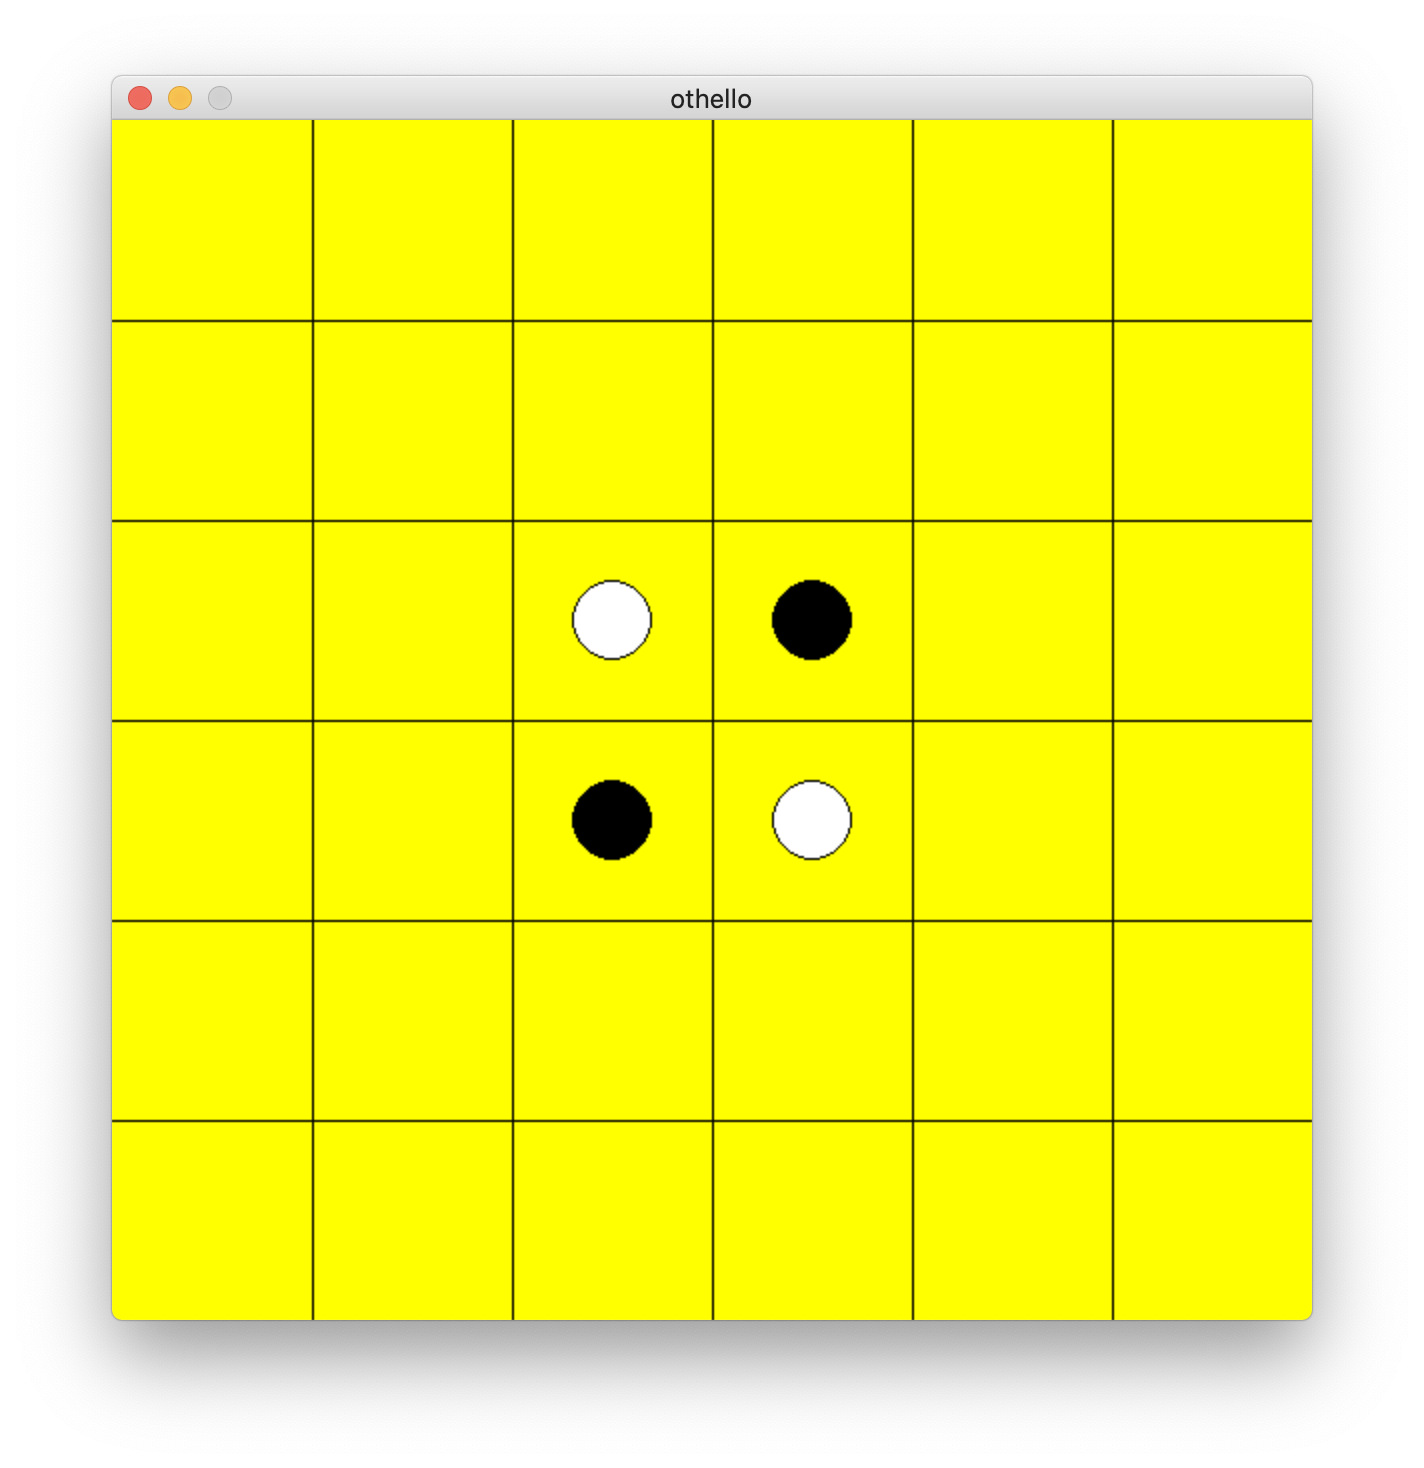
\includegraphics[width=0.5\hsize]{figures/eps/othello.eps}
\end{center}

\subsubsection{main.pyに変更なし}

メインに変更はありません。Gameクラスのコンストラクタでへの引数で盤面のサイズ(N=4以上の偶数)、
先手を'human', 'machine'から、戦略を'random', 'maxflip', 'minimax', 'alphabeta'から指定します

\begin{lstlisting}[caption=main,label=othello00]
from Game import Game

if __name__ == '__main__':
    sente = 'human'         # 'human, 'machine'
    senryaku = 'maxflip'    # 'random', 'maxflip', 'minimax', 'alphabeta'
    game = Game( N=6, turn=sente, strategy=senryaku )      # board size -> N x N
    game.start()
\end{lstlisting}

\subsubsection{Screenクラスの追加}

\begin{lstlisting}[caption=Screen class,label=othello07]
import pygame

class Screen:
    def __init__(self, NW=4, wh=(600, 600), bgcolor=(0, 0, 0)):
        self.NW = NW
        self.WIDTH = wh[0]
        self.HEIGHT = wh[1]
        self.COLOR = bgcolor
        self.SIZE = (self.WIDTH, self.HEIGHT)
        self.surface = pygame.display.set_mode(self.SIZE)
        self.SLOTW = self.WIDTH // NW
        self.SLOTH = self.HEIGHT // NW

    def fill(self):
        self.surface.fill(self.COLOR)
        BLACK = (0, 0, 0)
        for i in range(1, self.NW):
            startp = (0, self.SLOTH * i)
            endp = (self.WIDTH, self.SLOTH * i)
            pygame.draw.line(self.surface, BLACK, startp, endp)
            startp = (self.SLOTW * i, 0)
            endp = (self.SLOTW * i, self.HEIGHT)
            pygame.draw.line(self.surface, BLACK, startp, endp)

    def caption(self, str):
        pygame.display.set_caption(str)
\end{lstlisting}

\subsubsection{Boardクラスの書き換え}

Boardクラスは、Screenクラスを継承させることとし、
Boardクラスのコンストラクタの冒頭で、
Screenクラスのコンストラクタを呼び出すようにします

盤面をsurfaceに描画するメソッド、draw()をBoardクラスの最後に追加します。
draw()メソッドでは、self.stonesのリストに持っている石の色に従って、
白丸と黒丸をpygame.draw.circle()を使って描いています

\begin{lstlisting}[caption=Board class,label=othello08]
from random import randint
import pygame
from Stone import Stone
from Screen import Screen

class Board( Screen ):    # Screenを継承するように変更
    PASS = -10
    GAME =  -1
    DRAW =   0
    HUMAN_WIN = BLACK_WIN = Stone.BLACK * 100
    MACHINE_WIN = WHITE_WIN = Stone.WHITE * 100
    UNITV = ((0,-1),(1,-1),(1,0),(1,1),(0,1),(-1,1),(-1,0),(-1,-1))

    def __init__(self, NW=4):
        # Screenのコンストラクタ呼びだしを追加
        super().__init__( NW=NW, wh=(600,600), bgcolor=(255,255,0) )
        # コンストラクタの以下の部分に変更なし
        self.nKoma = [0 for _ in range(9)]
        self.NW = NW
        self.NxN = NW * NW
        self.stones = [ Stone(i, Stone.EMPTY) for i in range(self.NxN) ]
        m = NW//2
        n = m - 1
        self.stones[NW*n+n].setColor( Stone.WHITE )
        self.stones[NW*n+m].setColor( Stone.BLACK )
        self.stones[NW*m+n].setColor( Stone.BLACK )
        self.stones[NW*m+m].setColor( Stone.WHITE )
        nrnd = randint(0,1)
        if nrnd==0:
            self.stones[NW * n + n].flipColor()
            self.stones[NW * n + m].flipColor()
            self.stones[NW * m + n].flipColor()
            self.stones[NW * m + m].flipColor()
        self.nBlack = self.nWhite = 2
        self.nEmpty = self.NxN - (self.nBlack + self.nWhite)
        self.state = Board.GAME

    def winner(self):
        ・
        ・
        変更なし
        ・
        ・

    # 以下を、Boardクラスの最後に追加

    def draw(self):
        self.fill()
        N = self.NW
        RADIUS = int(self.SLOTW*0.2)
        BLACK = (0,0,0)
        for ypos in range(N):
            yc = ypos * self.SLOTH + self.SLOTH // 2
            for xpos in range(N):
                xc = xpos*self.SLOTW + self.SLOTW // 2
                i = ypos * N + xpos
                if self.stones[i].getColor() == Stone.WHITE:
                    pygame.draw.circle(self.surface, (255,255,255), (xc,yc), RADIUS)
                    pygame.draw.circle(self.surface, BLACK, (xc, yc), RADIUS, 1)
                elif  self.stones[i].getColor() == Stone.BLACK:
                    pygame.draw.circle(self.surface, BLACK, (xc, yc), RADIUS)
\end{lstlisting}

\subsubsection{Gameクラスの書き換え}

start()メソッドの中で、Machineが石を置くときの処理を書き、
key\_event()メソッドの中で、MOUSEBUTTONUPのイベントを拾ったときに
Humanが盤面上に石を置く時の処理を書いています

windowのcaptionへの文字列の表示が効果的なものになるように、
工夫してみましょう

\begin{lstlisting}[caption=Game class,label=othello09]
import sys
import pygame
from pygame.locals import QUIT, MOUSEBUTTONUP
from Board import Board
from Human import Human
from Machine import Machine
from Stone import Stone

class Game():
    def __init__(self, N=4, turn='human', strategy='random'):
        pygame.init()
        self.board = Board( NW=N )
        self.board.caption('othello')
        self.human = Human(color=Stone.BLACK)
        self.machine = Machine(color=Stone.WHITE, strategy=strategy)
        self.turn = False if turn == 'human' else True
        self.clock = pygame.time.Clock()
        self.FPS = 10

        def key_event(self):
            def fine():
                pygame.quit()
                sys.exit()
            for event in pygame.event.get():
                if event.type == QUIT:
                    fine()
                elif event.type == MOUSEBUTTONUP:
                    if not self.turn:
                        self.board.caption('Your turn')
                        p = self.human.put_stone(self.board, event.pos)
                        if p==True or p==Board.PASS:
                            self.turn = not self.turn
                            self.board.caption('Machine turn')
                        else:
                            pass        # DRAW

    def judge(self):
        result = False
        self.board.winner()
        if self.board.state == Board.MACHINE_WIN:
            self.board.caption('Computer won the game!')
        elif self.board.state == Board.HUMAN_WIN:
            self.board.caption('You won!')
        elif self.board.state == Board.DRAW:
            self.board.caption('Draw!')
        else:
            #self.board.state == Board.GAME:
            result = True
        return result

    def start(self):
        while True:
            self.key_event()
            self.board.draw()
            if self.turn:
                self.board.caption('Machine turn')
                p = self.machine.put_stone(self.board)
                if p==True or p==Board.PASS:
                    self.turn = not self.turn
                    self.board.caption('Your turn')
            self.judge()
            pygame.display.update()
            self.clock.tick(self.FPS)
\end{lstlisting}

\subsubsection{Machineクラスの書き換え}

Machineクラスの最後にput\_stone()メソッドを追加しますが、
内容は、CUIの時のTe()メソッドを呼び出しているだけです

\begin{lstlisting}[caption=Machine class,label=othello10]
from random import randint
from Board import Board
from Stone import Stone
from Strategy import Strategy

class Machine( Strategy ):
    def __init__(self, color=Stone.WHITE, strategy = 'random'):
        self.color = color
        self.strategy = strategy

    def Te(self, board):
        ・
        ・
        変更なし
        ・
        ・

    # 以下を、Machineクラスの最後に追加

    def put_stone(self, board):
        board.caption('thinking....')
        te = self.Te(board)
        if te!=board.PASS:
            board.put_stone(te, self.color)
            return True
        return Board.PASS
\end{lstlisting}

\subsubsection{Humanクラスの書き換え}

Humanクラスでは、Gameクラスの中から呼び出される、
put\_stone()メソッドを追加します

put\_stone()メソッドでは、マウスボタンを離したイベントで受け取った
screen上の座標値をposという名のタプルで受け取りますので、
その座標がオセロ盤の何番のスロットをクリックしたのかを導出しています

また真ん中の4つのスロットは、PASSを指示するためのスロットでもあるので、
その判定もしています

Falseを返す場合というのは、
「もう一度呼びだし直してください」という意味になります

\begin{lstlisting}[caption=Human class,label=othello11]
from Board import Board
from Stone import Stone

class Human:
    def __init__(self, color=Stone.BLACK):
        self.color = color

    def Te(self, board):
        ・
        ・
        変更なし
        ・
        ・

    # 以下を、Humanクラスの最後に追加

    def put_stone(self, board, pos=(-1,-1)):
        def get_slot(xy):
            x, y = xy[0], xy[1]
            N = board.NW
            for ypos in range(N):
                y0 = board.SLOTH * ypos
                y1 = board.SLOTH * (ypos + 1)
                for xpos in range(N):
                    x0 = board.SLOTW * xpos
                    x1 = board.SLOTW * (xpos + 1)
                    if y0 < y < y1 and x0 < x < x1:
                        return ypos * N + xpos
            return -1
        nw = board.NW
        nwc = nw // 2
        p1 = nw*(nwc-1) + nwc-1
        p2 = p1 + 1
        p3 = p1 + nw
        p4 = p2 + nw
        pass_slot = (p1, p2, p3, p4)
        # 真ん中の4つのスロットはPASSの時に選択することにする
        telist, komalist = board.puttable_list(self.color)
        te = get_slot(pos)
        if te in pass_slot:
            if telist:
                return False
            else:
                return Board.PASS
        if te in telist:
            board.put_stone(te, self.color)
            return True
        return False
\end{lstlisting}

\subsubsection{Strategyクラスに変更なし}

変更はないのですが、改善の余地はおおいに有りです

%\section{Network版}

\chapter{Appendix}

\section{MiniMax法}
%\subsection{Minimax Algorithm in Game Theory | Set 1 (Introduction)}
\subsection{Introduction}

\url{https://www.geeksforgeeks.org/minimax-algorithm-in-game-theory-set-1-introduction/}

MninMax は、バックトラック アルゴリズムの1つです。ゲーム プレーヤにとって最適の動きを見いだす(相手もまた最適の動きをすると仮定している)、
そのためのゲーム理論や意思決定において使われています。このアルゴリズムは、2人が交互にプレイするゲーム、
例えばTic-Tac-Toe, Backgammon, Mancala, Chessなどで広く使われています。

Minimax において2人のプレーヤは、maximizer及びminimizerと呼ばれています。
maximizerは、できるだけ高いスコアを得ようとします。一方で、minimizerは逆に、できるだけ低いスコアを獲得しようとします。

各盤面の状態はそれぞれ、関係する値を持っています。
与えられた状態において、もしminimizerが優勢であるなら、その後盤面のスコアは幾つかの正の値に移行しやすい。
もしminimizer がその局面で優勢ならば、その値は負の値になりやすい。
盤面の値は、ゲームのそれぞれのタイプに対してユニークな幾つかの経験によって計算されます。

例:
4つの最終状態と、最終状態に到達するための経路がルートから4つの葉に向かう完全な二分木を持つ、以下に示すようなゲームを考えてみましょう。
あなたはmaximizing playerで、あなたが動く最初の機会を得ていると仮定しましょう。
つまり、あなたはルートに居て、あなたと対戦している相手は次のレベルに居る状態です。
あなたの相手もまた、最適な動きをするとき、あなたはmaximizing player として、どちらの動きを採りますか?

\begin{center}
  \includegraphics[width=0.4\hsize]{figures/eps/minmax001.eps}
\end{center}

これは、バックトラッキングアルゴリズムに基づくので、全ての可能な動きを試して、戻って、そして決断することになります。

(1)Maximizerが「左」へ動く場合:今度はminimizerの手番です。minimizerは3と5の間から選ぶ機会があります。minimizerになるためには、
間違いなく両者の内での最小値を選ぶでしょう。その値は3です。

(2)Maximizerが「右」へ動く場合:今度はminimizerの手番です。minimizerは2と9の間から選ぶ機会があります。彼は2つの値の中の最小値として2を選ぶでしょう。

maximizerになるために、あなたは大きい方の値を選びます。その値は3です。
従って、maximizer にとって最適な動きは「左」へ動くことであり、そのときの最適値は3です。

こうして、ゲームの木は以下のようになります。

\begin{center}
  \includegraphics[width=0.4\hsize]{figures/eps/minmax002.eps}
\end{center}

上の木は、maximizerが左あるいは右に動く際の、2つのあり得る値を示している。

注意:右側の枝にあたい9があるにもかかわらず、minimizerは決してその局面を選びません。私たちは常に、対戦相手は最適な手を取ると仮定しなければなりません。

以下は、同様の実装例です。


\begin{lstlisting}[caption=minimax000,label=prog001-1]
# A simple Python3 program to find
# maximum score that
# maximizing player can get
import math

def minimax (curDepth, nodeIndex, maxTurn, scores, targetDepth):

    # base case : targetDepth reached
    if (curDepth == targetDepth):
        return scores[nodeIndex]

    if (maxTurn):
        return max(minimax(curDepth + 1, nodeIndex * 2, False, scores, targetDepth),
                   minimax(curDepth + 1, nodeIndex * 2 + 1, False, scores, targetDepth))

    else:
        return min(minimax(curDepth + 1, nodeIndex * 2, True, scores, targetDepth),
                   minimax(curDepth + 1, nodeIndex * 2 + 1, True, scores, targetDepth))

# Driver code
scores = [3, 5, 2, 9, 12, 5, 23, 23]

treeDepth = math.log( len(scores), 2 )

print("The optimal value is : ", end = "")
print( minimax(0, 0, True, scores, treeDepth) )

# This code is contributed
# by rootshadow
\end{lstlisting}

\begin{itembox}[l]{Output:}
The optimal value is:  12
\end{itembox}

この記事のアイデアは、簡単な実装を伴うMinimaxへの導入である。

上の例で、プレーヤーにとってただ2つだけの選択肢であった。
一般的には、それ以上の選択肢になることがある。
その場合には、私たちは全ての可能な動きに対しての再帰を実施して、最大/最小を見つける必要があります。
例えば、Tic-Tax-Toeでは、最初のプレーヤは9個の可能な動きを作ることができます。
上の例で、スコア(=ゲームの木の葉)は私たちに与えられています。
典型的なゲームで、私たちはこれらの値を導き出す必要があります。
私たちは、もうすぐMinimaxアルゴリズムによるTic Tac Toeをカバーするようになるでしょう。

\begin{comment}
%\subsection{Minimax Algorithm in Game Theory | Set 1 (Introduction)}
\subsection{Introduction}

\url{https://www.geeksforgeeks.org/minimax-algorithm-in-game-theory-set-1-introduction/?ref=rp}

Minimax is a kind of backtracking algorithm that is used in decision making and game theory to find the optimal move for a player, assuming that your opponent also plays optimally. It is widely used in two player turn-based games such as Tic-Tac-Toe, Backgammon, Mancala, Chess, etc.

In Minimax the two players are called maximizer and minimizer. The maximizer tries to get the highest score possible while the minimizer tries to do the opposite and get the lowest score possible.

Every board state has a value associated with it. In a given state if the minimizer has upper hand then, the score of the board will tend to be some positive value. If the minimizer has the upper hand in that board state then it will tend to be some negative value. The values of the board are calculated by some heuristics which are unique for every type of game.

Example:
Consider a game which has 4 final states and paths to reach final state are from root to 4 leaves of a perfect binary tree as shown below. Assume you are the maximizing player and you get the first chance to move, i.e., you are at the root and your opponent at next level. Which move you would make as a maximizing player considering that your opponent also plays optimally?

\begin{center}
  \includegraphics[width=0.4\hsize]{minmax001.eps}
\end{center}

Since this is a backtracking based algorithm, it tries all possible moves, then backtracks and makes a decision.

\begin{itemize}
\item Maximizer goes LEFT: It is now the minimizers turn. The minimizer now has a choice between 3 and 5. Being the minimizer it will definitely choose the least among both, that is 3
\item Maximizer goes RIGHT: It is now the minimizers turn. The minimizer now has a choice between 2 and 9. He will choose 2 as it is the least among the two values.
\end{itemize}

Being the maximizer you would choose the larger value that is 3. Hence the optimal move for the maximizer is to go LEFT and the optimal value is 3.

Now the game tree looks like below :

\begin{center}
  \includegraphics[width=0.4\hsize]{minmax002.eps}
\end{center}

The above tree shows two possible scores when maximizer makes left and right moves.

Note: Even though there is a value of 9 on the right subtree, the minimizer will never pick that. We must always assume that our opponent plays optimally.

Below is the implementation for the same.

\begin{lstlisting}[caption=minimax000,label=prog001-1]
# A simple Python3 program to find
# maximum score that
# maximizing player can get
import math

def minimax (curDepth, nodeIndex, maxTurn, scores, targetDepth):

    # base case : targetDepth reached
    if (curDepth == targetDepth):
        return scores[nodeIndex]

    if (maxTurn):
        return max(minimax(curDepth + 1, nodeIndex * 2, False, scores, targetDepth),
                   minimax(curDepth + 1, nodeIndex * 2 + 1, False, scores, targetDepth))

    else:
        return min(minimax(curDepth + 1, nodeIndex * 2, True, scores, targetDepth),
                   minimax(curDepth + 1, nodeIndex * 2 + 1, True, scores, targetDepth))

# Driver code
scores = [3, 5, 2, 9, 12, 5, 23, 23]

treeDepth = math.log( len(scores), 2 )

print("The optimal value is : ", end = "")
print( minimax(0, 0, True, scores, treeDepth) )

# This code is contributed
# by rootshadow
\end{lstlisting}

\begin{itembox}[l]{Output:}
The optimal value is:  12
\end{itembox}

The idea of this article is to introduce Minimax with a simple example.

In the above example, there are only two choices for a player. In general, there can be more choices. In that case, we need to recur for all possible moves and find the maximum/minimum. For example, in Tic-Tax-Toe, the first player can make 9 possible moves.
In the above example, the scores (leaves of Game Tree) are given to us. For a typical game, we need to derive these values
We will soon be covering Tic Tac Toe with Minimax algorithm.

This article is contributed by Akshay L. Aradhya. If you like GeeksforGeeks and would like to contribute, you can also write an article and mail your article to contribute@geeksforgeeks.org. See your article appearing on the GeeksforGeeks main page and help other Geeks.

Please write comments if you find anything incorrect, or you want to share more information about the topic discussed above
Attention reader! Don’t stop learning now. Get hold of all the important DSA concepts with the DSA Self Paced Course at a student-friendly price and become industry ready.
\end{comment}

\subsection{Introduction to Evaluation Function}

これまで見てきたように、各枝葉は関連する値を持っています。私たちはこの値を配列に納めることにした。
しかし実際の世界では、Tic-Tac-Toe, Chess, Backgamon, などのゲームをするためのプログラムを作るとき、
私たちは、盤面上の石の配置に依存した、盤面の値を計算する関数を実装する必要がある。
この関数は、しばしば評価関数として知られている。しばしば発見的関数とも呼ばれる。

評価関数は、各ゲームのタイプ毎に異なります。本稿では、Tic-Tac-Toeのゲームの評価関数について議論します。
評価関数の裏にある基本的なアイデアは、
maximizerの手番なら、局面の値は高い値を与え、
minimizerの手番なら、局面の値は低い値を与える。

このシナリオについて、maximizerとしてXを、minimizerにはOを考えることにしよう。

私たちの評価関数を作りましょう:

(1)もしXが勝ったなら、正の値+10を与える
\begin{center}
  \includegraphics[width=0.2\hsize]{figures/eps/tictactoe001.eps}
\end{center}

(2)もしOが勝ったなら、負の値−10を与える
\begin{center}
  \includegraphics[width=0.2\hsize]{figures/eps/tictactoe002.eps}
\end{center}

(3)誰も勝たなくて引き分けだったら、値+0を与える
\begin{center}
  \includegraphics[width=0.2\hsize]{figures/eps/tictactoe003.eps}
\end{center}

私たちは、10以外の正/負の値を選ぶこともできるが、簡単のために10を選んだ

ゲームのプレーヤと対戦者を、それぞれ小文字の'x'と'o'で表し、盤面の空きスロットをアンダースコア‘\_’であらわすことにする

また、盤面を3x3の2次元の文字マトリクス、char board[3][3];のようにして表すとすれば、
プレーヤのどちらかが3個一列に並べたかどうかをチェックするために、私たちは各行、各列、そして対角をチェックしなければならない

\begin{lstlisting}[caption=minimax001,label=prog001-2]
# Python3 program to compute evaluation
# function for Tic Tac Toe Game.

# Returns a value based on who is winning
# b[3][3] is the Tic-Tac-Toe board
def evaluate(b):

    # Checking for Rows for X or O victory.
    for row in range(0, 3):

        if b[row][0] == b[row][1] and b[row][1] == b[row][2]:

            if b[row][0] == 'x':
                return 10
            elif b[row][0] == 'o':
                return -10

    # Checking for Columns for X or O victory.
    for col in range(0, 3):

        if b[0][col] == b[1][col] and b[1][col] == b[2][col]:

            if b[0][col]=='x':
                return 10
            elif b[0][col] == 'o':
                return -10

    # Checking for Diagonals for X or O victory.
    if b[0][0] == b[1][1] and b[1][1] == b[2][2]:

        if b[0][0] == 'x':
            return 10
        elif b[0][0] == 'o':
            return -10

    if b[0][2] == b[1][1] and b[1][1] == b[2][0]:

        if b[0][2] == 'x':
            return 10
        elif b[0][2] == 'o':
            return -10

    # Else if none of them have won then return 0
    return 0

# Driver code
if __name__ == "__main__":

    board = [['x', '_', 'o'],
             ['_', 'x', 'o'],
             ['_', '_', 'x']]

    value = evaluate(board)
    print("The value of this board is", value)

# This code is contributed by Rituraj Jain
\end{lstlisting}

\begin{itembox}[l]{Output:}
The value of this board is 10
\end{itembox}

本稿のアイデアは、Tic-Tac-Toeのゲームの簡単な評価関数の書き方を理解することです。

次の原稿では、MiniMaxアルゴリズムの中に評価関数を一緒にする方法について記述することにします

\begin{comment}
%\subsection{Minimax Algorithm in Game Theory | Set 2 (Introduction to Evaluation Function)}
\subsection{Introduction to Evaluation Function}

\url{https://www.geeksforgeeks.org/minimax-algorithm-in-game-theory-set-2-evaluation-function/?ref=rp}

As seen in the above article, each leaf node had a value associated with it. We had stored this value in an array. But in the real world when we are creating a program to play Tic-Tac-Toe, Chess, Backgamon, etc. we need to implement a function that calculates the value of the board depending on the placement of pieces on the board. This function is often known as Evaluation Function. It is sometimes also called Heuristic Function.

The evaluation function is unique for every type of game. In this post, evaluation function for the game Tic-Tac-Toe is discussed. The basic idea behind the evaluation function is to give a high value for a board if maximizer‘s turn or a low value for the board if minimizer‘s turn.

For this scenario let us consider X as the maximizer and O as the minimizer.

Let us build our evaluation function :

\begin{enumerate}
  \item If X wins on the board we give it a positive value of +10.
  \begin{center}
    \includegraphics[width=0.2\hsize]{tictactoe001.eps}
  \end{center}
  \item If O wins on the board we give it a negative value of -10.
  \begin{center}
    \includegraphics[width=0.2\hsize]{tictactoe002.eps}
  \end{center}
  \item If no one has won or the game results in a draw then we give a value of +0.
  \begin{center}
    \includegraphics[width=0.2\hsize]{tictactoe003.eps}
  \end{center}
\end{enumerate}

We could have chosen any positive / negative value other than 10. For the sake of simplicity we chose 10 for the sake of simplicity we shall use lower case ‘x’ and lower case ‘o’ to represent the players and an underscore ‘_’ to represent a blank space on the board.

If we represent our board as a 3×3 2D character matrix, like char board[3][3]; then we have to check each row, each column and the diagonals to check if either of the players have gotten 3 in a row.

\begin{lstlisting}[caption=minimax001,label=prog001-2]
# Python3 program to compute evaluation
# function for Tic Tac Toe Game.

# Returns a value based on who is winning
# b[3][3] is the Tic-Tac-Toe board
def evaluate(b):

    # Checking for Rows for X or O victory.
    for row in range(0, 3):

        if b[row][0] == b[row][1] and b[row][1] == b[row][2]:

            if b[row][0] == 'x':
                return 10
            elif b[row][0] == 'o':
                return -10

    # Checking for Columns for X or O victory.
    for col in range(0, 3):

        if b[0][col] == b[1][col] and b[1][col] == b[2][col]:

            if b[0][col]=='x':
                return 10
            elif b[0][col] == 'o':
                return -10

    # Checking for Diagonals for X or O victory.
    if b[0][0] == b[1][1] and b[1][1] == b[2][2]:

        if b[0][0] == 'x':
            return 10
        elif b[0][0] == 'o':
            return -10

    if b[0][2] == b[1][1] and b[1][1] == b[2][0]:

        if b[0][2] == 'x':
            return 10
        elif b[0][2] == 'o':
            return -10

    # Else if none of them have won then return 0
    return 0

# Driver code
if __name__ == "__main__":

    board = [['x', '_', 'o'],
             ['_', 'x', 'o'],
             ['_', '_', 'x']]

    value = evaluate(board)
    print("The value of this board is", value)

# This code is contributed by Rituraj Jain
\end{lstlisting}

\begin{itembox}[l]{Output:}
The value of this board is 10
\end{itembox}

The idea of this article is to understand how to write a simple evaluation function for the game Tic-Tac-Toe. In the next article we shall see how to combine this evaluation function with the minimax function. Stay Tuned.

This article is written by Akshay L. Aradhya. If you like GeeksforGeeks and would like to contribute, you can also write an article and mail your article to contribute@geeksforgeeks.org. See your article appearing on the GeeksforGeeks main page and help other Geeks.

Please write comments if you find anything incorrect, or you want to share more information about the topic discussed above

Attention reader! Don’t stop learning now. Get hold of all the important DSA concepts with the DSA Self Paced Course at a student-friendly price and become industry ready.
\end{comment}

\subsection{Tic-Tac-Toe AI – Finding optimal move}

完璧なゲームをする適切なTic-Tac-Toe AIを書くために、
これまで学んだMiniMaxと評価関数を一緒にすることにしましょう

このAIは全ての可能なシナリオを考え、最も適切な動きをします

\subsubsection{Finding the Best Move :}

私たちは、findBestMove()と呼ばれる新しい関数を導入しましょう

この関数は、minimax()関数を使って全てのあり得る動きを評価します。
そして、maximizerが打てる最善の手を返します

擬似コードで書くと以下の通り

\begin{verbatim}
  function findBestMove(board):
      bestMove = NULL
      for each move in board :
          if current move is better than bestMove
              bestMove = current move
      return bestMove
\end{verbatim}

\subsubsection{minimax :}

現在の動きが、最善手よりも良い手かどうかをチェックするために、
minimax()関数は、ゲームの進行するあらゆる可能なやり方を考え、
(相手もまた最善手を採ってくるとの仮定の下)最善手を返します。
minimax()関数におけるmaximizer 及び minimizerのためのコードは、
findBestMove()関数と似ています。唯一の違いは、
動きを返す代わりに、値を返すという点です。
ここに、擬似コードを示します。

\begin{verbatim}
  function minimax(board, depth, isMaximizingPlayer):

      if current board state is a terminal state :
          return value of the board

      if isMaximizingPlayer :
          bestVal = -INFINITY
          for each move in board :
              value = minimax(board, depth+1, false)
              bestVal = max( bestVal, value)
          return bestVal

      else :
          bestVal = +INFINITY
          for each move in board :
              value = minimax(board, depth+1, true)
              bestVal = min( bestVal, value)
          return bestVal
\end{verbatim}

\subsubsection{Checking for GameOver state :}

ゲームが終了しているかどうかをチェックするため、
あるいはもう打つ場所が残っていないかどうかに気づくため、
isMovesLeft() 関数を使います。

これは、駒の動きがあるかないかについて、真あるいは偽をそれぞれ返すという簡単な関数です
擬似コードは以下の通り

\begin{verbatim}
  function isMovesLeft(board):
      for each cell in board:
          if current cell is empty:
              return true
      return false
\end{verbatim}

\subsubsection{Making our AI smarter :}

最終ステップの1つは、私たちのAIをもうすこし賢くすることです。
たとえ以下のAIが完璧なゲームを行ったとしても、
ゆっくりと勝つか、あるいは速く負けるような結果になる手を選ぶかもしれない。
例を使って説明していきます。
与えられた盤面の状況から、Xにとってゲームに勝つための2つの方法があると仮定します。

\begin{description}
\item[Move A :] X は2手で勝つ
\item[Move B :] X は4手で勝つ
\end{description}

私たちの評価関数は、Aの手もBの手も両方とも+10を値として返します。
たとえ、Aの手が速い勝ちを確定しているからいい手であるにもかかわらず、
われわれのAIはしばしばBの手を選択する。
この問題を克服するために、私たちは、評価値から探索の深さを引き算します。
このことは、勝ちの場合に、それは最小手での勝利を選び、
負ける場合には、できるだけ多くの手を打ってゲームを長引かせようとする。
こうして、新しい評価値は次のようになる

\begin{description}
\item[Move A] は次の値にする +10 – 2 = 8
\item[Move B] は次の値にする +10 – 4 = 6
\end{description}

Aの手はBの手に比べて高いスコアを持っているので、私たちのAIは手Aを選ぶ。
同様のことがminimizerに対しても適用されなければならない。
探索深さを引き算する代わりに、私たちは、minimizerが常に、できるだけ負の値を得ようとして、その深さを加算します。
評価関数の中でも外でも、どちらでも探索深さを引き算することができる。どこでも大丈夫。
私は、関数の外で引き算をすることを選びました。
擬似コードは次のように実装できる

\begin{verbatim}
  if maximizer has won:
      return WIN_SCORE – depth

  else if minimizer has won:
      return LOOSE_SCORE + depth
\end{verbatim}

\begin{lstlisting}[caption=minimax003,label=prog001-3]
// Java program to find the
// next optimal move for a player
class GFG
{
static class Move
{
    int row, col;
};

static char player = 'x', opponent = 'o';

// This function returns true if there are moves
// remaining on the board. It returns false if
// there are no moves left to play.
static Boolean isMovesLeft(char board[][])
{
    for (int i = 0; i < 3; i++)
        for (int j = 0; j < 3; j++)
            if (board[i][j] == '_')
                return true;
    return false;
}

// This is the evaluation function as discussed
// in the previous article ( http://goo.gl/sJgv68 )
static int evaluate(char b[][])
{
    // Checking for Rows for X or O victory.
    for (int row = 0; row < 3; row++)
    {
        if (b[row][0] == b[row][1] &&
            b[row][1] == b[row][2])
        {
            if (b[row][0] == player)
                return +10;
            else if (b[row][0] == opponent)
                return -10;
        }
    }

    // Checking for Columns for X or O victory.
    for (int col = 0; col < 3; col++)
    {
        if (b[0][col] == b[1][col] &&
            b[1][col] == b[2][col])
        {
            if (b[0][col] == player)
                return +10;

            else if (b[0][col] == opponent)
                return -10;
        }
    }

    // Checking for Diagonals for X or O victory.
    if (b[0][0] == b[1][1] && b[1][1] == b[2][2])
    {
        if (b[0][0] == player)
            return +10;
        else if (b[0][0] == opponent)
            return -10;
    }

    if (b[0][2] == b[1][1] && b[1][1] == b[2][0])
    {
        if (b[0][2] == player)
            return +10;
        else if (b[0][2] == opponent)
            return -10;
    }

    // Else if none of them have won then return 0
    return 0;
}

// This is the minimax function. It considers all
// the possible ways the game can go and returns
// the value of the board
static int minimax(char board[][],
                    int depth, Boolean isMax)
{
    int score = evaluate(board);

    // If Maximizer has won the game
    // return his/her evaluated score
    if (score == 10)
        return score;

    // If Minimizer has won the game
    // return his/her evaluated score
    if (score == -10)
        return score;

    // If there are no more moves and
    // no winner then it is a tie
    if (isMovesLeft(board) == false)
        return 0;

    // If this maximizers move
    if (isMax)
    {
        int best = -1000;

        // Traverse all cells
        for (int i = 0; i < 3; i++)
        {
            for (int j = 0; j < 3; j++)
            {
                // Check if cell is empty
                if (board[i][j]=='_')
                {
                    // Make the move
                    board[i][j] = player;

                    // Call minimax recursively and choose
                    // the maximum value
                    best = Math.max(best, minimax(board,
                                    depth + 1, !isMax));

                    // Undo the move
                    board[i][j] = '_';
                }
            }
        }
        return best;
    }

    // If this minimizers move
    else
    {
        int best = 1000;

        // Traverse all cells
        for (int i = 0; i < 3; i++)
        {
            for (int j = 0; j < 3; j++)
            {
                // Check if cell is empty
                if (board[i][j] == '_')
                {
                    // Make the move
                    board[i][j] = opponent;

                    // Call minimax recursively and choose
                    // the minimum value
                    best = Math.min(best, minimax(board,
                                    depth + 1, !isMax));

                    // Undo the move
                    board[i][j] = '_';
                }
            }
        }
        return best;
    }
}

// This will return the best possible
// move for the player
static Move findBestMove(char board[][])
{
    int bestVal = -1000;
    Move bestMove = new Move();
    bestMove.row = -1;
    bestMove.col = -1;

    // Traverse all cells, evaluate minimax function
    // for all empty cells. And return the cell
    // with optimal value.
    for (int i = 0; i < 3; i++)
    {
        for (int j = 0; j < 3; j++)
        {
            // Check if cell is empty
            if (board[i][j] == '_')
            {
                // Make the move
                board[i][j] = player;

                // compute evaluation function for this
                // move.
                int moveVal = minimax(board, 0, false);

                // Undo the move
                board[i][j] = '_';

                // If the value of the current move is
                // more than the best value, then update
                // best/
                if (moveVal > bestVal)
                {
                    bestMove.row = i;
                    bestMove.col = j;
                    bestVal = moveVal;
                }
            }
        }
    }

    System.out.printf("The value of the best Move " +
                             "is : %d\n\n", bestVal);

    return bestMove;
}

// Driver code
public static void main(String[] args)
{
    char board[][] = {{ 'x', 'o', 'x' },
                      { 'o', 'o', 'x' },
                      { '_', '_', '_' }};

    Move bestMove = findBestMove(board);

    System.out.printf("The Optimal Move is :\n");
    System.out.printf("ROW: %d COL: %d\n\n",
               bestMove.row, bestMove.col );
}

}

// This code is contributed by PrinciRaj1992
\end{lstlisting}

\begin{itembox}[l]{Output:}
  The value of the best Move is : 10

  The Optimal Move is :
  ROW: 2 COL: 2
\end{itembox}


%\subsubsection{Explanation :}

\begin{center}
  \includegraphics[width=0.8\hsize]{figures/eps/TIC_TAC.eps}
\end{center}

図は、ルートにある盤面の局面から、ゲームが取り得る可能な全ての手を描画しています。
これは、しばしばゲームの木と呼ばれています。
上の例で、3つの可能なシナリオは以下の通りです

\begin{description}
\item[Left Move :] もし X が [2,0]を選んだら. 相手の O は [2,1] を選んでゲームに勝つでしょう. この手の評価値 -10
\item[Middle Move :] もし X が [2,1]を選んだら. 相手の O は [2,2] を選んでゲームは引き分けるでしょう. この手の評価値は0
\item[Right Move :] もし X が [2,2]を選んだら. Xはゲームに勝つでしょう. この手の評価値は+10
\end{description}

Xが2つめの手でゲームに勝つ可能性があったとしても、相手のOは決してその偶然を起こさないし、その代わり引き分けをえらぶでしょう。
従って、Xにとっての最善手は[2,2]となり、この手はXに勝利を保証するでしょう。

\subsection{Alpha-Beta Pruning}

「Alpha-Beta 刈り」は実際に新しいアルゴリズムではありません。
どちらかと言えば、minimaxアルゴリズムに対する最適化技術なのです。
このアルゴリズムは、大きな要因でコンピュータの計算時間を減らします。
これは、私たちにより速い探索を許し、ゲームの木のより深いレベルまで入り込むことを許します。
それは、最善手が既に存在しているから、探索される必要のないゲームの木の枝を刈ります。
これが「Alpha-Beta 刈り」と呼ばれるのは、minimax 関数に渡す2つの特別なパラメータがあって、それにalpha と betaと名前が付けられているからです。

パラメータalpha と betaを決定しましょう。
Alphaは、現段階でmaximizerが保証できるレベルあるいはそれ以上の最善手の評価値
Betaは、現段階でminimizerが保証できるレベルあるいはそれ以上の最善手の評価値

擬似コード:

\begin{verbatim}
  function minimax(node, depth, isMaximizingPlayer, alpha, beta):

      if node is a leaf node :
          return value of the node

      if isMaximizingPlayer :
          bestVal = -INFINITY
          for each child node :
              value = minimax(node, depth+1, false, alpha, beta)
              bestVal = max( bestVal, value)
              alpha = max( alpha, bestVal)
              if beta <= alpha:
                  break
          return bestVal

      else :
          bestVal = +INFINITY
          for each child node :
              value = minimax(node, depth+1, true, alpha, beta)
              bestVal = min( bestVal, value)
              beta = min( beta, bestVal)
              if beta <= alpha:
                  break
          return bestVal
\end{verbatim}

\begin{verbatim}
  // Calling the function for the first time.
  minimax(0, 0, true, -INFINITY, +INFINITY)
\end{verbatim}

例を使って、上のアルゴリズムを見ていきます

\begin{center}
  \includegraphics[width=0.8\hsize]{figures/eps/MIN_MAX1.eps}
\end{center}

\begin{itemize}
  \item 最初はAからスタートします。ここでのalphaの値は-INFINITY そしてbetaの値は +INFINITYです. これらの値はゲームの木の後続の節に伝えられます。
  Aにおいて、maximizerはBとCの中の最大値を選ばなければなりません。従ってAはBを最初に呼び出します
  \item Bにおいて、minimizerはDとEの中の最小値を選ばなければなりません。従ってDを最初に呼び出します
  \item Dにおいて、左の枝葉を見ます。この節は値として3を返します。今、Dにおけるalphaの値はmax( -INF, 3)で、その値は3です。
  \item 右の節を見る必要があるかないかを決めるために、$beta<=alpha$をチェックします。今、beta = +INFでalpha = 3ですから、このチェック条件はFalseです。従って、探索を継続しなければなりません。
  \item 今、Dはその右の節(値5を返す) を見ます.Dにおいて、alpha = max(3, 5) これは 5. こうしてDにおける値は5です
  \item D は値5をBに返します. Bにおいて, beta = min( +INF, 5) これは 5. minimizer は値5あるいはそれ以下の値を保証します.
  5より小さい値が得られるかどうかを見るために、BはここでEを呼びます.
  \item Eにおいて、alphaとbetaの値は、それぞれ -INF と +INF ではなくて、そのかわり -INF と 5 になります, なぜなら、betaの値は Bにおいて変わったからです そしてそれは、BがEに伝えた値です
  \item 今Eは左の節を見て、その値は6です. Eにおいて, alpha = max(-INF, 6) これは 6. 従って条件はTrueになります. beta は 5 で alpha は 6です. 従って$beta<=alpha$ は Trueです. 従ってbreaksして、 EはBに6を返します
  \item Eの右の節の値が幾つかということを、いかに気にしなかったか注しましょう. 値は+INF あるいは -INFになる可能性がある, それはまだ問題かもしれない、私たちは、決して見る必要はない、なぜならminimizerは、5あるいはそれ以下を保証されるからです。従ってmaximizerが6を見るやいなや、彼はminimizerが決してこの手を採らないことを知ることになる。なぜならば、彼は左側のBで5を得ることができるからです。この方法は私たちが9を見る必要がないこと、そして従ってコンピュータの計算時間を節約できる
  \item E はBに値6を返します. Bにおいて, beta = min( 5, 6) これは 5. Bの節の値もまた5です
\end{itemize}

これまで、こうやってゲームの木を見ます。決して計算されなかった値9は取り消されます

\begin{center}
  \includegraphics[width=0.8\hsize]{figures/eps/MIN_MAX2.eps}
\end{center}

\begin{itemize}
  \item B はAに5を返します. Aにおいて, alpha = max( -INF, 5) これは 5. 今 maximizer は5あるいはそれ以上の値を保証します.
  Aは今5以上の値を得られるかどうかを見るためにCを呼びます.
  \item Cにおいて, alpha = 5 そして beta = +INF です. C はFを呼びます
  \item Fにおいて, alpha = 5 そして beta = +INF です. Fは値1の左の節を見ます. alpha = max( 5, 1) これはまだ 5.
  \item Fは値2の右の節を見ます. こうしてこの節のベストな値は2です. Alpha はまだ5のままです
  \item FはCに値2を返します. Cにおいて, beta = min( +INF, 2). 条件 $beta <= alpha$ Trueになります、beta = 2 で alpha = 5だからです.
  そして、it breaksして、 G以下の枝全体を計算する必要さえありません.
  \item この枝切りの背後の直感は、Cにおいて、minimizerは2あるいはそれ以下の値を保証したことです
  しかし、maximizerは既に、もし彼がBを選んだら値5を保証しました.
  そうして、なぜmaximizerがこれまでCを選んで、そして2以下の値を得ることになる可能性があるのか?
  再び、それらの最後の2つの値が何なのかを気にしなかったことを見ることができます。
  私たちは、以下の枝全体をスキップすることによって、コンピュータの計算を節約できます
  \item C は今Aに値2を返します. 従ってAにおける最善手は max( 5, 2) これは 5です.
  \item こうして、最適値としてmaximizerは値5を得られます
\end{itemize}

このようにして、私たちの最終的なゲームの木はこのようになります
Gが取り消されることが分かります。決して計算されません

\begin{center}
  \includegraphics[width=0.8\hsize]{figures/eps/MIN_MAX3.eps}
\end{center}

\begin{lstlisting}[caption=minimax004,label=prog001-4]
# Python3 program to demonstrate
# working of Alpha-Beta Pruning

# Initial values of Aplha and Beta
MAX, MIN = 1000, -1000

# Returns optimal value for current player
#(Initially called for root and maximizer)
def minimax(depth, nodeIndex, maximizingPlayer,
            values, alpha, beta):

    # Terminating condition. i.e
    # leaf node is reached
    if depth == 3:
        return values[nodeIndex]

    if maximizingPlayer:

        best = MIN

        # Recur for left and right children
        for i in range(0, 2):

            val = minimax(depth + 1, nodeIndex * 2 + i,
                          False, values, alpha, beta)
            best = max(best, val)
            alpha = max(alpha, best)

            # Alpha Beta Pruning
            if beta <= alpha:
                break

        return best

    else:
        best = MAX

        # Recur for left and
        # right children
        for i in range(0, 2):

            val = minimax(depth + 1, nodeIndex * 2 + i,
                            True, values, alpha, beta)
            best = min(best, val)
            beta = min(beta, best)

            # Alpha Beta Pruning
            if beta <= alpha:
                break

        return best

# Driver Code
if __name__ == "__main__":

    values = [3, 5, 6, 9, 1, 2, 0, -1]
    print("The optimal value is :", minimax(0, 0, True, values, MIN, MAX))

# This code is contributed by Rituraj Jain
\end{lstlisting}

\begin{itembox}[l]{Output:}
The optimal value is : 5
\end{itembox}









\begin{comment}

%\subsection{Minimax Algorithm in Game Theory | Set 3 (Tic-Tac-Toe AI – Finding optimal move)}
\subsection{Tic-Tac-Toe AI – Finding optimal move}

\url{https://www.geeksforgeeks.org/minimax-algorithm-in-game-theory-set-3-tic-tac-toe-ai-finding-optimal-move/?ref=rp}

Prerequisites: Minimax Algorithm in Game Theory, Evaluation Function in Game Theory

Let us combine what we have learnt so far about minimax and evaluation function to write a proper Tic-Tac-Toe AI (Artificial Intelligence) that plays a perfect game. This AI will consider all possible scenarios and makes the most optimal move.

\subsubsection{Finding the Best Move :}
We shall be introducing a new function called findBestMove(). This function evaluates all the available moves using minimax() and then returns the best move the maximizer can make. The pseudocode is as follows :

\begin{verbatim}
  function findBestMove(board):
      bestMove = NULL
      for each move in board :
          if current move is better than bestMove
              bestMove = current move
      return bestMove
\end{verbatim}

\subsubsection{minimax :}

To check whether or not the current move is better than the best move we take the help of minimax() function which will consider all the possible ways the game can go and returns the best value for that move, assuming the opponent also plays optimally
The code for the maximizer and minimizer in the minimax() function is similar to findBestMove() , the only difference is, instead of returning a move, it will return a value. Here is the pseudocode :

\begin{verbatim}
  function minimax(board, depth, isMaximizingPlayer):

      if current board state is a terminal state :
          return value of the board

      if isMaximizingPlayer :
          bestVal = -INFINITY
          for each move in board :
              value = minimax(board, depth+1, false)
              bestVal = max( bestVal, value)
          return bestVal

      else :
          bestVal = +INFINITY
          for each move in board :
              value = minimax(board, depth+1, true)
              bestVal = min( bestVal, value)
          return bestVal
\end{verbatim}

\subsubsection{Checking for GameOver state :}

To check whether the game is over and to make sure there are no moves left we use isMovesLeft() function. It is a simple straightforward function which checks whether a move is available or not and returns true or false respectively. Pseudocode is as follows :

\begin{verbatim}
  function isMovesLeft(board):
      for each cell in board:
          if current cell is empty:
              return true
      return false
\end{verbatim}

\subsubsection{Making our AI smarter :}

One final step is to make our AI a little bit smarter. Even though the following AI plays perfectly, it might choose to make a move which will result in a slower victory or a faster loss. Lets take an example and explain it.

Assume that there are 2 possible ways for X to win the game from a give board state.

\begin{description}
\item[Move A :] X can win in 2 move
\item[Move B :] X can win in 4 moves
\end{description}
Our evaluation function will return a value of +10 for both moves A and B. Even though the move A is better because it ensures a faster victory, our AI may choose B sometimes. To overcome this problem we subtract the depth value from the evaluated score. This means that in case of a victory it will choose a the victory which takes least number of moves and in case of a loss it will try to prolong the game and play as many moves as possible. So the new evaluated value will be

\begin{description}
\item[Move A] will have a value of +10 – 2 = 8
\item[Move B] will have a value of +10 – 4 = 6
\end{description}
Now since move A has a higher score compared to move B our AI will choose move A over move B. The same thing must be applied to the minimizer. Instead of subtracting the depth we add the depth value as the minimizer always tries to get, as negative a value as possible. We can subtract the depth either inside the evaluation function or outside it. Anywhere is fine. I have chosen to do it outside the function. Pseudocode implementation is as follows.

\begin{verbatim}
  if maximizer has won:
      return WIN_SCORE – depth

  else if minimizer has won:
      return LOOSE_SCORE + depth
\end{verbatim}

\begin{lstlisting}[caption=minimax003,label=prog001-3]
// Java program to find the
// next optimal move for a player
class GFG
{
static class Move
{
    int row, col;
};

static char player = 'x', opponent = 'o';

// This function returns true if there are moves
// remaining on the board. It returns false if
// there are no moves left to play.
static Boolean isMovesLeft(char board[][])
{
    for (int i = 0; i < 3; i++)
        for (int j = 0; j < 3; j++)
            if (board[i][j] == '_')
                return true;
    return false;
}

// This is the evaluation function as discussed
// in the previous article ( http://goo.gl/sJgv68 )
static int evaluate(char b[][])
{
    // Checking for Rows for X or O victory.
    for (int row = 0; row < 3; row++)
    {
        if (b[row][0] == b[row][1] &&
            b[row][1] == b[row][2])
        {
            if (b[row][0] == player)
                return +10;
            else if (b[row][0] == opponent)
                return -10;
        }
    }

    // Checking for Columns for X or O victory.
    for (int col = 0; col < 3; col++)
    {
        if (b[0][col] == b[1][col] &&
            b[1][col] == b[2][col])
        {
            if (b[0][col] == player)
                return +10;

            else if (b[0][col] == opponent)
                return -10;
        }
    }

    // Checking for Diagonals for X or O victory.
    if (b[0][0] == b[1][1] && b[1][1] == b[2][2])
    {
        if (b[0][0] == player)
            return +10;
        else if (b[0][0] == opponent)
            return -10;
    }

    if (b[0][2] == b[1][1] && b[1][1] == b[2][0])
    {
        if (b[0][2] == player)
            return +10;
        else if (b[0][2] == opponent)
            return -10;
    }

    // Else if none of them have won then return 0
    return 0;
}

// This is the minimax function. It considers all
// the possible ways the game can go and returns
// the value of the board
static int minimax(char board[][],
                    int depth, Boolean isMax)
{
    int score = evaluate(board);

    // If Maximizer has won the game
    // return his/her evaluated score
    if (score == 10)
        return score;

    // If Minimizer has won the game
    // return his/her evaluated score
    if (score == -10)
        return score;

    // If there are no more moves and
    // no winner then it is a tie
    if (isMovesLeft(board) == false)
        return 0;

    // If this maximizer's move
    if (isMax)
    {
        int best = -1000;

        // Traverse all cells
        for (int i = 0; i < 3; i++)
        {
            for (int j = 0; j < 3; j++)
            {
                // Check if cell is empty
                if (board[i][j]=='_')
                {
                    // Make the move
                    board[i][j] = player;

                    // Call minimax recursively and choose
                    // the maximum value
                    best = Math.max(best, minimax(board,
                                    depth + 1, !isMax));

                    // Undo the move
                    board[i][j] = '_';
                }
            }
        }
        return best;
    }

    // If this minimizer's move
    else
    {
        int best = 1000;

        // Traverse all cells
        for (int i = 0; i < 3; i++)
        {
            for (int j = 0; j < 3; j++)
            {
                // Check if cell is empty
                if (board[i][j] == '_')
                {
                    // Make the move
                    board[i][j] = opponent;

                    // Call minimax recursively and choose
                    // the minimum value
                    best = Math.min(best, minimax(board,
                                    depth + 1, !isMax));

                    // Undo the move
                    board[i][j] = '_';
                }
            }
        }
        return best;
    }
}

// This will return the best possible
// move for the player
static Move findBestMove(char board[][])
{
    int bestVal = -1000;
    Move bestMove = new Move();
    bestMove.row = -1;
    bestMove.col = -1;

    // Traverse all cells, evaluate minimax function
    // for all empty cells. And return the cell
    // with optimal value.
    for (int i = 0; i < 3; i++)
    {
        for (int j = 0; j < 3; j++)
        {
            // Check if cell is empty
            if (board[i][j] == '_')
            {
                // Make the move
                board[i][j] = player;

                // compute evaluation function for this
                // move.
                int moveVal = minimax(board, 0, false);

                // Undo the move
                board[i][j] = '_';

                // If the value of the current move is
                // more than the best value, then update
                // best/
                if (moveVal > bestVal)
                {
                    bestMove.row = i;
                    bestMove.col = j;
                    bestVal = moveVal;
                }
            }
        }
    }

    System.out.printf("The value of the best Move " +
                             "is : %d\n\n", bestVal);

    return bestMove;
}

// Driver code
public static void main(String[] args)
{
    char board[][] = {{ 'x', 'o', 'x' },
                      { 'o', 'o', 'x' },
                      { '_', '_', '_' }};

    Move bestMove = findBestMove(board);

    System.out.printf("The Optimal Move is :\n");
    System.out.printf("ROW: %d COL: %d\n\n",
               bestMove.row, bestMove.col );
}

}

// This code is contributed by PrinciRaj1992
\end{lstlisting}

\begin{itembox}[l]{Output:}
  The value of the best Move is : 10

  The Optimal Move is :
  ROW: 2 COL: 2
\end{itembox}

\end{comment}

\begin{comment}
\subsubsection{Explanation :}

\begin{center}
  \includegraphics[width=0.8\hsize]{TIC_TAC.eps}
\end{center}

This image depicts all the possible paths that the game can take from the root board state. It is often called the Game Tree.
The 3 possible scenarios in the above example are :

\begin{description}
\item[Left Move :] If X plays [2,0]. Then O will play [2,1] and win the game. The value of this move is -10
\item[Middle Move :] If X plays [2,1]. Then O will play [2,2] which draws the game. The value of this move is 0
\item[Right Move :] If X plays [2,2]. Then he will win the game. The value of this move is +10;
\end{description}
Remember, even though X has a possibility of winning if he plays the middle move, O will never let that happen and will choose to draw instead.

Therefore the best choice for X, is to play [2,2], which will guarantee a victory for him.

We do encourage our readers to try giving various inputs and understanding why the AI chose to play that move. Minimax may confuse programmers as it it thinks several moves in advance and is very hard to debug at times. Remember this implementation of minimax algorithm can be applied any 2 player board game with some minor changes to the board structure and how we iterate through the moves. Also sometimes it is impossible for minimax to compute every possible game state for complex games like Chess. Hence we only compute upto a certain depth and use the evaluation function to calculate the value of the board.

Stay tuned for next weeks article where we shall be discussing about Alpha-Beta pruning that can drastically improve the time taken by minimax to traverse a game tree.

This article is contributed by Akshay L Aradhya. If you like GeeksforGeeks and would like to contribute, you can also write an article using contribute.geeksforgeeks.org or mail your article to contribute@geeksforgeeks.org. See your article appearing on the GeeksforGeeks main page and help other Geeks.

Please write comments if you find anything incorrect, or you want to share more information about the topic discussed above.
Attention reader! Don’t stop learning now. Get hold of all the important DSA concepts with the DSA Self Paced Course at a student-friendly price and become industry ready.
\end{comment}

\begin{comment}
%\subsection{Minimax Algorithm in Game Theory | Set 4 (Alpha-Beta Pruning)}
\subsection{Alpha-Beta Pruning}

\url{https://www.geeksforgeeks.org/minimax-algorithm-in-game-theory-set-4-alpha-beta-pruning/?ref=rp}

Alpha-Beta pruning is not actually a new algorithm, rather an optimization technique for minimax algorithm. It reduces the computation time by a huge factor. This allows us to search much faster and even go into deeper levels in the game tree. It cuts off branches in the game tree which need not be searched because there already exists a better move available. It is called Alpha-Beta pruning because it passes 2 extra parameters in the minimax function, namely alpha and beta.

Let’s define the parameters alpha and beta.
Alpha is the best value that the maximizer currently can guarantee at that level or above.
Beta is the best value that the minimizer currently can guarantee at that level or above.

Pseudocode :
\begin{verbatim}
  function minimax(node, depth, isMaximizingPlayer, alpha, beta):

      if node is a leaf node :
          return value of the node

      if isMaximizingPlayer :
          bestVal = -INFINITY
          for each child node :
              value = minimax(node, depth+1, false, alpha, beta)
              bestVal = max( bestVal, value)
              alpha = max( alpha, bestVal)
              if beta <= alpha:
                  break
          return bestVal

      else :
          bestVal = +INFINITY
          for each child node :
              value = minimax(node, depth+1, true, alpha, beta)
              bestVal = min( bestVal, value)
              beta = min( beta, bestVal)
              if beta <= alpha:
                  break
          return bestVal
\end{verbatim}

\begin{verbatim}
  // Calling the function for the first time.
  minimax(0, 0, true, -INFINITY, +INFINITY)
\end{verbatim}

Let’s make above algorithm clear with an example.

\begin{center}
  \includegraphics[width=0.8\hsize]{MIN_MAX1.eps}
\end{center}

\begin{itemize}
  \item The initial call starts from A. The value of alpha here is -INFINITY and the value of beta is +INFINITY. These values are passed down to subsequent nodes in the tree. At A the maximizer must choose max of B and C, so A calls B first
  \item At B it the minimizer must choose min of D and E and hence calls D first.
  \item At D, it looks at its left child which is a leaf node. This node returns a value of 3. Now the value of alpha at D is max( -INF, 3) which is 3.
  \item To decide whether its worth looking at its right node or not, it checks the condition $beta<=alpha$. This is false since beta = +INF and alpha = 3. So it continues the search.
  \item D now looks at its right child which returns a value of 5.At D, alpha = max(3, 5) which is 5. Now the value of node D is 5
  \item D returns a value of 5 to B. At B, beta = min( +INF, 5) which is 5. The minimizer is now guaranteed a value of 5 or lesser. B now calls E to see if he can get a lower value than 5.
  \item At E the values of alpha and beta is not -INF and +INF but instead -INF and 5 respectively, because the value of beta was changed at B and that is what B passed down to E
  \item Now E looks at its left child which is 6. At E, alpha = max(-INF, 6) which is 6. Here the condition becomes true. beta is 5 and alpha is 6. So $beta<=alpha$ is true. Hence it breaks and E returns 6 to B
  \item Note how it did not matter what the value of E‘s right child is. It could have been +INF or -INF, it still wouldn’t matter, We never even had to look at it because the minimizer was guaranteed a value of 5 or lesser. So as soon as the maximizer saw the 6 he knew the minimizer would never come this way because he can get a 5 on the left side of B. This way we dint have to look at that 9 and hence saved computation time.
  \item E returns a value of 6 to B. At B, beta = min( 5, 6) which is 5.The value of node B is also 5
\end{itemize}

So far this is how our game tree looks. The 9 is crossed out because it was never computed.

\begin{center}
  \includegraphics[width=0.8\hsize]{MIN_MAX2.eps}
\end{center}

\begin{itemize}
  \item B returns 5 to A. At A, alpha = max( -INF, 5) which is 5. Now the maximizer is guaranteed a value of 5 or greater. A now calls C to see if it can get a higher value than 5.
  \item At C, alpha = 5 and beta = +INF. C calls F
  \item At F, alpha = 5 and beta = +INF. F looks at its left child which is a 1. alpha = max( 5, 1) which is still 5.
  \item F looks at its right child which is a 2. Hence the best value of this node is 2. Alpha still remains 5
  \item F returns a value of 2 to C. At C, beta = min( +INF, 2). The condition beta <= alpha becomes true as beta = 2 and alpha = 5. So it breaks and it does not even have to compute the entire sub-tree of G.
  \item The intuition behind this break off is that, at C the minimizer was guaranteed a value of 2 or lesser. But the maximizer was already guaranteed a value of 5 if he choose B. So why would the maximizer ever choose C and get a value less than 2 ? Again you can see that it did not matter what those last 2 values were. We also saved a lot of computation by skipping a whole sub tree.
  \item C now returns a value of 2 to A. Therefore the best value at A is max( 5, 2) which is a 5.
  \item Hence the optimal value that the maximizer can get is 5
\end{itemize}

This is how our final game tree looks like. As you can see G has been crossed out as it was never computed.

\begin{center}
  \includegraphics[width=0.8\hsize]{MIN_MAX3.eps}
\end{center}

\begin{lstlisting}[caption=minimax004,label=prog001-4]
# Python3 program to demonstrate
# working of Alpha-Beta Pruning

# Initial values of Aplha and Beta
MAX, MIN = 1000, -1000

# Returns optimal value for current player
#(Initially called for root and maximizer)
def minimax(depth, nodeIndex, maximizingPlayer,
            values, alpha, beta):

    # Terminating condition. i.e
    # leaf node is reached
    if depth == 3:
        return values[nodeIndex]

    if maximizingPlayer:

        best = MIN

        # Recur for left and right children
        for i in range(0, 2):

            val = minimax(depth + 1, nodeIndex * 2 + i,
                          False, values, alpha, beta)
            best = max(best, val)
            alpha = max(alpha, best)

            # Alpha Beta Pruning
            if beta <= alpha:
                break

        return best

    else:
        best = MAX

        # Recur for left and
        # right children
        for i in range(0, 2):

            val = minimax(depth + 1, nodeIndex * 2 + i,
                            True, values, alpha, beta)
            best = min(best, val)
            beta = min(beta, best)

            # Alpha Beta Pruning
            if beta <= alpha:
                break

        return best

# Driver Code
if __name__ == "__main__":

    values = [3, 5, 6, 9, 1, 2, 0, -1]
    print("The optimal value is :", minimax(0, 0, True, values, MIN, MAX))

# This code is contributed by Rituraj Jain
\end{lstlisting}

\begin{itembox}[l]{Output:}
The optimal value is : 5
\end{itembox}

This article is contributed by Akshay L Aradhya. If you like GeeksforGeeks and would like to contribute, you can also write an article using contribute.geeksforgeeks.org or mail your article to contribute@geeksforgeeks.org. See your article appearing on the GeeksforGeeks main page and help other Geeks.

Please write comments if you find anything incorrect, or you want to share more information about the topic discussed above.

Attention reader! Don’t stop learning now. Get hold of all the important DSA concepts with the DSA Self Paced Course at a student-friendly price and become industry ready.
\end{comment}

\begin{comment}
\section{Another Explanation}

\url{https://qiita.com/army_sh/items/1ff678a0c184dff35116}

\subsection{ゲーム木探索}

ゲーム木:
起こり得る全ての局面を樹形図にしたもの

図で表すと以下のようなイメージです.(img1.eps)

\begin{center}
  \includegraphics[width=0.4\hsize]{img1.eps}
\end{center}

現在の局面をSとして自分の取り得る行動をしたときに次の局面に移動します.

ゲーム木探索:
評価値が最大となる局面を探すこと

評価値:
局面の形勢を数値で表したもの

評価関数:
評価値を返す関数.探索をしてその局面の有利さを評価値として返す.

以下の図は,先程の図に評価値を追加した図になります.青い丸が評価関数を表していて,その中の数字が評価値です.(img2.png)

\begin{center}
  \includegraphics[width=0.4\hsize]{img2.eps}
\end{center}

\subsection{ミニマックス法}

ミニマックス法:
最も評価値が高くなる指し手を選択する手法である.
互いに最善な手を選択すると仮定して木を探索する.(自分の最善な指し手は,評価値が最も高い.相手の最善な指し手は,評価値が最も低いとする.)

現在の局面Sは自分の番です.木のノードが下に行くに連れて,相手,自分,相手,...と手番が変わっていきます.

ミニマックス法のアルゴリズムの概要は以下の通りです.

(1)先読みする手番の全ノードの評価値を設定する

(2)自分の手番なら子ノードの評価値のうち最高値を取得

(3)相手の手番なら子ノードの評価値のうち最低値を取得

(4)開始ノードまで2,3を繰り返す

(5)開始ノードから評価値が最大のノードを最善の手として選択

自分が選ぶべき最善手をミニマックス法で探索すると次のgif画像の様になり,評価値が5となるノードに遷移します.(img3.gif)

\begin{center}
  \includegraphics[width=0.4\hsize]{img3.eps}
\end{center}

\begin{lstlisting}[caption=MiniMax,label=prog]
# ----- 3目並べプログラム ----- #
from enum import Enum, auto

# マスの状態
class BoardState(Enum):
    BLANK = auto()
    PLAYER = auto()
    AI = auto()

# ゲームの状態
class GameState(Enum):
    GAME = auto()
    PLAYER_WIN = 'PLAYER_WIN'
    AI_WIN = 'AI_WIN'
    DRAW = 'DRAW'

class Board():
    def __init__(self):
        # ボードの初期化
        self.board = [BoardState.BLANK for _ in range(9)]
        # 先攻後攻
        self.my_turn = True

        print('0|1|2\n-----\n3|4|5\n-----\n6|7|8\n')

        # ゲーム開始
        self.state = GameState.GAME
        while self.state == GameState.GAME:
            if self.my_turn:
                # 先攻
                self.player_input()
            else:
                # 後攻
                self.player_input()
            self.display_board()
        print(self.state)

    # ボードを表示する
    def display_board(self):
        tmp = []
        for i in range(9):
            if self.board[i] == BoardState.BLANK:
                tmp.append('  ')
            elif self.board[i] == BoardState.PLAYER:
                tmp.append('o')
            elif self.board[i] == BoardState.AI:
                tmp.append('x')

        print('{0[0]}|{0[1]}|{0[2]}\n'\
        '-----\n{0[3]}|{0[4]}|{0[5]}\n'\
        '-----\n{0[6]}|{0[7]}|{0[8]}\n'.format(tmp))

    # プレイヤーの入力
    def player_input(self):
        while True:
            try:
                value = int(input('please input value'))
                if self.can_put_value(value):
                    self.put_value(value)
                    break
                else:
                    print('do not put')
            except:
                print('attribute error')

    # ターンを交代する
    def change_turn(self):
        self.my_turn = not(self.my_turn)

    # valueがBLANKならTrue
    def can_put_value(self, value):
        return True if self.board[value] == BoardState.BLANK else False

    # valueに置く
    def put_value(self, value):
        self.board[value] = BoardState.PLAYER if self.my_turn else BoardState.AI
        self.check_state()
        self.change_turn()

    # 勝敗がついているならTrue
    def judge(self, a, b, c):
          return True if a == b == c and a != BoardState.BLANK else False

    # ゲームの状態を更新
    def check_state(self):
        for i in range(3):
            if self.judge(*self.board[i:9:3]) or self.judge(*self.board[3*i:3*i+3]) or self.judge(*self.board[0:9:4]) or self.judge(*self.board[2:7:2]):
                if self.my_turn:
                    self.state = GameState.PLAYER_WIN
                    return
                else:
                    self.state = GameState.AI_WIN
                    return

        if all(BoardState.BLANK != state for state in self.board):
            self.state = GameState.DRAW
            return

        self.state = GameState.GAME
    # ----- 3目並べプログラム ----- #

    # valueを空にする
    def undo_value(self, value):
        self.board[value] = BoardState.BLANK
        self.change_turn()

    # 次の手を考える
    def ai_think(self):
        print("AI")
        self.put_value(self.minimax(0))

    # ミニマックス法で探索
    def minimax(self, depth):
        if self.state != GameState.GAME:
            return self.evaluate(depth)

        best_value = 0
        value = 10000 if self.my_turn else -10000

        for i in range(9):
            if self.can_put_value(i):
                self.put_value(i)
                child_value = self.minimax(depth+1)
                if self.my_turn:
                    if child_value > value:
                        value = child_value
                        best_value = i
                else:
                    if child_value < value:
                        value = child_value
                        best_value = i
                self.undo_value(i)

        if depth == 0:
            return best_value
        else:
            return value

    # 評価関数
    def evaluate(self, depth):
        if self.state == GameState.AI_WIN:
            self.state = GameState.GAME
            return 10 - depth
        elif self.state == GameState.PLAYER_WIN:
            self.state = GameState.GAME
            return depth -10
        else:
            self.state = GameState.GAME
            return 0
\end{lstlisting}

評価関数では自分が勝つ局面なら10を,負ける局面なら-10を,引き分けの場合には0を返します.
また,勝つ場合には早くかつ局面を選択したほうが良いゲームになるため,10から探索した深さを引き,負ける場合にはできるだけ長引かせる局面を選択したほうが良いゲームになるため,-10に探索した深さを足します.

実際に探索している様子を可視化すると以下のようになります.(img4.gif)

\begin{center}
  \includegraphics[width=0.4\hsize]{img4.eps}
\end{center}

\end{comment}

\newpage
%
%\section*{謝辞}
%\addcontentsline{toc}{chapter}{謝辞}
%
\begin{thebibliography}{99}
\bibitem{1} Brett Slatkin 著、黒川利明 訳(オライリー・ジャパン) 「Effective Python 第2版」
\bibitem{2} \url{https://www.geeksforgeeks.org/minimax-algorithm-in-game-theory-set-1-introduction/}
\bibitem{3} 金宏和實 著(日経BPマーケティング)「はじめるPython!,ゼロからのゲームプログラミング」
\bibitem{4} 田中賢一郎 著(インプレスR\&D)「ゲームを作りながら楽しく学べるPythonプログラミング」
\end{thebibliography}
%
% END DOCUMENT
\end{document}
%
